%% LyX 1.5.5 created this file.  For more info, see http://www.lyx.org/.
%% Do not edit unless you really know what you are doing.
\documentclass[a4paper,czech,czech,openright,cleardoubleempty,BCOR10mm,DIV11]{scrreprt}
\usepackage[T1]{fontenc}
\usepackage[utf8]{inputenc}
\usepackage{array}
\usepackage{longtable}
\usepackage{varioref}
\usepackage{wrapfig}
\usepackage{fancybox}
\usepackage{calc}
\usepackage{framed}
\usepackage{url}
\usepackage{graphicx}
\usepackage{color}
\makeatletter

%%%%%%%%%%%%%%%%%%%%%%%%%%%%%% LyX specific LaTeX coěmmands.
\providecommand{\LyX}{L\kern-.1667em\lower.25em\hbox{Y}\kern-.125emX\@}
\newcommand{\lyxline}[1][1pt]{%
  \par\noindent%
  \rule[.5ex]{\linewidth}{#1}\par}
\newcommand{\noun}[1]{\textsc{#1}}
%% Special footnote code from the package 'stblftnt.sty'
%% Author: Robin Fairbairns -- Last revised Dec 13 1996
\let\SF@@footnote\footnote
\def\footnote{\ifx\protect\@typeset@protect
    \expandafter\SF@@footnote
  \else
    \expandafter\SF@gobble@opt
  \fi
}

\expandafter\def\csname SF@gobble@opt \endcsname{\@ifnextchar[%]
  \SF@gobble@twobracket
  \@gobble
}
\edef\SF@gobble@opt{\noexpand\protect
  \expandafter\noexpand\csname SF@gobble@opt \endcsname}
\def\SF@gobble@twobracket[#1]#2{}
%% Because html converters don't know tabularnewline
\providecommand{\tabularnewline}{\\}

%%%%%%%%%%%%%%%%%%%%%%%%%%%%%% Textclass specific LaTeX commands.
\newenvironment{lyxcode}
{\begin{list}{}{
\setlength{\rightmargin}{\leftmargin}
\setlength{\listparindent}{0pt}% needed for AMS classes
\raggedright
\setlength{\itemsep}{0pt}
\setlength{\parsep}{0pt}
\normalfont\ttfamily}%
 \item[]}
{\end{list}}

%%%%%%%%%%%%%%%%%%%%%%%%%%%%%% User specified LaTeX commands.
%<-------------------------------společná nastavení------------------------------>
\usepackage[czech]{babel}%počeštění názvů (Obsah, Kapitola, Literatura atp.)
\usepackage[]{hyperref} %odkazy v  pdf jsou klikací s barevnými rámečky
\usepackage[numbers,sort&compress]{natbib} %balíček pro citace literatury  
\usepackage{hypernat}%interakce mezi hyperref a natbib
\newcommand{\BibTeX}{{\sc Bib}\TeX}%BibTeX logo
\hypersetup{   % Nastavení polí PDF dokumentu 
pdftitle={Principy a vývoj isomorfních webových aplikací},%   
pdfauthor={Jakub Josef},%  
pdfsubject={},%   
pdfkeywords={Javascript, isomorfismus, webové aplikace}%                             
}
\usepackage{multicol}




%<-----------------------------volání stylů----------------------------------------->
% (znak % je označení komentáře: co je za ním, není aktivní)
%<------------------------------------písmo----------------------------------------->
%\usepackage{packages/bc-latinmodern}
%\usepackage{packages/bc-times}
\usepackage{packages/bc-palatino}
%\usepackage{packages/bc-iwona}
%\usepackage{packages/bc-helvetika}


%<------------------------------záhlaví stránek------------------------------------>
%\usepackage{packages/bc-headings}
\usepackage{packages/bc-fancyhdr}

%<------------------------------hlavičky kapitol------------------------------------>
%\usepackage{packages/bc-neueskapitel}
%\usepackage{packages/bc-fancychap}

\makeatother

\usepackage{babel}

%java code block%

\usepackage{listings}
\usepackage{color}

\definecolor{dkgreen}{rgb}{0,0.6,0}
\definecolor{gray}{rgb}{0.5,0.5,0.5}
\definecolor{mauve}{rgb}{0.58,0,0.82}

% syntax highlight pro jazyk Javascript %
\definecolor{purple}{rgb}{0.65, 0.12, 0.82}
\lstdefinelanguage{JavaScript}{
  keywords={break, case, catch, const, continue, debugger, default, delete, do, else, false, finally, for, function, if, in, instanceof, let, new, null, return, switch, static, this, throw, true, try, typeof, var, void, while, with},
  morecomment=[l]{//},
  morecomment=[s]{/*}{*/},
  morestring=[b]',
  morestring=[b]",
  ndkeywords={class, constructor, export, extends, boolean, throw, implements, import},
  keywordstyle=\color{blue}\bfseries,
  ndkeywordstyle=\color{gray}\bfseries,
  identifierstyle=\color{black},
  commentstyle=\color{purple}\ttfamily,
  stringstyle=\color{red}\ttfamily,
  sensitive=true
}

\lstset{,
  language=Javascript,
  aboveskip=3mm,
  belowskip=3mm,
  showstringspaces=false,
  columns=flexible,
  inputencoding=utf8,
    extendedchars=true,
    literate=%
    {á}{{\'a}}1
    {č}{{\v{c}}}1
    {ď}{{\v{d}}}1
    {é}{{\'e}}1
    {ě}{{\v{e}}}1
    {í}{{\'i}}1
    {ň}{{\v{n}}}1
    {ó}{{\'o}}1
    {ř}{{\v{r}}}1
    {š}{{\v{s}}}1
    {ť}{{\v{t}}}1
    {ú}{{\'u}}1
    {ů}{{\r{u}}}1
    {ý}{{\'y}}1
    {ž}{{\v{z}}}1
    {Á}{{\'A}}1
    {Č}{{\v{C}}}1
    {Ď}{{\v{D}}}1
    {É}{{\'E}}1
    {Ě}{{\v{E}}}1
    {Í}{{\'I}}1
    {Ň}{{\v{N}}}1
    {Ó}{{\'O}}1
    {Ř}{{\v{R}}}1
    {Š}{{\v{S}}}1
    {Ť}{{\v{T}}}1
    {Ú}{{\'U}}1
    {Ů}{{\r{U}}}1
    {Ý}{{\'Y}}1
    {Ž}{{\v{Z}}}1,
  basicstyle={\small\ttfamily},
  xleftmargin=1cm,
  keywordstyle=\color{blue},
  commentstyle=\color{dkgreen},
  stringstyle=\color{mauve},
  breaklines=true,
  breakatwhitespace=true,
  tabsize=3
}
\usepackage{url}
\makeatletter
\g@addto@macro{\UrlBreaks}{\UrlOrds}
\makeatother

% vlastni package
\usepackage{placeins}
\usepackage{multirow}
\usepackage{pdfpages}
% fonty popisku
\usepackage[font=small,labelfont=bf]{caption}
% radkovani 
\renewcommand{\baselinestretch}{1.2}
\renewcommand*{\lstlistingname}{Kód} %prejmenovani lstlisting
\renewcommand*{\lstlistlistingname}{Seznam ukázek kódu}
% vlastni styly tabulek
\newcolumntype{C}[1]{>{\centering\arraybackslash}m{#1}}
\begin{document}

\cleardoublepage{}~\thispagestyle{empty}\begin{center}\pagenumbering{roman}\vspace{10mm}


\textsf{\textsc{\noun{\LARGE Univerzita Hradec Králové}}}\\
\vspace{0.5em}
\textsc{\noun{\LARGE Fakulta informatiky a managementu}}\\
\vspace*{1em}
\textsf{\textsc{\noun{\Large katedra informatiky a kvantitativních metod }}}


%%% Aby vložení loga  správně fungovalo, je třeba mít soubor uhk.png nahraný v adresáři logo,
%%% tj. v adresáři, kde se nachází překládaný zdrojový soubor. 
\vspace{4cm}

\textsf{\huge DIPLOMOVÁ PRÁCE}{\huge \par}

\vspace{15mm}


\textsf{\LARGE Principy a vývoj isomorfních webových aplikací}{\LARGE \par}

\vspace{10mm}


\end{center} 

\vspace*{\fill}


\vspace{10mm}


\begin{description}
%studijni obor???
\item [{{\large Autor:}}] \noindent \textsf{\large Bc. Jakub Josef}{\large \par}
\item [{{\large Studijní obor:}}] \noindent \textsf{\large Aplikovaná informatika}{\large \par}
\item [{{\large Vedoucí~práce:}}] \noindent \textsf{\large doc. Ing. Filip Malý, Ph.D.}{\large \hfill{}}\textsf{\large Hradec Králové, 2016}{\large{}
% doplňte rok vzniku vaší bakalářské práce
}{\large \par}
\end{description}

\clearpage{}
~\thispagestyle{empty}{\small ~\vfill{}
}{\small \par}

\noindent {\small \vfill{}
 % nastavuje dynamické umístění následujícího textu do spodní části stránky
~}{\small \par}

\noindent {\small Prohlašuji, že jsem diplomovou práci vypracoval samostatně a uvedl jsem všechny použité prameny a literaturu.}{\small \par}

{\small \bigskip{}
}\noindent {\small{} Ve Smiřicích dne \today\hspace{\fill}Jakub Josef}\\
{\small{} % doplňte patřičné datum, jméno a příjmení
}{\small \par}

{\small %%%   Výtisk pak na tomto míste nezapomeňte PODEPSAT!
%%%                                         *********
}{\small \par}

\clearpage{}
~\thispagestyle{empty}{\small ~\vfill{}
}{\small \par}

\noindent {\small Děkuji doc. Ing. Filipu Malému, Ph.D. za odborné vedení diplomové práce a poskytování rad. \newpage{}}{\small \par}
\clearpage{}
~\thispagestyle{empty}{\small ~\vfill{}
}{\small \par}
\noindent {\small \vfill{}
 % nastavuje dynamické umístění následujícího textu do spodní části stránky
~}{\small \par}
\section*{Anotace}
Tato diplomová práce se zabývá problematikou vývoje moderních webových aplikací v jazyce Javascript. Klade si za cíl představit především nové techniky programování v tomto jazyce, známé pod pojmem isomorfní přístup. To ve zkratce znamená, že je použit Javascript nejen pro webový prohlížeč, ale také pro server. V práci se čtenář stručně seznámí s historií a současností tohoto jazyka, jsou zde také vysvětleny nové standardy moderního Javascriptu, známé jako ES6. Dále je popsán isomorfismus jako pojem spolu s historickými milníky, které vedly k jeho vzniku. Dále jsou představeny stěžejní principy tohoto přístupu spolu s vhodnými nástroji, které tuto oblast řeší. Isomorfní přístup je také porovnán s existujícími řešeními pro vývoj webových aplikací. V praktické části práce jsou isomorfní principy demonstrovány na jednoduché webové aplikaci. Ukázková aplikace využívá platformu React spolu s modelem správy dat známým jako Flux. Oba nástroje jsou detailně představeny spolu s ukázkami souvisejícího javascriptového kódu.
V závěru jsou dána doporučení, pro které typy aplikací je isomorfní přístup vhodný. 

\section*{Annotation}
Title: Principles and Development of isomorphic web applications
\vspace{0.5cm}

\noindent This diploma thesis deals with the development of modern web applications using Javascript. It aims mainly to introduce new programming techniques in this language, known under the term isomorphic web applications. In a nutshell, Javascript can be used not only for the web browser, but also for the server. In the beginning readers briefly acquainted with the history and present of this language continues with explanation of new standards of modern Javascript, known as ES6. Furthermore isomorphism is described as a concept with the historical milestones that led to its creation. Thesis presents the fundamental principles of this approach, together with the appropriate tools to solve this area. Isomorphic approach is also compared with existing solutions for web application development. In the practical part isomorphic principles are demonstrated on a simple Web application. Created  application uses the platform React along with data management model known as Flux. Both tools are presented in detail along with examples of related Javascript code. In conclusion, given the recommendations for which types of web applications is isomorphic approach appropriate.

\noindent {\small ~\vfill{}
}{\small \par}

\cleardoublepage{}\thispagestyle{empty}{\small \tableofcontents{}% vkládá automaticky generovaný obsah dokumentu
\cleardoublepage{}}{\small \par}

\pagenumbering{arabic}%start arabic pagination from 1 

\chapter{Úvod}
S dlouhodobým rozmachem internetu se zvyšuje i komplexita webových aplikací. Statické webové prezentace, pro které byl protokol HTTP navržen, už dnes v podstatě neexistují. Nahradily je složité dynamické aplikace, využívající jednotky, desítky nebo dokonce stovky počítačových serverů, obsluhující velké množství uživatelů. S rostoucími požadavky a tlakem na klesání nákladů na vývoj moderních webových aplikací vznikají ucelené knihovny a typová řešení usnadňující jejich tvorbu. Mezi jednu z oblastí knihoven pro vývoj webových stránek patří také webové frameworky. Cílem každého frameworku je usnadnit programování nějaké aplikace. Webové frameworky poskytují standardní rozhraní především pro:
\begin{itemize}
\item zpracování HTTP požadavků,
\item generování HTML,
\item obsluhu komunikace s databází,
\item přístup k souborovému systému,
\item externí komunikaci.
\end{itemize}

Takových frameworků dnes existuje celá řada pro všechny programovací jazyky, které se běžně používají k tvorbě webových aplikací. Většina existujících řešení vzniklo nad jazyky jako PHP, ASP.NET, Python nebo Ruby. Základním paradigmatem těchto řešení, je princip přijmutí HTTP requestu, jeho zpracování, odeslání odpovědi webovému prohlížeči a ukončení spojení. Tato řešení jsou nazývána jako \textit{serverové webové frameworky}. Bezstavovost celé komunikace mezi uživatelem a serverem vychází s návrhu protokolu HTTP, na tomto chování tedy není nic špatného, avšak možnost využívaní stavů je u dynamické webové aplikace téměř vždy nezbytné. Bez konceptů do značné míry simulující stavovost by nebylo snadno možné implementovat například přihlašování uživatelů. Stavovost HTTP requestů je simulována především pomocí \textit{sessions} a \textit{cookies}. Jedná se zpravidla o jedinečný identifikátor spojení, podle kterého webový server dokáže takové HTTP spojení identifikovat a přiřadit jej ke konkrétnímu uživateli. Tyto mechanismy dokázaly efektivně provozovat dynamickou webovou aplikaci nad protokolem HTTP víc než dvacet let. Nutnost načtení celé HTML stránky při každém požadavku uživatele byla standardem, na který byli uživatelé zvyklí. V posledních letech můžeme pozorovat nárůst oblíbenosti velmi interaktivních webových aplikací, kde již tento princip neplatí. Moderní aplikace jsou schopné obnovovat jen ty části stránky, které jsou zrovna potřeba a pracovat s daty na pozadí. Jediným jazykem umožňujícím provádět operace s webovou stránkou uvnitř webového prohlížeče, a tím realizovat změny bez nutnosti načtení nové stránky, je Javascript. Pojem vývoj webových aplikací, který do té doby obsahoval znalost 3 hlavních programovacích jazyků, HTML, CSS a jakéhokoliv dynamického serverového jazyka, začal registrovat další jazyk, bez kterého se již webový výboj neobejde. Dnes je požadavek na alespoň elementární znalost Javascriptu a jeho nejznámějších knihoven, součástí téměř každé nabídky pracovní pozice webového programátora. Typický webový vývojář je tedy při práci nucen využívat 4 nebo i více programovacích jazyků současně. Na serveru existuje mnoho programovacích jazyků, ve kterých lze aplikaci psát, zatímco webový prohlížeč zná jediný: Javascript. Bezpochyby každý člověk, který používá internet se jistě vědomě nebo nevědomě setkal s tímto jazykem. Tento jazyk je jednou se základních součástí většiny webových stránek současnosti. Doby, kdy bylo na webu nutné počítat s vypnutým Javascriptem u některých uživatelů, jsou nenávratně pryč. Většina populárních webových stránek, jako je Google nebo Facebook, už bez Javascriptu nefunguje nebo funguje velmi omezeně, Javascript se stal nezbytnou součástí moderního webu. Méně známější je fakt, že lze tento jazyk používat také mimo internetový prohlížeč. Lze ho uplatit také na webovém serveru, v rozšířeních pro prohlížeče nebo v mobilních či desktopových aplikacích. Jeho využití ve webových aplikacích neustále stoupá a díky platformě node.js je možné používat Javascript i jako serverový jazyk. Je tedy možné využívat stejný jazyk pro prohlížeč i pro server nebo mezi nimy dokonce sdílet kód. Tomuto přístupu se začalo říkat isomorfní (vzájemně jednoznačné) webové aplikace v jazyce Javascript, o kterých pojednává i tato práce.

\section{Cíl, metodika a předpoklady práce}
Cílem této práce je popsat jazyk Javascript a technologií na něm založených nebo s ním souvisejících, a to především těch, které splňují princip isomorfního programování. Isomorfismus v tomto kontextu znamená použití stejného jazyka pro server i klient, u webových aplikací je vhodným kandidátem jazyk Javascript. Práce stručně shrnuje jeho historii a především bouřlivý vývoj několika posledních let. Představí nový standard ECMAScript 6, který přináší významnou evoluci tohoto jazyka. Hlavní novinky toho standardu budou představeny spolu s příklady jejich využití. Dále práce popíše jednostránkové webové aplikace (SPA), spolu se souvisejicími historickými milníky, které vedly ke jejich vzniku a typickými architekturami, díky kterým je možné tento princip webových stránek využívat. Druhým hlavním cílem je představit stěžejní principy isomorfního přístupu k tvorbě webových aplikací spolu s jejich hlavními výhodami či nevýhodami vzhledem k zažitým zvyklostem u jiných programovacích jazyků. Práce srovnává moderní isomorfní přístup s časem ověřenými metodami vývoje webových aplikací z několika hledisek. Především je to z hlediska použitelnosti v prostředí webu, hlavních výhod či nevýhod zmíněných přístupů. Také je porovnána náročnost implementace a složitost přípravy vývojového prostředí.

V práci jsou předpokládány alespoň základní znalosti z oblasti vývoje webových aplikací a alespoň elementární znalost jazyka Javascript. Vedle českých zažitých výrazů jsou použity také anglické termíny, a to tehdy, nenašel-li se zatím pro termín ustálený český ekvivalent. Grafy, diagramy a ukázky zdrojových kódů používají výhradně anglická pojmenování.

\section{Struktura práce}
Práce se fakticky dělí na dvě základní části. V teoretické části je představen programovací jazyk Javascript, spolu s jeho krátkou historií a vývojem v posledních letech. Čtenář se dozví o mohutném vývoji tohoto jazyka, nejen v prostředí webových prohlížečů, ale také serverů a o dalších možnostech jeho využití. Dále je představen pojem jednostránková webová aplikace, který je v poslední době velice aktuální a úzce souvisí s isomorfním přístupem k webovému vývoji. Následující kapitola se věnuje popisu samotného isomorfního přístupu, spolu s jeho hlavními výhodami a souvisejícími důsledky pro uživatele.
Budou také shrnuty nejpoužívanější knihovny, vhodné pro tuto oblast vývoje. 
Praktickou část tvoří ukázková isomorfní webová aplikace, na které jsou demonstrovány základní principy isomorfního přístupu spolu s přehledem použitých návrhových vzorů a vhodných knihoven. Na závěr práce bude porovnán isomorfní přístup se zažitými metodami vývoje webových aplikací a nastíněn další možný výzkum v oblasti.

\section{Literární rešerše v oblasti}
Téma frameworků pro vývoj webových aplikací je velmi široké a hojně řešené. Většina existujících prací se zaměřuje hlavně na typické serverové frameworky, popisuje jejich návrhové vzory, porovnává výhody různých přístupů v různých programovacích jazycích, nebo měří rychlost zpracování a generování HTML kódu. Práce zabývající se vývojem webových aplikací v jazyce Javascript, začínají vycházejí ve velkém počtu až v posledních několika letech. Převážně se týkají jednostránkových webových aplikací v Javascriptu. Těm se věnuje mnoho prací, v České republice třeba Šimon Mareš \cite{simon_spa} nebo Marek Horyna \cite{spa_horyna}. Pojem isomorfní webová aplikace se poprvé objevil v roce 2011 v článku \textit{Scaling Isomorphic Javascript Code} \cite{isomorphic_founder} od Charlieho Robbinse. Ten se zamýšlí nad zvýšením výkonu javascriptových aplikací a představuje myšlenku většího zapojení webového serveru než u tradičních jednostránkových aplikací. Princip isomorfismu se začal používat v praxi kolem roku 2015, zatím se mu ale věnovalo jen velmi málo akademických prací. Jednou z nich, která ho dobře popisuje, je například Isomorphic web applications - Depends on how you react od Erica Matthiasona \cite{mathiasson-isomorphic}. Ten se věnuje popisu hlavních výhod isomorfního přístup a historických milníků, které vedly ze jeho vzniku. Závěrem se jeho práce zabývá porovnáním javascriptových frameworků React a Ember.js. Ve stejném roce vyšla také kniha \textit{Building Isomorphic JavaScript Apps From Concept to Implementation to Real-World Solutions} od autorů Jason Strimpel a Najim Maxime \cite{isomorhic_book}, která se také zabývá přestavením isomorfního návrhu webových aplikací, spolu s popisem doporučených knihoven. Publikace obsahuje také mnoho ukázek zdrojového kódu v jazyce Javascript.




\chapter{Javascript jako jazyk pro vývoj webových aplikací}
Javascript je skriptovací interpretovaný jazyk, jehož typickým interpretem je webový prohlížeč. Jedná se o jazyk dynamický a netypový. Umožňuje programování ve více programovacích paradigmatech například objektové, funkcionální nebo procedurální programování. Typickou vlastností javascriptového kódu je jeho asynchronní zpracování a mohutné používání událostí. Neblokující kód a událostně-orientované rozhraní je důležité při práci s uživatelskými rozhraními. Dynamičnost celého jazyka se také projevuje v možnosti přidávat, odstraňovat nebo měnit objekty za běhu programu. Ve srovnání s jinými jazyky se Javascript liší v roztříštěnosti implementací,. Existuje několik různých interpretů Javascriptu zastoupených v javascriptových jádrech jednotlivých webových prohlížečů. Nejrozšířenější implementace jsou V8 (Google Chrome), SpiderMonkey (Mozilla Firefox) nebo JScript (Internet Explorer). Společnost Microsoft nedávno uvedla novou verzi svého webového prohlížeče s požadových číslem 10, která přináší nové javascriptové jádro Chakra. Internet Explorer ale v otázce výkonu a výpočetní náročnosti stále dohání konkurenční prohlížeče \cite{zakas_js} \cite{flanagan_javascript}.
\begin{figure}[h]
\begin{centering}
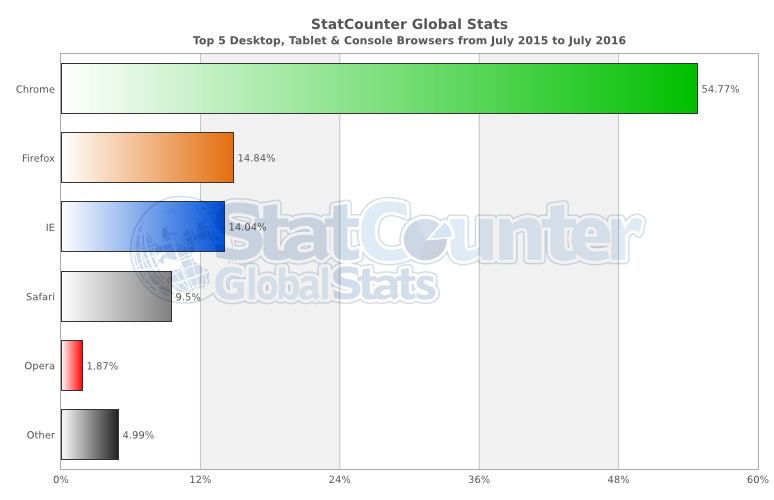
\includegraphics[scale=0.5]{obrazky/browsers}
\par\end{centering}
\caption{Zastoupení jednotlivých webových prohlížečů – červen 2016 \cite{statcounter} \label{fig:browsers}}
\end{figure}
\FloatBarrier
Syntaxe jazyka Javascript, pocházející z rodiny jazyků C++ a Java, je velkou výhodou pro vývojáře, kteří s ním začínají. Základním konstruktem Javascriptu je objekt, který reprezentuje všechny neprimitivní typy. Nezbytnou součástí jazyka je \textit{funkce}. Funkce je také instance typu Object a je možné s ní manipulovat jako s jakýmkoliv jiným objektem. Javascript implementuje takzvané \uv{first-class citizen funkce (prvotřídní funkce)}. To znamená že funkci lze uložit do proměnné a pracovat s ní jako s jakýmikoliv jinými daty \cite{flanagan_javascript}. Prvotřídní funkce je základním předpokladem pro funkcionální programování, které je pro javascript typické. Jeho funkcionální podstata dovoluje velice snadno vytvářet asynchronní anonymní funkce, které jsou pak registrovány jako obslužné funkce pro události. Událostí může být kliknutí uživatele na tlačítko, změna obsahu formulářového prvku, nebo načtení nové stránky. Pomocí protypové dědičnosti a takzvaných konstrukčních funkcí je také možné programovat do značné míry objektově. Javascript je implementovaný ve všech hlavních desktopových i mobilních webových prohlížečích a pomocí node.js jej lze provozovat i na serveru \cite{flanagan_javascript} \cite{hronek_javascript}. Jak lze vidět na následujícím grafu, Javascript je v současné době čtvrtým nejpoužívanejším jazykem \cite{skriptovaci_jazyky}. Také na serveru Github, který sdružuje git repozitáře zdrojového kódu má aktuálně (2016) Javascript nejvíce aktivních repozitářů, což vedle oblíbenosti tohoto jazyka, značí také ochotu javascriptových vývojářů uvolnit svůj kód jako open source \cite{githut}.
\vspace{0,3cm}
\begin{figure}[h]
\begin{centering}
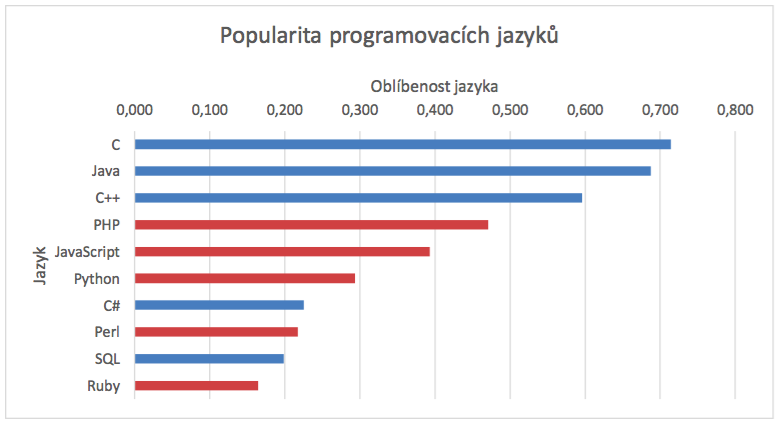
\includegraphics[scale=0.5]{obrazky/popularita_jazyku}
\par\end{centering}
\caption{Grap popularity programovacích jazyků, červeně označené skriptovací jazyky \cite{skriptovaci_jazyky} \label{fig:language-preferences}}
\end{figure}

\section{Historický vývoj}
Původní koncepce webových stránek nepočítala s použitím žádného programovacího jazyka, znala pouze HTML jako značkovací a CSS jako stylovací jazyk. Až v roce 1995 Brendan Eich představuje jazyk LiveScript, když pro společnost Netscape vymýšlí skriptovací jazyk, který chce firma využívat ve svém webovém prohlížeči. Firma krátce před jeho vydáním rozhodně o změně názvu na JavaScript\footnote{Dnes je rozšířenější označení Javascript, s malým \uv{s}, které budu používat i v této práci.}, kvůli tehdejší popularitě jazyka Java. Brzy po vydání první verze prohlížeče Netscape Navigator, přichází také společnost Microsoft se svým prohlížečem Internet Explorer. Ten také ve své verzi 3, vydané v roce 1996, podporoval Javascript, ačkoli byl jeho interpret kvůli obavám z licenčních sporů pojmenován jako JScript. Objevily se také některé další prohlížeče, které také dokázaly zpracovávat Javascript. V jednom okamžiku tedy existovalo několik rozdílných intepretů Javascriptu, což vynutilo potřebu standardizace tohoto jazyka. Byla založena organizace ECMA a vydán nový standard ECMA–262, který definoval skriptovací jazyk ECMAScript. Ten se stal základem pro různé implementace Javascriptu používané v různých webových prohlížečích. Javascript, který známe dnes, je také pouze jednou z implementací standardu ECMAScript. Díky jeho obrovské popularitě se ovšem tyto dva termíny často libovolně zaměňují. Existují však ještě další implementace jako JScript či ActionScript \cite{zakas_js} \cite{flanagan_javascript} \cite{hronek_javascript} .

Jednotlivé verze standardu ECMA se nazývají \textit{edice}, ta stále aktuální vyšla v červnu 2001 a nese označení 5.1 (dnes často nazývána ES5), v dnešních dnech (2016) je téměř dokončen přechod na verzi ES6, vydanou v roce 2015. Také byly záhájeny práce na vývoji další verze s pořadovým číslem sedm, která je očekávána v roce 2017. Některé nové vlastnosti ES7 jsou už implementovány v posledních verzích prohlížečů Mozilla Firefox a Google Chrome. Javascript se stal použitelnějším jazykem díky vývoji výkonných javacriptových běhových prostředí zejména ze strany společností Google a Mozilla \cite{hronek_javascript} \cite{ecmascript}. 
Na obrázku níže můžeme vidět běžné typy architektur webových aplikací, spolu s jejich výhodami a nevýhodami.
\begin{figure}[h]
\begin{centering}
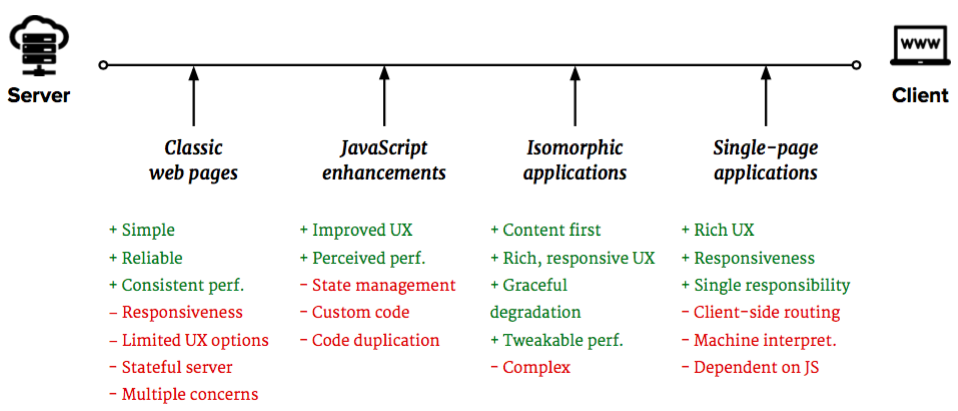
\includegraphics[scale=0.4]{obrazky/websites}
\par\end{centering}
\caption{Diagram typických architektur webových aplikací \cite{codepicnic_universaljs} \label{fig:typical-web-arch-diagram}}
\end{figure}
\FloatBarrier

\section{ES6 – Nové standardy}
Standard ES6, který definoval moderní podobu jazyka Javascript vyšel v srpnu 2015. Implementace standardů je však zdlouhavý proces, takže i když je standard ES6 téměř rok vydaný, kompletní podpora stále není implementována ve všech prohlížečích. Největší problém je tradičně u Internet Exploreru, kde i ten nejnovější jedenáctý ES6 téměř vůbec nepodporuje. V jiných prohlížečích se ES6 už těší velmi slušné podpoře. Potíž je však v tom, že ne všichni uživatelé používají poslední verze prohlížečů. V praxi je tak potřeba se ES6 zatím úplně vyhnout, nebo použít nějaký javascriptový transpiler (viz. \hyperref[sec:js_transpilers]{2.3}). Lepší situace je u node.js, kde poslední šestá verze má už 93\% podporu ES6 (viz. \hyperref[sec:node_js]{2.4}). Změnil se také proces, podle něhož se budou dostávat nové věci do prohlížečů. Vývoj standardu ES6 trval dlouhých 6 let, proto bylo nutné také navrhnout postup dalšího vývoje \cite{exploring_es6}. Nyní bude vznikat každý rok nová verze standardu ECMAScript \cite{tc39ecma}. Následuje přehled nejzajímavějších novinek nového standardu jazyka Javascript \cite{exploring_es6}.

\subsection{Třídy}
S nutností alespoň částečně používat Javascript téměř u každé webové aplikace, začalo tento jazyk používat stále více typických objektově orientovaných programátorů. Ti se snažily používat principy objektového návrhu i v Javascriptu. Základním kamenem objektového přístupu je \textit{třída}, kterou ale Javascript vůbec nezná. Také nezná klasickou dědičnost, místo toho obsahuje takzvanou protypovou dědičnost. Ta zjednoduše řečeno umožňuje definovat prototyp, ze kterého bude každý objekt daného typu vytvořen. Až standard ES6 přináší nové klíčové slovo \textit{class}, které usnadňuje objektově orientované programování v jazyce Javascript. Je již tedy možné definovat třídu, její kontruktor, provádět volání rodičovské metody nebo implementovat statické metody. Je také možné dědit jinou třídu pomocí klíčového slova \textit{extends}, které realizuje již zmíňenou prototypovou dědičnost na pozadí. Mnoho zkušenejších javascriptových vývojářů ale zastává názor, že přidání této syntaxe je velká chyba. Bude totiž svádět vývojáře ke klasickému OOP, což je v Javascriptu z mnoha důvodů považováno za špatné \cite{exploring_es6} \cite{es6} \cite{es6_book}.
\begin{lstlisting}[language=Javascript,caption={Ukázka ES6 syntaxe pro třídy v Javascriptu \cite{es6}}]
class SkinnedMesh extends THREE.Mesh { // definice třídy
  constructor(geometry, materials) { // konstruktor
    super(geometry, materials);

    this.idMatrix = SkinnedMesh.defaultMatrix();
    this.bones = [];
    this.boneMatrices = [];
    //...
  }
  update(camera) { // třídní metoda
    //...
    super.update();
  }
  static defaultMatrix() { // statická metoda
    return new THREE.Matrix4();
  }
}
\end{lstlisting}

\subsection{Let a const}
\label{sec:variable_scope}
Jednou z nejkritizovanějších vlastností jazyka Javascript je globální kontext všech funkcí a proměnných. Definování proměnné na jakémkoliv místě znamená její uložení do globálního kontextu aplikace. Opětovné definování proměnné pod stejným názvem neskončí chybou, ale přepsáním původní hodnoty. To může přinášet nečekané problémy například nováčkům. Ovšem jako u každé nevýhody Javascriptu, našla komunita několik běžně používaných řešení. Nejčastěji se jedná o obalení kódu javascriptovou anonymní funkcí, které je vykonána ihned po deklaraci. Jedná se o takzvanou IIFE (Immediately-Invoked Function Expression) \cite{exploring_es6} \cite{es6} \cite{es6_book}.

\begin{lstlisting}[language=Javascript,caption={IIFE – řešení lokálního kontextu v ES5 Javascriptu. \cite{exploring_es6}}]
(function () {  // začátek IIFE
    var tmp = "something";
}());  // ukončení a zavolání IIFE

console.log(tmp); // ReferenceError, tmp není na globálním kontextu definováno
\end{lstlisting}

ES6 ovšem problém globálního kontextu řeší zavedením nových klíčových slov \textit{let} a \textit{const}. Příkaz let oproti běžnému var omezuje kontext proměnné na nejbližší blok. Const definuje neměnitelnou konstantu \cite{exploring_es6} \cite{es6} \cite{es6_book}.
\begin{lstlisting}[language=Javascript,caption={Ukázka nových klíčových slov pro proměnné v ES6 Javascriptu \cite{exploring_es6}.}]
function fn() {
  {
    let x;
    {
      // platnost pouze v tomto bloku
      const x = "sneaky";
      // chyba, nemůžeme měnit konstantu
      x = "foo";
    }
    // chyba, nemůžeme opět deklarovat x ve stejném bloku
    let x = "inner";
  }
  console.log(x); //ReferenceError není definováno na tomto bloku
}
\end{lstlisting}
\subsection{Moduly}
Nezbytnou vlastností každého moderního programovacího jazyka je podpora modularizace, původní Javascript podle očekávání žádnou vestavěnou podporu nemá. Nezná ani klíčové slovo \textit{include}. Bylo tedy nutné přinést nějaké řešení, dnes existuje několik konvencí pro javascriptové moduly jako Common.js, AMD nebo UMD. Ty popisují API, která zaručují správnost jeho načtení a následné komunikace. Samotná modularizace je také často v Javascriptu realizována pomocí vlastních kličových slov (například \textit{require()}), postprocesor potom spojí jednotlivé moduly v jeden velký javascriptový soubor, ze kterého je potom celá aplikace spuštěna. Nejznámější z nich je \textit{browserify} nebo také čím dál oblíbenejší \textit{webpack}. Postprocessor prochází soubory webové aplikace počínaje výchozím bodem (entrypointem) aplikace a hledá v nich deklarace závislostí na dalších souborech. Tento přístup zajišťuje použití jen skutečně využívaného kódu. V dřívejších dobách obsahoval každý postprocesor pro definici zdrojů vlastní syntaxi, dnes se téměř výhradně používá syntaxe dle ES6. Standard ES6 totiž přináší nové klíčové spolo \textit{import}, které dodává do Javascriptu tolik postrádanou možnost načítání externích zdrojů. Načítání může být konečně řešeno na straně jazyka a není nutné ho realizovat pomocí specializovaných nástrojů. Mechanismus sestavení jednoho výstupního souboru obsahujícího celou aplikaci však zůstal zachován, je nutný pro zmenšení datové náročnosti a počtu dotazů výsledné webové aplikace \cite{exploring_es6} \cite{es6} \cite{es6_book}. Následuje popis nových klíčových slov jazyka Javascript usnadňujících práci s moduly.

\vspace{3mm}
Ze souboru můžeme exportovat funkce, objekty i proměnné pomocí klíčového slova \textit{export} \cite{es6}.
\begin{lstlisting}[language=Javascript,caption={Deklarace modulu v ES6 Javascriptu \cite{es6}}]
// lib/math.js
export function sum(x, y) {
  return x + y;
}
export var pi = 3.141593;
\end{lstlisting}

V jiném souboru si je pak můžeme importovat pomocí klíčových slov \textit{import} a \textit{from}. Použijeme-li znak hvězdičky (*) naimportujeme z externího souboru vše. Můžeme si ale i vybrat, které části modulu potřebujeme pomocí \textit{destructuringu} (viz níže) \cite{exploring_es6} \cite{es6} \cite{es6_book}.
\begin{lstlisting}[language=Javascript,caption={Použití modulu v ES6 Javascriptu \cite{es6}}]
// app.js
import * as math from "lib/math"; //import všeho z lib/math.js
alert("2pi = " + math.sum(math.pi, math.pi)); // přibyl nový objekt math

import {sum, pi} from "lib/math"; //import jen některých částí z lib/math.js
alert("2pi = " + sum(pi, pi)); // na lokálním kontextu přibyly nové objekty sum a pi
\end{lstlisting}
Specialitou je nové klíčové slovo \textit{default}. To definuje, která část souboru se importuje, není li explicitně řečeno která část se má použít. V cílovém souboru si můžeme default import pojmenovat zcela dle své vůle (zde exp). Současně můžeme i nadále importovat ostatní funkce, objekty a proměnné \cite{exploring_es6} \cite{es6} \cite{es6_book}.
\begin{lstlisting}[language=Javascript,caption={Použití modulu s klíčovým slovem default v ES6 Javascriptu \cite{es6}}]
// lib/mathplusplus.js
export * from "lib/math";
export var e = 2.71828182846;
export default function(x) {
    return Math.exp(x);
}

// použití
// app.js
import exp, {pi, e} from "lib/mathplusplus";
alert("2pi = " + exp(pi, e));
\end{lstlisting}

\subsection{Další novinky}
Standard ES6 přinesl také mnoho dalších novinek, velmi užitečné jsou výchozí hodnoty argumentů funkcí, šablony pro řetězce nebo destructuring. Dále naleznete ukázky použití posledních dvou zmíněných novinek: šablon pro řetězce, které se uvozují takzvaným \textit{backtick operátorem} ( {\large \textbf{`}} ) a \textit{destructuringu}. Ten umožňuje využít jen některé exportované části importovaného modulu. Často se používá pro získání jen některých funkcí nějaké externí knihovny, například hypotetický zápis \textit{const \{ajax,cookies\} = angular} by získal z frameworku AngularJS jenom moduly zodpovědné za podporu AJAX operací a správu cookies \cite{exploring_es6} \cite{es6} \cite{es6_book}.

\begin{lstlisting}[language=Javascript,caption={Ukázka použití šablon pro řetězce v ES6 \cite{exploring_es6}. }]
//ES5 syntaxe
function printCoord(x, y) {
    console.log('(X='+x+',Y= '+y+')');
}
//ES6 syntaxe
function printCoord(x, y) {
    console.log(`(X=${x}, Y=${y})`);
}

\end{lstlisting}

\begin{lstlisting}[language=Javascript, caption={Ukázka použítí destructuringu v ES6 \cite{exploring_es6}}]
const obj = { first: 'Jane', last: 'Doe' };
const {first, last} = obj;
    // first = 'Jane'; last = 'Doe'
\end{lstlisting}

\section{Javascriptové transpilery}
\label{sec:js_transpilers}
Standard ES6 přináší dva základní typy novinek.  První jsou nová rozhraní nebo rozšíření těch existujících, tyto změny můžeme ve starším Javascriptu simulovat pomocí mnoha knihoven, které se nazývají shimy nebo polyfilly. Ty dokážou detekovat podporu moderního Javascriptu a případné chybějící funkce doplnit. V budoucnu, až bude většina používaných webových prohlížečů plně podporovat ES6, mohou být tyto knihovny odstraněny. Druhou novinkou je nová syntaxe, například nová klíčová slova \textit{class}, \textit{extends}, \textit{let} či \textit{import}. Změny v samotné syntaxi Javascriptu již nejde simulovat nějakou knihovnou, je nutné používat program – kompilátor, který náš kód přeloží do aktuálně plně podporované verze Javascriptu, tedy do ES5. Protože se jedná o převod mezi programovacími jazyky stejné úrovně, používá se označení \textit{transpiler} nebo \textit{source-to-source kompilátor}. Zpětný překlad není většinou možný. Javascriptový transpiler, mimo převodu kódu na starší verzi, provede také doplnění všech nutných polyfillů, aby byla zajištěna funkčnost na většině současných prohlížečů \cite{learning_es6} \cite{transpilers}.

Jedná se o stejný přístup jako u kompilátorů skriptovacích jazyků, které jsou do Javascriptu překládány. Z nejznámějších lze zmínit CoffeeScript nebo Purescript. Tyto jazyky vznikly před příchodem ES6, aby syntakticky zjednodušily vývoj v Javascriptu. Dnes je doporučované používat ES6 a oblíbenost těchto jazyků začíná klesat. Javascriptové transpilery lze tedy rozdělit do dvou základních kategorií. První jsou zcela nové jazyky, které mají úplně odlišnou syntaxi a nemůžeme je tedy použít na vylepšení již hotových projektů. Druhou představují jazyky, které Javascript jen rozšiřují a snaží se zachovat maximální dopřednou kompatibilitu. Mezi takové řadíme i BabelJS \cite{babel}, který je popsán níže \cite{learning_es6} \cite{transpilers}.

\begin{enumerate}
\item \textbf{používající vlastní vstupní jazyk} – CoffeeScript, PureScript, Script\#, Haxe
\item \textbf{kompilující moderní Javascript do současného} – Babel, TypeScript, Traceur 
\end{enumerate}

\subsection{CoffeeScript}
CoffeeScript je nový programovací jazyk, který se kompiluje do Javascriptu. Byl vytvořen pro zjednodušení syntaxe původního Javascriptu, odstraňuje z něj středníky, závorky a také zavádí definici tříd typickou pro objektově orientované jazyky. Při svém vývoji byl inspirován syntaxí jazyka Ruby, ve kterém byl napsán i první překladač, současné verze překladače je již napsána v Javascriptu, respektive samotném CoffeeScriptu. První verze byla vydána v roce 2009 a jeho autor Jeremy Ashkenas do první commit message napsal: \uv{initial commit of the mystery language}, což lze přeložit jako první commit záhadného jazyka \cite{coffeescript_founder}. První stabilní verze vyšla na Vánoce roku 2010. CoffeeScript se běhěm několika let stal velmi populárním. Někteří vývojáři však zastávají názor, že zjednodušení syntaxe naopak zhoršilo čitelnost výsledného kódu. Velkou nevýhodou je špatné odhalování programátorských chyb, protože chyba se zobrazí ve vygenerováném javascriptovém kódu. Až po jejím pochopení je možné ji dekódovat na úrovni CoffeeScriptu. Na druhou stranu ke každému kódu v CoffeeScriptu existuje ekvivaletní kód v Javascriptu, a proto lze při vývoji používat jakékoliv javascriptové knihovny \cite{coffeescript}.

\begin{table}[h]
\centering
	\caption{Ukázka syntaxe CoffeeScriptu spolu s překladem do Javascriptu \cite{coffeescript} \label{fig:js_vs_coffee}}
	\begin{tabular}{ |p{5cm}|p{5cm}| }
	\hline
	CoffeeScript & Javascript \\ \hline
	number = -42 if opposite & 
	\begin{minipage}[t]{0.2\columnwidth}%
       if(opposite)\{
          \newline
          number = -42;
          \newline
          \}
    \end{minipage}	
	\\ \hline
	squere = (x) -> x * x &	
	\begin{minipage}[t]{0.2\columnwidth}%
       var square = function(x) \{
          \newline
          return x * x;
          \newline
          \};
    \end{minipage}
    \\ \hline
    alert "I knew it!" if elvis? &
    \begin{minipage}[t]{0.4\columnwidth}%
       if(typeof elvis !=="undefined" 
          \newline
          \&\& elvis !==null)\{
          \newline
          alert("I knew it!");
          \newline
          \}
    \end{minipage}
    \\ \hline
	\end{tabular}
	\label{tab:coffeescript}
\end{table}

\subsection{Babel}
\label{sec:babel}
Aby bylo možné používat Javascript ES6 už dnes a nečekat několik let než se dostane alespoň do posledních verzí prohlížečů, vznikl projekt Babel. Ten představuje transpiler ES6 kódu do verze ES5, kterou umí většina současných prohlížečů. Babel vznikl v roce 2015 jako projekt 6to5 a rychle si získal velkou oblíbenost mezi javascriptovými vývojáři a jeho využití stále stoupá. Hlavním důvodem je nejširší podpora standardu ES6 včetně některých nových vlastností ES7. Babel také plně integruje JSX a je tedy více než vhodný pro použití s frameworkem React. Příchod Babelu bude také nejspíš znamenat snižování ochoty vývojářů používat jiné jazyky, které se kompilují do Javascriptu, protože bude jistější používat něco, co je standardizované než vlastní jazyk vymyšlený nějakou společností nebo vývojářem. Babel lze také používat v node.js, i když tempo zavádění ES6 do node.js je výrazně rychlejší než u webových prohlížečů. Kvůli různým javascriptových prostředím, kde cílový kód poběží, obsahuje Babel takzvané \uv{presety}. Pomocí nichž lze nastavit na jakou verzi Javascriptu má provést překlad kódu, které lze rozdělit na dvě základní skupiny. Prvním skupinou jsou webové prohlížeče. Zde záleží především na potřebě kompatibility aplikace s prohlížečem Internet Explorer. Druhou skupinou je node.js, kde každý preset odráží novou verzi tohoto frameworku. V budoucnu až node.js tým dokončí plnou implementaci standardu ES6, nebude využití Babelu v node.js nutné. Výběr vhodného presetu je na vývojáři, který musí zvážit jaké prohlížeče ještě chce podporovat a jaké už ne. Knihovna Babel ve výchozím stavu kompiluje Javascript kompletně do ES5, výsledek by měl být funkční ve většině současných prohlížečů počínaje Internet Explorerem 9 \cite{babel} \cite{babel_what}. Následuje ukázka konverze nového zápisu pro funkce z ES6.
\vspace{0,3cm}
\begin{figure}[h]
\begin{centering}
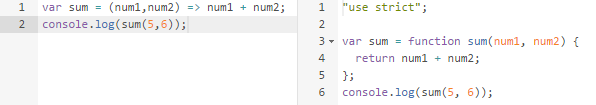
\includegraphics[scale=0.6]{obrazky/babel}
\par\end{centering}
\caption{Ukázka konverze ES6 javacriptu do ES5 pomocí transpileru Babel \cite{babel} \label{fig:babel}}
\end{figure}
\FloatBarrier

Babel dnes používají největší internové společnosti jako Facebook, Yahoo, Netflix, Mozilla nebo Evernote \cite{babel}.

\section{Node.js – Javascript na serveru}
\label{sec:node_js}
Důležitým pokrokem ve světě Javascriptu bylo představení platformy Node.js, která umožnila spouštění javascriptového kódu na serveru. S nárůstem oblíbenosti tohoto jazyka jistého člověka napadlo vzít javascriptové jádro V8 z prohlížeče Google Chrome a postavit nad ním velmi výkonnou platformu, použitelnou i mimo webový prohlížeč, zejména na serverech. Tím člověkem byl Ryan Dahl a celá platforma, která byla navržena s ohledem na dobrou škálovatelnost vycházející z principu asynchronního zpracování kódu v jednom vlákně, byla v roce 2009 uvolněna jako open source. Engine V8, napsaný v C++, kompiluje Javascriptový kód do nativního a nejen díky tomu je jedním z nejvýkonnějších javascriptových enginů. Tím pádem bylo jeho použití ideální. Jeho nápad se setkal s obrovským ohlasem a dnes node.js tvoří nepostradatelnou část javascriptového ekosystému. Node.js je zaměřené na dlouhodobě běžící serverové procesy, na rozdíl od jiných prostředí ale neumí využívat více vláken najednou (multithreading). Místo toho využívá čistě asynchronní povahu jazyka Javascript a veškeré operace provádí v jednom hlavním vlákně. Server se tedy chová jako démon\footnote{Termínem démon se v IT prostředí označuje specifický program, který svou činnost provozuje dlouhodobě a vůbec nemusí být nijak závislý na přímém kontaktu s koncovým uživatelem (jejich vzájemné interakci).} spouštějící javascriptový interpret. V poslední době se však objevují snahy vícevláknové operace do node.js doplnit \cite{nodejs} \cite{glover_nodejs} \cite{tilkov_nodejs}.

\begin{lstlisting}[language=Javascript,caption=Ukázka kompletní implementace programu Hello World v node.js]
var http = require('http');
http.createServer(function (request, response) {
    response.writeHead(200, {'Content-Type': 'text/plain'});
    response.end('Hello World\n');
}).listen(8000);

console.log('Server running at http://localhost:8000/');
\end{lstlisting}

Výše uvedený příklad kódu je kompletní implementací webového serveru, zobrazujícího text \textit{Hello World} v node.js. Na prvním řádku můžeme vidět získání závislosti na webovém serveru, pro které má node.js speciální funkci \textit{require}. Funkcionální přístup javascriptu je pro úlohy jako webové server ideální, ukázkový kód je proto velmi krátký. V lednu 2010 byl také přestaven balíčkovací systém \textit{npm}, který řeší správu, instalaci a aktualizaci javascriptových balíčků. Z počátku byl používán jen pro node.js, v současnosti již proniká i do vývoje frontendových částí aplikací, tedy do webových prohlížečů. Dnes má npm více než 250 000 stažených balíčků každý den \cite{nodejs_numbers}. Každá aplikace využívající pro zprávu závislostí npm obsahuje v hlavním adresáři soubor \textit{package.json}, který definuje celou npm aplikaci. Tento soubor obsahuje popisná data o aplikaci, závislosti na externích knihovnách včetně verzí (je možné definovat také závislosti určené jen pro vývoj), umístění repozitáře, vstupní bod aplikace nebo například typ licence. Npm je kompletně ovládáno z příkazové řádky. Pomocí příkazu \textit{npm install} dojde \uv{nainstalování}  aplikace, jsou tedy staženy a nainstalovány veškeré závislosti a aplikace připravena ke spuštění. Npm také nově umožňuje definici úkolů pro vestavěný task runner (viz \hyperref[sec:task_runner]{2.6}), kterým lze webovou aplikaci dále spravovat \cite{glover_nodejs} \cite{tilkov_nodejs} \cite{npm}.

\begin{lstlisting}[language=Javascript, caption=Soubor package.json definující závislosti pro NPM]
{
  "name": "amazing-js-app",
  "version": "0.2.0",
  "description": "A amazing js app written in Javascript",
  "main": "index.js", //vstupní bod aplikace
  "scripts": {
    "start": "node index.js" // úkoly pro task runner
  },
  "dependencies": { // zavislosti
    "express": "^4.13.3"
    ...
  },
  "devDependencies": { //zavislosti pro vývoj
    "mocha": "^4.13.3"
    ...
  },
  "repository": { //umístění repozitáře
    "type": "git",
    "url": "https://github.com/jakub.josef/amazing-js-app"
  },
  "keywords": [
    "amazing",  "js",  "app"
  ],
  "author": "Jakub Josef",
  "license": "MIT"
}
\end{lstlisting}

I když není ještě zastoupení javascriptových serverů příliš vysoké, tento trend již několik let roste. Dle Tilkov, Vinosky pro to existuje několik hlavních důvodů. Jedním z nich je nástup technlogií pod značkou HTML5, které vytlačují alternativní platformy na straně klienta, jako například Adobe Flash nebo Microsoft Silverlight, kde je nutné použít Javascript. Je pak více než vhodné použít stejný jazyk i na serveru \cite{tilkov_nodejs}.

Zajímavou knihovnou je také Electron, přes který lze psát pomocí node.js klasické desktopové aplikace a je v něm napsaný třeba textový editor Atom.io nebo klient pro komunikátor Slack \cite{elektron}. 

\section{Vývojové nástroje}
S nárůstem oblíbeností Javascriptu vzniklo obrovské množství knihoven\footnote{Občas se objevují pokusy rozlišit termíny knihovna a framework, v této práci budou používány víceméně ekvivalentně.} a nástrojů, které usnadňují proces vývoje. Typické vývojové prostředí se skládá s desítek knihoven usnadňující práci se šablonami, získávání dat nebo testování. Je tedy nutné používat nějaký skript nebo program, který bude celé vývojové prostředí řídit. Ve světě Javascriptu se příliš neuchytilo používání velkých IDE\footnote{Integrated Development Environment – kompletní vývojářské prostředí, například Eclipse, Intellij IDEA nebo Netbeans IDE}. Místo toho se využívá takzvaných \textit{task runnerů}, kteří mají definovány relevantní úkoly, například sestavit aplikaci a spustit vývojový webový server, aktivovat testy, nebo vytvořit balíček pro produkční nasazení. Task runner se zpravidla ovládá pomocí příkazové řádky. Typické vývojové prostředí je pro moderní aplikace v Javascriptu velmi komplexní a jeho prvotní konfigurace může být složitá. Je to proto, že na takové prostředí jsou dnes kladeny vysoké požadavky. Jsou to například: \cite{flanagan_javascript} \cite{task_runners} 

\vspace{0.5cm}
\begin{itemize}
\item programování v ES6 Javascriptu, možnost použití transpileru,
\item škálovatelnost výsledné aplikace,
\item maximální modularita,
\item možnost jednoduše integrovat a používat stovky tisíce balíčků z npm,
\item používat nějaký CSS preprocesor, 
\item po každé změně v kódu by měl být ihned vidět výsledek v prohlížeči (livereload),
\item vývojový a produkční mód,
\item v produkčním módu všechny potřebné JS soubory (moduly) sloučit do jednoho a minimalizovat, obdobně i pro kaskádové styly,
\item v produkčním módu ignorovat warningy a jiné debugovací výpisy,
\item kontrola (lintování) kódu,
\item spouštění testů uvnitř webového prohlížeče.
\end{itemize}

\section{Automatizace vývoje}
\label{sec:task_runner}
Jak je již zmíněno, vývojové prostředí většinou obsahuje větší množství knihoven a nástrojů, jejichž vzájemnou interakci řeší task runner. Ten umožňuje definovat úkoly (tasky), které provedou nějakou činnost. Typicky se jedná například o minifikaci JS kódu nebo obsluhu vývojového webového serveru. Tomuto přístupu se říká \textit{automatizace vývoje} a je ve světě moderního Javascriptu naprosto zásadní. Prvním populárním programem tohoto typu byl \textit{Grunt} \cite{grunt}, dnes je mezi vývojáři oblíbenější jeho přímý konkurent Gulp, který je použit i v této práci. Gulp vyniká především jednodušší konfigurací a větším výkonem \cite{gulp}. Většinu takových úkolů pro běžně používané knihovny není nutné programovat, lze je nalézt v balíčkovacím systému NPM, a to pro oba zmíněné automatizační nástroje. Úkoly je do sebe možné libovolně zanořovat a volat je v určeném pořadí.  Je také možné použít připravené vývojové prostředí, takzvaný \uv{devstack}. Ten obsahuje mnoho hotových úkolů, usnadňujících vývoj. Jejich použítí je dnes doporučované, existují desítky devstacků pro všechny nejpoužívanější javascriptové webové frameworky \cite{task_runners}. Představení několika z nich naleznete v kapitole \hyperref[sec:devstacks]{4.6}.

\vspace{3mm}
\noindent Task runner Gulp ukládá konfigurace do souboru Gulpfile.js \cite{gulp} \cite{gulp_web}. Následující ukázka kódu demonstruje jednoduchost jeho konfigurace.

\begin{lstlisting}[language=Javascript,caption={Ukázka konfigurace task runneru Gulp \cite{gulp}}]
// načtení externích knihoven
var gulp = require('gulp')
, fs = require('fs')
, coffeelint = require("gulp-coffeelint")
, coffee = require("gulp-coffee")
, uglify = require("gulp-uglify")
, concat = require("gulp-concat")
, header = require("gulp-header");
 
// definice úkolu bundle
gulp.task('bundle', function () {
    gulp.src('./coffee/*.coffee') // cesta ke zdrojovým souborům
    .pipe(coffeelint()) // lintování
    .pipe(concat('bundle.js')) // spojení souborů do jednoho s názvem bundle.js
    .pipe(coffee()) // kompilace CoffeeScriptu
    .pipe(uglify()) // minifikace zkompilovaného Javascriptu
    .pipe(gulp.dest('./dist')); // uložení do adresáře dist
});
\end{lstlisting}

Task runner Gulp je hluboce založen na takzvaných streamech (česky datových proudech), každý stream provádí vždy určitou činnost, na vstup přijímá cestu k souboru nebo jiný stream a jeho výsledky mohou být zapsány do souboru nebo předány dalšímu streamu \cite{gulp_web}. Výše uvedená konfigurace definuje úkol (task) \textit{bundle}, který provede následující v daném pořadí:
\begin{enumerate}
\item načtení CoffeeScript kódu z adresáře coffee
\item kontrola (lintování) CofeeScript kódu
\item spojení všech souborů v jeden
\item kompilace CoffeeScriptu
\item minifikace (odstranění mezer a zkrácení kódu) vygenerováno Javascriptu
\item uložení výsledku do adresáře dist
\end{enumerate}

\section{Lintování kódu}
Takzvané \uv{lintování} kódu je proces, který pomáhá sjednotit vzhled a zajistit formální správnost zdrojového kódu celé aplikace. Program, který tyto kontroly provádí se nazývá linter. Ten hlídá styl kódu, korektní používání závorek či odsazení. Pravidla, kterými se řídí jsou dány aktuálními standardy v lintovaném jazyce, ty je možné upravit, nebo si definovat vlastní. Linter také umí odhalit některé překlepy nebo nepoužívané konstrukce. Pro jazyk Javascript se dlouhou dobu používal nástroj JSHint, který dnes nahrazuje ESLint, který přináší především podporu modularity. Je tedy možné jej rozšířit o validování Babel syntaxe nebo JSX komponent z frameworku React. Lintování kódu bývá zpravidla součástí build procesu, aby se odhalily nedostatky před vytvořením nové verze aplikace \cite{flanagan_javascript} \cite{linter}.

\begin{figure}[h]
\begin{centering}
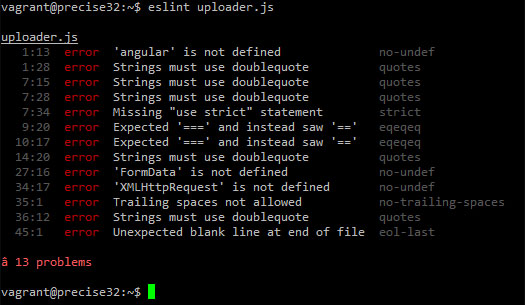
\includegraphics[scale=0.6]{obrazky/linter}
\par\end{centering}
\caption{Ukázka výstupu linteru ESLint \cite{linter} \label{fig:linter}}
\end{figure}
\FloatBarrier

\section{Nejpoužívanejší knihovny}
Naprosto zásadní věcí při výběru programovacího jazyka je existence kvalitních a dobře dokumentovaných knihoven. Jazyk Javascript jich obsahuje obrovské množství a výběr mezi nimy není jednoduchý. Existuje několik zásadních knihoven, které do značné míry ovlivnily vývoj tohoto jazyka. Následující kapitola obsahuje popis tří z nich, dle mého názoru pro svět Javascriptu nejzásadnějších. Všechny zmíněné knihovny jsou open source a je možné je používat zdarma.

\subsection{jQuery}
Pravděpodobně první knihovnou, která se běžnému webovému vývojáři vybaví ve spojení s jazykem Javascript je jQuery. Poprvé ji představil John Resig v roce 2006. Knihovna jQuery odstartovala masivní využívají Javascriptu ve webových aplikacích především zjednodušením někdy složité javascriptové syntaxe a velmi dobře zpracovanou dokumentací s příklady \cite{jquery} \cite{jquery_book}. 

\vspace{3mm}
\noindent Knihovna jQuery obecně přináší především tyto funkce \cite{jquery}.
\begin{itemize}
\item \textbf{Podpora všech moderních prohlížečů} – jQuery odstraní většinu problému s kompatibilitou poskytnutím unifikovaných rozhraní, které jsou schopné přizpůsobení používanému prohlížeči.
\item \textbf{Práce s DOM} – jQuery umožňuje snadno vyhledávat a měnit DOM elementy. Vyhledávání DOM elementů, které probíhá pomocí CSS selektorů, se stalo tak populární, že patřičnou funkci pro vyhledávání pomocí CSS selektorů dnes obsahuje i čistý Javascript.
\item \textbf{Rozhraní pro AJAX} – Moderní webové aplikace jsou kompletně postaveny na asynchronních HTTP voláních. Framework jQuery usnadňuje jejich obsluhu a zpracování serverové odpovědi.
\end{itemize}

jQuery také zavedlo znak dolaru (\$) pro funkci DOM selektoru, který se používá pro získávání HTML entit javascriptem. Například selektor \emph{\$("div.some-class");} získá všechny div elementy, které mají třídu \textit{some-class}. Tuto konvenci pro získávání DOM elementů převzaly i některé jiné frameworky a dnes je de facto standardem. Na takto získaném HTML elementu lze provádět mnoho operací, nejčastější z nich jsou popsány v tabulce \hyperref[tab:jquery]{2.2}. Mnoho z těchto funkcí je duálního charakteru, při jejich zavolání bez parametru se chová jako getter, s parametry jako setter \cite{jquery_book}.
\begin{table}[h]
\centering 
	\caption{Přehled nejpoužívanějších funkcí frameworku jQuery pro manipulaci s DOM elementy\label{tab:jquery}}
		\begin{tabular}{ |p{3cm}|p{7cm}| }
	\hline
	Název funkce & Popis funkce \\ \hline
	find() & vyhledávání DOM elementů uvnitř aktuálního elementu \\ \hline
hide() & skrytí elementu \\ \hline
show() & zobrazení elementu \\ \hline
html() & nastavení HTML obsahu elementu nebo jeho získání (bez parametru)\\ \hline
append() & přidání jiného elementu \textbf{za} aktuální element\\ \hline
prepend() & přidání jiného elementu \textbf{před} aktuální element \\ \hline
on() & navěšení listener funkce\footnote{Funkce, která bude zavolána dojde li kd dané události, například kliku na tlačítko \label{note:listener}} \\ \hline
off() & odebrání listener funkce\footnotemark[\value{footnote}] \\ \hline
css(): & nastavení CSS stylu nebo jeho získání (v závislosti na počtu parametrů) \\ \hline
attr() & získání nebo nastavení HTML atributu (např. disabled) \\ \hline
val(): & získání nebo nastavení hodnoty atributu (pro formulářové prvky) \\ \hline
text() & vrátí textové HTML elementu\\ \hline
each() & provede předanou funkci na všech získaných elementech \\ \hline
	\end{tabular}
	\label{tab:coffeescript}
\end{table}
\FloatBarrier

\pagebreak
Využití knihovny jQuery výrazně usnadňuje práci webového vývojáře oproti použití čistého Javascriptu, jehož konstrukce jsou v některých případech zbytečně složité. Výsledkem je obvykle kratší a pochopitelnější kód než v čistém Javascriptu. jQuery se díky tomu stalo nejznámějším javascriptovým frameworkem, které dnes nalezneme téměř na každém webu, ať klasického, tak jednostránkového charakteru \cite{jquery_book}. 
Existuje také projekt jQuery UI, který poskytuje sadu hotových javscriptových widgetů pro tvorbu webových aplikací. Jedná se například o kalendář, datepicker (formulářový prvek pro výběr datumu), modální okno, slideshow a další \cite{jquery_ui}.
\subsection{AngularJS}
Dalším zástupcem nejznámějších javascriptových frameworků je AngularJS. AngularJS slouží k naprosto jinému účelu než výše zmíněné jQuery.
Jedná se o MVC framework, jehož základní myšlenkou je použít deklarativní programování i pro tvorbu dynamických webových aplikací. Rozšiřuje za tímto účelem HTML o další značky. Původně byl vytvořen slovenským programátorem Miško Heverym, který projekt udržoval pod záštitou společnosti Google. Pro základní práci s DOM (Document Object Model) může spolupracovat s jinými knihovnami včetně jQuery. Jednou z hlavní předností AngularJS je obousměrný data binding. Ten zajišťuje automatickou synchronizaci modelu a pohledu. Celý princip dobře ilustruje obrázek \hyperref[fig:twoway-angular]{2.6}. V jiných frameworcích je třeba tuto činnost řešit ručně. Tato funkce, která do značné míry zapříčiníla vysokou oblíbenost a rychlou adaptaci tohoto frameworku, je však dnes kritizována pro svojí vysokou výpočetní náročnost a Angularu podobné frameworky jí nikdy neobsahovaly. Také nová verze AngularJS 2 pracuje s \uv{jednosměrným data-bindingem}, tedy pouze směrem z modelu do pohledu. Při každé změně modelu je tedy nutné překreslit celý pohled. Tato operace je sice celkem výpočetně náročná, neprobíhá ale tak často jako obslužná logika obousměrného data bindingu. Angular také používá techniku \textit{deep linkingu}. Deep-linking určuje pohled na webovou aplikaci, řeší kde se uživatel nachází a podle toho rozhoduje, jaké zobrazení bude vyvoláno. K tomuto účelu používá HTML kotvu (\#) doplněnou za aktuální URL \cite{angular} \cite{spa_horyna}.

\begin{figure}[h]
\begin{centering}
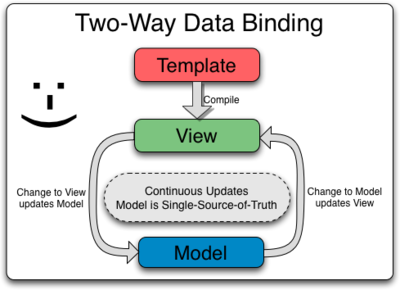
\includegraphics[scale=0.65]{obrazky/twoway_databinding}
\par\end{centering}
\caption{Diagram obousměrného data bindingu knihovny AngularJS \cite{angular} \label{fig:twoway-angular}}
\end{figure}
\FloatBarrier

AngularJS také řeší správu závislostí jednotlivých částí aplikace, a to podle principu \textit{Dependency Injection}, který odebírá třídám zodpovědnost za získání závislostí. Řešení je její převedení na standardizovaný kontajner, který závislosti třídám předává při jejich vytvoření. Framework také poskytuje rozhraní pro sledování změn v modelu (tzv. watchers) a celkově usnadňuje obsluhu událostí. Další z oblíbených vlastností je možnost definice vlastních znovupoužitelných HTML komponent zde nazvaných direktivy. Direktiva v AngularJS je fakticky vlastní HTML element, který zobrazovací logika frameworku převede na běžné HTML dle definice direktivy \cite{angular}.

\subsection{React}
\label{sec:react}
Po nějaké době používání velkých javascriptových MVC frameworků typu AngularJS, které řeší vše uvnitř webového prohlížeče, se začaly projevovat nevýhody toho přístupu. S rozmachem node.js přicházely názory, že je nutné část logiky přesunout zpět na server. Vývojáři moderních webových aplikací, kteří nechtěli používat klasické MVC frameworky, hledali framework vhodný pro jednoduší webové aplikace. Takový, který by řešil jen pohledovou vrstvu, která po přesunutí aplikační logiky na server zůstane webovému prohlížeči. Objevili React. React, což je knihovna pro vytváření uživatelského rozhraní, která řeší pouze pohledovou vrstvu aplikace, tedy jen pomyslné písmeno V z principu MVC. Samotný framework React vznikl jako opensource projekt již v květnu 2013 ve společnosti Facebook. V době vydání byl komunitou přijat převážně negativně, dokonce tak negativně, že společnost Facebook uvažovala o jeho stažení. K tomu ale nakonec nedošlo. React byl jako takový doceněn až v roce 2015, kdy začal být hojně používán pro programování isomorfních webových aplikací. Tedy takových, které používají jazyk Javascript i na serveru. V této době začínali vývojáři postupně opouštět velké monolitické MVC frameworky a přecházet k velmi modularním javascriptovým aplikacím, složených z mnoha knihoven. Dnes má React více než 6000 commitů a kolem 700 přispěvovatelů na serveru Github a je tak jedním z nejoblíběnějších a nejaktivnějších git repozitářů. Úspěch frameworku React také započal opensourcování dalších interních javascriptových projektů společnosti Facebook, jako například immutable.js nebo React Native (pro mobilní telefony). Dnes jsou nástroje společnosti Facebook jedněmi z nejpoužívajších při vývoji moderních webových aplikací v Javascriptu \cite{spa_horyna} \cite{react} \cite{react_book}.

React vývojářům umožňuje kompletní abstrakci od DOM. Strukturu stránek definujeme pomocí sady komponent, kterým dodáme data a framework se již postará o jejich správné vykreslení. Podstatou frameworku je rozbití všech DOM elementů na co nejmenší, nezávislé části (komponenty), které mají vlastní stav a vlastnosti. Tím je zajištěno, že jakákoliv změna jedné části aplikace neovlivní žádnou jinou část. React preferuje HTML v kódu, což je velký rozdíl oprati ostatním frameworkům, kteří naopak vkládájí kód do HTML. Javascript je totiž mnohem expresivnější jazyk než HTML, proto se vyplatí používat pouze jej. React proto zavedl speciální rozšíření Javascriptové syntaxe znamé JSX. S ní lze zapisovat komponenty knihovny React pomocí syntaxe velmi podobné HTML. Na ukázce kódu je vidět definice jednoduché komponenty s jedním div elementem obsahujícím text Hello World v JSX \cite{react} \cite{react_book} \cite{react_intro}.

\begin{lstlisting}[language=Javascript,caption={Ukázka definice Hello World komponenty v JSX}]
 var Greeting = React.createClass({
    render: function() {
      return (
         <div className="title">Hello World</div>
       );
   }
 });
\end{lstlisting}

Framework React je také většinou součástí isomorfních webových aplikací, proto je podrobně popsán v kapitole \hyperref[sec:react]{4.4.5}, která se jim podrobně věnuje.

\section{Možnosti testování}
Díky stále narůstající komplexitě webových aplikací, hraje čím dál tím větší roli jejich testování. 
Nejinak je tomu i v Javascriptu, kde testování probíhá pomocí platformy node.js, pro kterou dnes existuje velké množství různých testovacích nástrojů. Obecně se v Javascriptu používají následující dva základní typy testů \cite{zdrojak_jstesting} \cite{jstesting}.

\begin{itemize}
\item \textbf{Unit testy} se používají pro testování izolované části kódu, nejčastěji metody třídy. Závislosti na ostatní objekty jsou nahrazeny falešnými (mock) objekty, které požadované chování simulují. Jednotkové testy jsou díky tomu rychlé a podporují tvorbu kvalitního kódu \cite{zdrojak_jstesting}.
\item \textbf{Integrační testy} prověřují, zda jednotlivé části systému spolu správně fungují. Na rozdíl od unit testů mohou používat externí zdroje (např. databáze), díky čemuž je však jejich běh pomalejší \cite{zdrojak_jstesting}. 
\end{itemize}

\vspace{3mm}
Oba druhy testů jsou stejně důležité a neměly by v dnešní moderní webové aplikaci chybět. Absence unit testů většinou značí otestování aplikace jen pro základní scénáře. Chybí-li v aplikaci integrační testy, není zajištěno, že jednotlivé části aplikace komunikují správně, například, že databáze vždy vrátí to co v aplikaci očekáváme \cite{zdrojak_jstesting} \cite{jstesting}.
\subsection{Unit testy}
Pro unit testování jsou nejpopulárnější frameworky \textit{Mocha} \cite{mocha}, \textit{Jasmine}, nebo \textit{Vows}. Pro integrační testování aplikací nad serverovým frameworkem Express je výborný modul \textit{supertest} \cite{supertest}. Pro srozumitelné asertace se zase hodí modul \textit{should.js} \cite{should_js}. Pro mockování\footnote{Nahrazení reálného objektu jeho testovací variantou.} objektů se často používá balíček \textit{SinonJS}. Následující ukázka kódu demonstruje jednoduchý unit test převádění mezer na pomlčky pomocí test frameworku Mocha, který je dostupný pomocí NPM \cite{mocha} \cite{zdrojak_jstesting} \cite{jstesting}.

\begin{lstlisting}[language=Javascript,caption={Ukázka jednoduchého unit testu ve frameworku Mocha \cite{zdrojak_jstesting}.}]
var url = require(process.cwd() + '/lib/filters/url');
describe('url filter', function(){
    it('prevede mezery na pomlcky', function(){
        url('nejaky nazev stranky').should.eql('nejaky-nazev-stranky');
            // výsledek volání funkce url('nejaky nazev stranky') musí být 'nejaky-nazev-stranky'
    })
});
\end{lstlisting}
Node.js sice obsahuje přímo modul assert, který lze pro testování používat, populárnější je však dnes jiný způsob psaní testů, který přinesl nástroj Should.js, pomocí kterého lze psát mnohem čitelnější testy. Používájí se dvě základní funkce \textit{describe()} a \textit{it()}. Funkce \textit{describe()} slouží jako kontajner pro samotné testy, které se zapisují dovnitř funkce \textit{it()}. Testovací framework také přidává objekt \textit{should} na všechny použité objekty. Na něm lze volat spoustu asertačních metod. Ukázka 2.13 používá asertační metodu \textit{eq()}, která porovnává dva výsledky. Očekáváme tedy totožné objekty. Celá syntaxe ja navržena tak, aby byly testy co nejlépe čitelné dle metodiky Behaviour Driven Development \cite{jstesting} \cite{should_js}.

\subsection{Integrační testy}
Jak již bylo zmíněno, integrační testy slouží pro ověření komunikace aplikace s externími zdroji, například s databází. Integrační testovaní je v node.js řešeno mimo jiné pomocí knihovny \textit{supertest}, která zajišťuje simulaci zpracování HTTP požadavku. Takový test, ověřující získání všech stránek přes API pages může vypadat například následovně \cite{zdrojak_jstesting} \cite{jstesting}:

\begin{lstlisting}[language=Javascript,caption={Ukázka integračního testů pomocí frameworku supertest \cite{zdrojak_jstesting}.}]
var supertest = require('supertest');
var app = require(process.cwd() + '/app');

describe('API pages', function(){
    describe('GET /api/pages', function(){
        it('vrati seznam vsech polozek v databazi', function(done){
            supertest(app)
                .get('/api/pages')
                .expect(200)
                .end(function(err, res) {
                    res.body.length.should.eql(2); // očekáváme dva záznamy
                    res.body[0].should.include({url:'abc'}); //první z nich musí obsahovat klíč url s hodnotou 'abc'
                    done();
                });
        });
    });
});
\end{lstlisting}

Funkci \textit{supertest} nejprve předáme konfiguraci webové aplikace z frameworku Express a pomocí metody \textit{get()} simulujeme GET požadavek na předané URL. Funkce \textit{except()} ověřuje stavový kód HTTP požadavku a v metodě \textit{end()} poté provádíme testování samotné odpovědi serveru \cite{zdrojak_jstesting} \cite{jstesting}. Zde je opět použit testovací framework should.js, ověřujeme zda odpověď obsahuje právě dva záznamy a první prvek obsahuje klíč \textit{url} s hodnotou \textit{abc} \cite{should_js}.  Často je také potřeba před samotným testováním nejprve uložit do databáze nějaká testovací data, k tomu slouží metoda \textit{beforeEach()}, která proběhne vždy před každým testem. Existuje také podobná metoda \textit{afterEach()}, která naopak proběhne po každém testu \cite{zdrojak_jstesting} \cite{jstesting}. Oblíbené je také provádění integračních testů pomocí automatizace webového prohlížeče, například pomocí rodiny nástrojů Selenium \cite{selenium}.

Spouštění a zobrazování výsledků všech testů pro jazyk Javascript většinou zajišťuje nějaký task runner, například Grunt, Gulp nebo NPM (viz \hyperref[sec:task_runners]{4.4.7}) \cite{jstesting}.

\subsection{Testování React komponent}
V dnešní době složitých webových aplikací je vhodné testovat také frontendové frameworky, například již zmiňovaný React. Stejně jako integrační testy je vhodně test frontendového kódu spouštět přímo v prohlížeči, a to nejlépe rovnou v několika nejpoužívanějších z nich. To je práce, kterou zajišťuje testovací nástroj \textit{Karma}. Karma je frontendový test-runner, který umí importovat testy z běžně používaného testovacího frameworku (například Jasmine a další), které potom v definovaných prohlížečích automaticky spouští \cite{karma}. Dalším vhodným nástrojem pro testování React aplikací je \textit{Enzyme} vyvinutý ve společnosti AirBnB. Jeho výhody spočívájí v jednoduché syntaxi testů a schopnosti simulace uživatelských událostí \cite{enzyme} \cite{testing_react}. Chceme-li otestovat, zda se React komponenta správně zobrazuje, je třeba jí nejprve vykreslit. Nástroj Enzyme k tomu poskytuje dvě metody. První, \textit{shallow()} vykresluje pouze do virtuálního DOM a je vhodnější spíš pro jednoduché unit testy. Metoda \textit{mount()} již do testování zapojuje i DOM webového prohlížeče. Jednoduchý test, který u aplikace ověřuje správnost hlavního nadpisu (h1), může vypadat například takto \cite{enzyme} \cite{testing_react}:

\begin{lstlisting}[language=Javascript,caption={Ukázka testu React komponenty App \cite{testing_react}}]
const assert = require('assert');  
const App = require('../../../public/components/app.jsx');  
const React = require('react');  
const enzyme = require('enzyme');

describe('#app component', () => {  
    it('should render header', () => {
        const app = enzyme.mount(
            <App />
        );
        assert.equal(app.find('h1').text(), 'Hello world');
    });
});
\end{lstlisting}

\chapter{Jednostránkové webové aplikace}
Jedním z aktuálních pojmů ve světě vývoje webových aplikací jsou takzvané Single Page Applications (SPA) neboli jednostránkové aplikace. Podle Osmani \cite{osmani_spa} lze SPA definovat jako webovou aplikaci, která se kompletně načte v prohlížeči, a poté se stará o navigaci a vykreslování HTML. Tím se SPA velmi liší od tradičního modelu, ve kterém jsou pohledy uživatelského rozhraní vždy vykreslovány serverem.

Jednostránkové aplikace bohatě využívají jazyk Javascript, který běží uvnitř webového prohlížeče uživatele. Využití webového prohlížeče pro manipulaci s HTML místo načítání pokaždé nové stránky, přispívá k větší uživatelské přívětivosti. Aplikace je velmi interaktivní, okamžitě reaguje na uživatelské vstupy a provádí aktualizace jen takových částí stránky, kde došlo ke změně. Jakákoliv další data, která jsou potřeba pro zobrazení obsahu uživateli, jsou dotahována dynamicky a na pozadí. 

Významně se také snižuje zátež webového serveru, ten u typické jednostránkové aplikace zpravidla vystupuje jen jako API, které dodává Javascriptové aplikaci data a provádí datové operace. Komunikace probíhá prostředníctví protokolu HTTP přes serverové REST rozhraní. Většinou se pro reprezentaci dat využívá formát JSON \cite{json}. Při programování SPA je tedy nutné striktně oddělovat backend a frontend. Frontend tvoří čistě Javascriptová aplikace běžíčí uvnitř webového prohlížeče, backend poskytuje data a provádí nad nimy změny. Jako serverovou část SPA lze použít některý ze známých webových frameworků, které poskytují podporu pro REST API. Knihovna schopná implementace REST rozhraní existuje pro téměř každý z běžně používaných programovacích jazyků \cite{spa_book} \cite{spa_web}. 

\pagebreak
Následující diagram dobře ilustruje rozdíly mezi klasickými a jednostránkovými webovými aplikacemi \cite{spa_diagram}.
\begin{figure}[h]
\begin{centering}
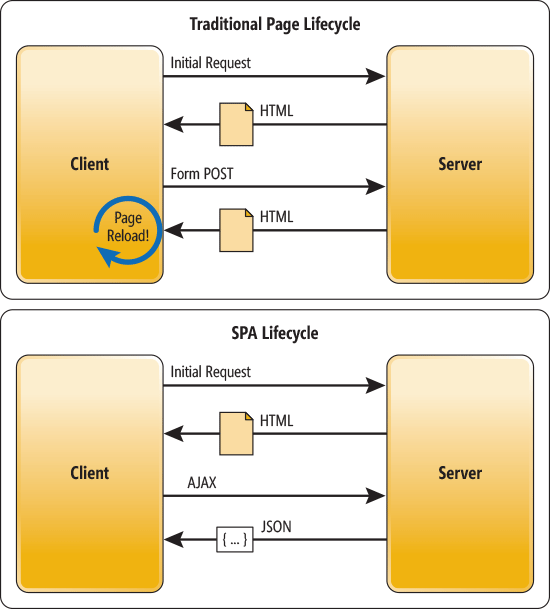
\includegraphics[scale=0.5]{obrazky/spa_vs_traditional}
\par\end{centering}
\caption{Diagram interakce klasické a jednostránkové webové aplikace \cite{spa_diagram}. \label{fig:spa_diagram}}
\end{figure}
\FloatBarrier

\section{Vznik myšlenky SPA}
Původní World Wide Web paradigma vzniklo pro jednoduché zobrazování statických HTML stránek uživateli pomocí webového prohlížeče. Pro stále se zvětšující rodinu webových aplikací je obvyklá představa webu coby sady provázaných hypertextových dokumentů nedostatečná.Ve chvíli, kdy se web začal měnit z \uv{knihovny dokumentů} na aplikační platformu, začala být evidentní potřeba změny tohoto modelu. Možnosti interakce původního HTTP se však omezují na vyžádání jiné webové stránky nebo odeslání formuláře na server k dalšímu zpracování. Takové požadavky uživatelů jsou vždy zpracovávany synchronně, v pořadí v jakém byly doručeny serveru. Každá uživatelská akce způsobí načtení celé nové HTML stránky. Tento princip slavil úspěch díky své jednoduchosti a vedl k masovému rozšíření webových prezentací po celém světě. Aplikace vždy dodržovaly pravidlo rozmístění funkcionality do více stránek, kdy každá stránka odpovídala určitému stavu, události nebo úkolu. Výhody tohoto postupu jsou zřejmé, například uložení jednotlivých stránek do záložek. Naopak nevýhodou může být přenos zbytečně velkých dat, která se posílají stále dokola. Jednoduchost HTTP protokolu, která pomohla rychlému rozšíření, se však později ukázala jako nevhodná pro tvorbu složitejších aplikací. Z jedné strany je jazyk HTML omezující pro webové vývojáře, kteří se musejí omezit na základní možnost úprav klasických formulářů prostřednictvím CSS stylů. Na straně druhé je matoucí pro uživatele, kteří jsou z klasických desktopových aplikací již zvykli na určité prvky a způsob jejich ovladání. Je také velmi neefektivní stahovat ze serveru vždy celou HTML stránku, potřebujeme-li změnit jen nějakou její malou část. V poslední době můžeme pozorovat snahu webových vývojářů příblížit svoje aplikace klasickým desktopovým aplikacím a poskytnout tak uživateli iluzi, že pracuje s běžnou aplikací. Jedná se o tak zvané \textit{jedno-stránkové webové aplikace (Single Page Applications – SPA)} \cite{spa} psané v Javascriptu. V takové aplikaci se veškeré nutné zdroje (kód, média a ostatní) nahrají najednou při načtení úvodní stránky a není již potřeba aplikaci znovu načítat. Veškerá komunikace se serverem se odehrává na pozadí, aniž by rušila dojem uživatele, že pracuje s klasickou desktopovou aplikací. Komunikace má vždy navic asynchronni charakter, který se pro vývoj v Javascriptu typický. Myšlenka tvorby jednostránkých webových aplikací vznikla postupným vývojem skupiny webových technologii, které dnes známe pod zkratkou AJAX. Nejdůležitější z nich, \textit{XMLHttpRequest}, je základní javascriptové rozhraní, které se používá pro asynchronní komunikaci mezi klientem a serverem \cite{xhr}. Komunikace probíhá na pozadí a nedochází při ní k faktickému přenačtení webové stránky. Do širšího povědomí se tyto technologie začaly dostávat kolem roku 2000. Od té doby následoval bouřlivý vývoj, který přinesl nové knihovny a utility, jež zjednodušovali vývoj AJAX aplikací. Nejznámější javascriptovou knihovnou, vzniklou v této době, je dodnes hojně použivané jQuery, které vzniklo v roce 2006. Tato knihovna přináší programátorovi dobře dokumentované rozhraní pro práci se strukturou HTML, asynchronní obsluhu událostí, komunikaci se serverem a podobně. jQuery dnes najdeme téměř na každém webu a jeho alespoň základní znalost je pro každého webového vývojáře takřka nezbytností. Nejednalo se však v té době o jednostránkové webové aplikace, knihovna jQuery sloužila pouze pro řízení některých částí stránky, které komunikovaly se serverem pomocí asynchronních událostí. Využití knihovny pro kompletní obsluhu webové stránky podle princpipu SPA je sice teoreticky možné, avšak v praxi nepraktické. Plné rozvinutí konceptu jednostránkové aplikace umožnil až nástup moderních javascriptových MVC frameworků jako AngularJS nebo ember.js, které vyšly kolem roku 2010. Tyto frameworky adoptovaly návrhový vzor Model – View – Controller (MVC) a výrazně tak usnadňují vývoj webových aplikací, neboť programátoři jsou na tento koncept zvyklí z jiných programovacích jazyků. Speciálně framework AngularJS byl navržen pro snadné použití u Java vývojářů \cite{angular}. Styl vývoje u těchto frameworků byl ve své době revoluční, kompletní logika webové aplikace – získávání a vykreslování dat, validace, nebo routování, se provádí uvnitř webových prohlížečů uživatelů. Proto typická jednostránková aplikace podstatně méně zatěžuje server. Server pouze poskytuje data a reaguje na událostí, tvoří tedy takzvané API. Zobrazování UI a veškeré interakce s uživatelem řídí Javascript \cite{spa_horyna} \cite{spa}. 

\section{Princip technologie}
Základním principem jednostránkových aplikací je spuštění celé webové aplikace při prvním načtení vstupního bodu aplikace, většinou se jedná o soubor index.html. S prvním přístupem jsou načteny všechny základní zdroje definované v hlavičce HTML dokumentu. Další zdroje jsou načítány až ve chvíli, kdy jsou skutečně potřeba, i tak je ale při prvním načtení nutné stáhnout a zpracovat velké množství dat. To je jedna z nevýhod jednostránkových webových aplikací. Stahování dalších dat nebo HTML šablon je plně v režii frameworku použitého pro vývoj. Komunikace probíhá pomocí technologie XHR, dle principu AJAX. Pomocí Javascriptu je ze serveru stažen další obsah (multimédia, HTML kód nebo text), ten je načten do paměti prohlížeče a dojde k plynulému překreslení nějaké části aplikace. Pomocí této techniky je možné měnit obsah uživateli \uv{pod rukama}, aniž bychom museli znovu načíst a vykreslit celý dokument, jak by bylo nutné u klasických webových aplikací. Stejným způsobem mohou být načítány i CSS soubory, nebo další javascriptové zdroje. U SPA běží celá aplikace uvnitř webového prohlížeče, kompletní aplikační logika je definována v Javascriptu a server je redukován na poskytovatele dat pomocí REST API. Hovoříme tedy o takzvaném \uv{tlustém klientu}. Možnost běhu celého aplikace pomocí javascriptového jádra webového prohlížeče umožnil jejich masivní vývoj posledních let a s ním spojený významný nárust jejich výkonnosti. Spuštění celé jednostránkové aplikace však značně zatěžuje procesor koncového zařízení, což je problém především u některých mobilních zařízení, které mají méně výkonné procesory. Následující diagram dobře ilustruje rozdělení rolí typické jednostránkové aplikace naprogramované v jazyce Javascript \cite{spa_book} \cite{spa_web}.

\begin{figure}[h]
\begin{centering}
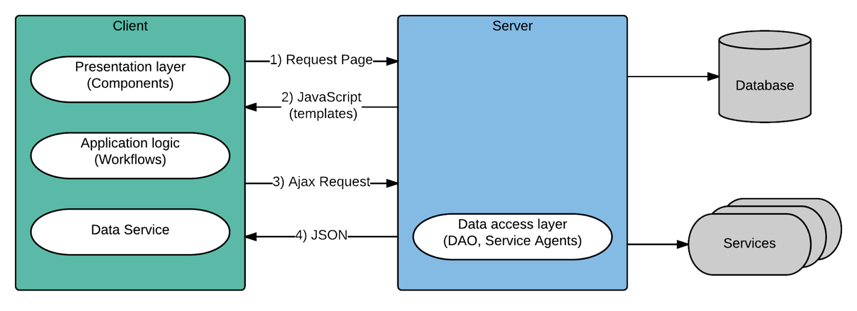
\includegraphics[scale=1]{obrazky/spa_architecture}
\par\end{centering}
\caption{Diagram typické architektury jednostránkové webové aplikace v javascriptu \cite{isomorhic_book} \label{fig:spa_architecture}}
\end{figure}

\section{Hlavní výhody}
Obecně se tato technologie hodí převážně pro weby, které počítají s velkou mírou interaktivity, mají tedy určitou logiku, kterou je nutné vyhodnocovat v prohlížeči. Prakticky se ale jako SPA dá naprogramovat jakákoliv webová aplikace, od statických prezentací až po velké informační systémy. Většina webových aplikací je dnes navrhována s ohledem na vysokou interaktivitu. Použití Javascriptu je proto u webových aplikací prakticky nutností. Veškerá datová komunikace probíhá pomocí AJAX, tento způsob se využívá také při \textit{lazy loadingu}, který obsah stránky vykreslí v několika krocích. U náročných stránek tím lze docílit rychlého zobrazení nejdůležitějšího obsahu, další méně důležité části lze načíst až později. Díky vysokému zapojení Javascriptu lze dnes většinu jednostránkových aplikací alespoň částečně používat také offline \cite{spa_book} \cite{spa_horyna}.

Následující kapitola shrnuje hlavní výhody jednostránkových webových aplikací, spolu se souvisejícími technologiemi, které je realizují.

\subsection{Větší míra interakce}
Standard HTML zná pouze několik základních vstupních prvků (tlačítka, textová pole, výběrové seznamy, zaškrtávací pole a další), pomocí kterých je realizována interakce uživatele s webovou aplikací. Větší míra zapojení Javascriptu umožňuje rozšířit tuto základní nabídku prvků, čímž je zlepšena intuitivnost a uživatelský prožitek (user experience) webové aplikace. Jako příklad lze uvést dialogová okna, funkci \textit{drag and drop}\footnote{Vyvolání nějaké akce přetáhnutím souboru do webového prohlížeče.}, nebo rozšířené formulářové prvky například pro výběr datumu či barvy. Také možnost využití přechodů nebo animací může zlepšit uživatelský prožitek \cite{spa_book} \cite{spa_horyna}.

Jednostránková javascriptová aplikace přestavuje takzvanou RIA (Rich Internet Application). Taková aplikace by se dala definovat jako webová aplikace, která se snaží nabídnout některé prvky klasických desktopových aplikací \cite{ria}. Mnoho z těchto nových prvků přináší standard HTML5, jenž je dnešními webovými prohlížeči velmi dobře podporován\cite{spa_book} \cite{spa_web}. HTML5 je nový standard značkovacího jazyka HTML vydaný v roce 2014, který přinesl \cite{janovsky_html5} \cite{html5_css3_book}:

\begin{itemize}
\item nové sémantické elementy: <article>, <aside>, <details>, <figcaption>, <figure>, <footer>, <header>, <main>, <mark>, <nav>, <section>, <summary>, <time>,
\item nové druhy vzhledu a chování formulářových polí <input>,
\item nový tag <datalist> pro výběr z více možností,
\item validaci formulářů a některé užitečné atributy formulářových polí, například placeholder,
\item tagy <video> a <audio>,
\item atribut download k odkazům vynucující stažení a určující jméno, souboru
\item lokální datová úložiště (asociativní pole, relační databáze), které je ale nutné obsluhovat Javascriptem,
\item javascriptem dostupná API na geolokaci, drag \& drop, web workers a SSE zjednodušení zápisů doctype a kódování stránky\
\item a mnohá další.
\end{itemize}

Lepší možnosti interakce přinesl do webových prohlížečů také nový standard stylovacího jazyka CSS. Verze CSS3 byla vydána konsorciem W3C (World Wide Web Consortium) v roce 2015 a dnes se dokončuje jeho implementace do webových prohlížečů \cite{css3} \cite{html5_css3_book}. Třetí verze přinesla především tyto novinky.

\begin{itemize}
\item \textbf{Media queries} – Umožňují aplikovat některé CSS deklarace jen po splnění určitých podmínek, většinou typu zobrazení a velikost rozlišení. Media queries je jedním ze tří pilířů responzivního webdesignu, spolu s fluidním layoutem a fluidními médii. Příklad použití: \textit{@media screen and (min-width : 500px) {h1 {color: blue}}} nastaví všem nadpisům modrou barvu, ale jen na rozlišení větší než 500px na šířku. 
\item \textbf{Nové selektory }např.: nth-child() , :nth-of-type(), checked().
\item \textbf{Vícesloupcový layout.}
\item \textit{Oblé rohy} – vlastnost border-radius dokáže definovat \uv{kulatost} rohů.
\item \textbf{Stínování} – vlastnost box-shadow přijímá čtyři parametry: horizontální posunutí stínu, vertikální posunutí stínu, okraj stínu a jeho barvu.
\item \textbf{Průhlednost} – pomocí vlastnosti opacity lze zprůhlednit jakýkoliv HTML objekt na stránce.
\item \textbf{CSS3 transformace} – vlastnost transform umožňuje změnu orientace, tvaru, perspektivy i velikosti objektů tedy různé přetáčení, překlápění nebo škálování.
\end{itemize}

Samotnou vysokou interaktivitu ale umožňuje především samotný Javascript, který realizuje veškeré DOM manipulace, na kterých je celá jednostránková aplikace založena \cite{spa_book} \cite{spa_web}. 

\subsection{Obnovování pouze určitých částí aplikace}
Jednou z velkých novinek moderních webových aplikací bylo odstranění nutnosti načítat a zobrazovat celou HTML stránku znovu při každé uživatelské akci. Neustálé čekání na načtení stránky může na uživatele působit rušivě a kazit jeho celkový dojem. Jednostránková webové aplikace v Javascriptu je kompletně načtena do prohlížeče při první návštěvě aplikace a veškerá další komunikace, přechody mezi stránkami nebo validace vstupních dat probíhají bez opakovaného načítání celé stránky. Díky tomuto chování bylo možné webové aplikace přiblížit k těm desktopovým, změny v aplikaci probíhají téměř v reálném čase a daná webová aplikace je tak uživatelsky přívětivější \cite{spa_book} \cite{spa_web}.

\subsection{Mohou běžet offline}
SPA lze implementovat i tak, aby bylo možné s ní omezeně pracovat i v době krátkodobé nedostupnosti internetového připojení. Změny provedené uživatelem v offline režimu se ukládají do některé z pamětí webového prohlížeče. Dobře se k tomu hodí nové HTML5 komponenty \textit{Application Cache} nebo \textit{Local Storage}. Ty umožňují ukládát stav aplikace do paměti prohlížeče nebo dokonce ukládat soubory na disk klientského počítače. V okamžiku navázání spojení dojde k odeslání lokálně uloženého stavu celé aplikace na webový server, tedy ke zpracování všech akcí, které uživatel provedl ve stavu offline \cite{spa_book} \cite{spa_web}.

\subsection{Lepší výkonnost}
Díky využití výpočetního výkonu webového prohlížeče pro obsluhu vykreslování a základních uživatelských akcí nejsou kladeny takové nároky na webový server. Obecně lze řici, že díky zapojení javascriptu pracuje jednostránková webová aplikace rychleji než klasická webová aplikace. Je to především proto, že se datová komunikace omezuje jen na nezbytně nutná data a veškeré obslužné operace probíhají na pozadí uvnitř webového prohlížeče, ale také díky přenesení zodpovědnosti za vykreslování HTML z webového serveru do prohlížeče. Díky protokolu Websocket lze komunikaci aplikace se serverem ještě zrychlit a optimalizovat \cite{spa_book} \cite{spa_web}.
\pagebreak

\section{Roztříštěnost koncových zařízení}
Moderní doba přinesla obrovskou škálu zařízení, pomocí nichž lze přistupovat na Internet. Internet se stále více posouvá z osobních počítačů do každodenního života. Jak je vidět na grafu \hyperref[fig:mobile_popularity]{3.3} používání internetu na mobilních zařízeních v posledních několika letech velmi stoupá \cite{mobile_popularity}. 

\begin{figure}[h]
\begin{centering}
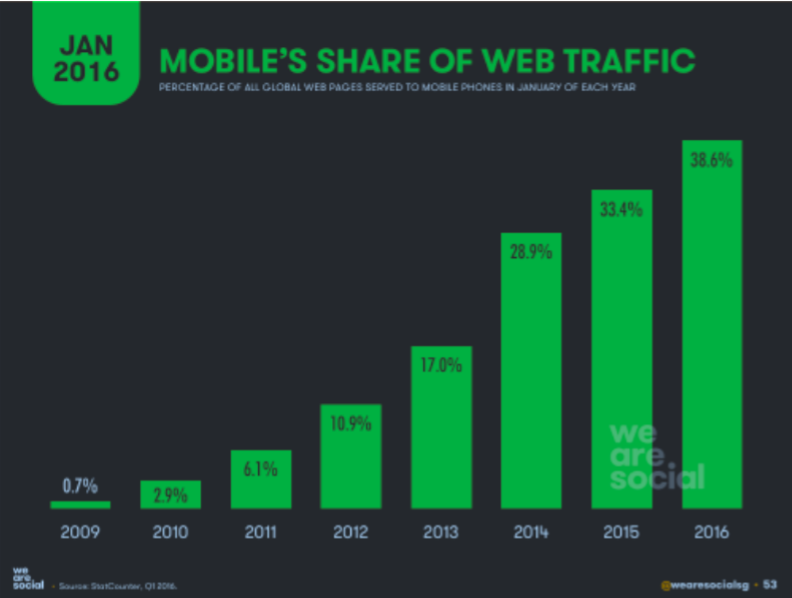
\includegraphics[scale=0.4]{obrazky/mobile_popularity}
\par\end{centering}
\caption{Vývoj zastoupení mobilních uživatelů na webu mezi lety 2009-2016 \cite{mobile_popularity}. \label{fig:mobile_popularity}}
\end{figure}
\FloatBarrier

Nástup mobilního internetu zvyšuje požadavky na návrh uživatelských rozhraní, která musí být schopná upravit zobrazení v závislosti na dostupném prostoru. Jak ukazuje obrázek \hyperref[fig:resolutions]{3.4} větší škála koncových zařízení přináší obrovské množství různých rozlišení. V praxi je nutné testovat web alespoň na klasickém počítači, mobilním telefonu a tabletu. Hovoříme tedy o takzvaném \uv{responzivním designu}. Jeho hlavní oblastí je adaptivní HTML layout. Je ale také nutné řešit rozdíly mezi javacriptovými jádry mobilních prohlížečů \cite{responsive_design}. Sjednocení běhových prostředí javacriptu se realizuje pomocí externích knihoven zvaných polyfillů, nejpoužívanější z nich je \textit{Modernizr}, který vedle doplnění nepodporovaných funkcí, poskytuje také rozhraní pro detekci novějších vlastností Javascriptu. Nedostupné funkce potom můžeme simulovat a tím zvýšíme kompatibilitu celé aplikace \cite{modernizr}.

\begin{figure}[h]
\begin{centering}
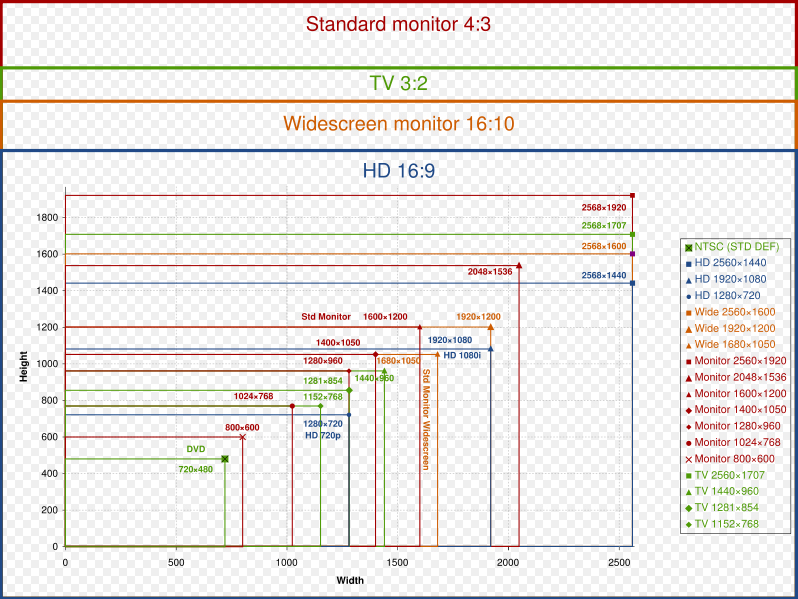
\includegraphics[scale=0.4]{obrazky/resolutions}
\par\end{centering}
\caption{Nejčastější rozlišení koncových zařízení na internetu \cite{mobile_popularity}. \label{fig:resolutions}}
\end{figure}
\FloatBarrier

\section{Vhodné knihovny}
Celý vývoj jednostránkových webových aplikace je hluboce založen na použití knihoven. Dobrý přehled poskytuje web TodoMVC \cite{todomvc}, kde je možné nalézt implementace jednoduchého úkolovníku ve většině javascriptových MVC frameworků. Mezi knihovny, které jsou pro SPA vhodné, patří například AngularJS, který představuje celý MVC framework, řeší tedy veškerou aplikační logiku uvnitř webového prohlížeče. Podobně orientované jsou také frameworky Backbone.js a Ember.js. Zatímco dnes popularní React se soustředí pouze na generování pohledu (view), tedy v našem případě cílového HTML kódu \cite{react}. Tento framework se nejčastěji používá jako zobrazovací vrstva u isomorfních aplikací a je také součástí ukázkové aplikace popsané v praktické části práce \cite{spa} \cite{spa_book}.

\vspace{0.3cm}
\noindent Některé často používané MVC frameworky:
\begin{itemize}
\item AngularJS,
\item BackboneJS,
\item EmberJS,
\item SpineJS,
\item SammyJS,
\item Knockout.js,
\item batman.js,
\item canjs.
\end{itemize}

\section{Nevýhody a časté problémy při vývoji}
Často zmiňovanou nevýhodou technologie jednostránkových aplikací je absolutní závislost na Javascriptu, který některá zařízení nemusí podporovat. Ačkoli podíl těchto zařízení stále klesá, problémem jsou především vyhledávací roboti. Mezi další nevýhody SPA patří \cite{spa_horyna}:

\begin{itemize}
\item časově, datově a výpočetně náročné první načtení webové aplikace, které je dané dobou načítání všech javascriptových zdrojů a dobou jejich zpracování jádrem webového prohlížeče,
\item celá aplikace se poskládána dynamicky, vyhledávací roboti (a uživatelé s vypnutým Javascriptem) jí mohou špatně zobrazit,
\item složitější implementace kvůli nutnosti správy aplikačního stavu,
\item problém s historií a tlačítkem zpět,
\item obrovské množství použitelných knihoven, problém vhodného výběru,
\item složitější příprava vývojového prostředí.
\end{itemize}

Jednou z problematických oblastí je také reakce jednostránkové aplikace na použití tlačítka zpět a obecně práce s URL a historií prohlížení. Tento problém se podařilo vyřešit až s rozšířením možností javascriptového API pro řízení historie a URL prohlížeč. Především velmi pomohlo doplnění možnosti ukládání stavu aplikace do historie prohlížeče. Jedná se o příkaz \textit{history.pushState()}. Pomocí něj lze zajistit stejné fungování historie jako u běžných serverových webových aplikací. Moderní javascriptové frameworky toto dnes řeší automaticky \cite{spa_book}.

Vyřešit problém špatné indexovatelnosti jednostránkových aplikací je mnohem složitější. Díky konceptu vykreslení celé aplikace pomocí Javascriptu, neexistuje jednoduché řešení, jak vyhledávacím robotům umožnit korektní zobrazení aplikace. Jedním z používaných řešení je spuštění takzvaného \uv{headless browseru}, tedy plnohodnotného webového prohlížeče bez grafického uživatelského rozhraní. Ten potom naslouchá na určené speciální URL, zpracuje celo jednostránkovou javascriptovou aplikaci a vrátí robotům kompletní HTML. Společnost Google doporučuje používat takzvanou \uv{hashbang notaci} 
( \#!aktualni-url) pro definici URL aplikace. Vyhledávací robot Googlu se potom pro adresu například 
\textit{www.example.com/\#!items/0/detail} pokusí získat její obsah na 
\textit{www.example.com/?\_escaped\_fragment=items/0/detail}, kde naslouchá zmiňovaný headless browser, který vrátí obsah pro vyhledávač \cite{google_crawler}. Celý proces ilustruje obrázek 
\hyperref[fig:prerender]{3.5}. Spuštění celého webového prohlížeče na serveru je ale velmi neefektivní a celé řešení vyžaduje složitou konfiguraci. Existují také externí služby, které vykreslování jednostránkových javascriptových aplikací pro vyhledávací roboty řeší, můžeme zmínit například Prerender.io \cite{prerender}. 

\begin{figure}[h]
\begin{centering}
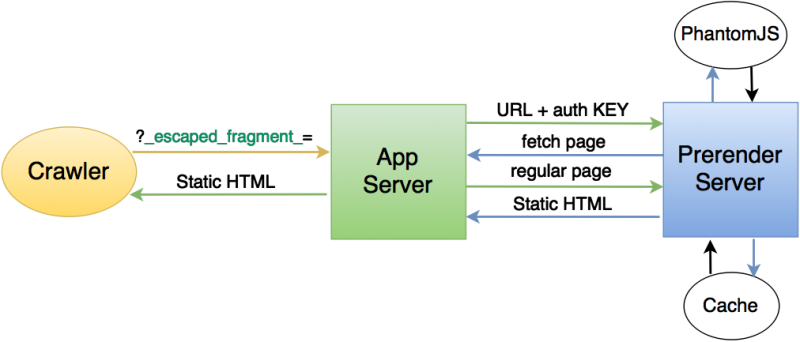
\includegraphics[scale=0.4]{obrazky/prerender}
\par\end{centering}
\caption{Diagram komunikace vyhledávacího robota s headless prohlížečem \cite{crawler_spa}. \label{fig:prerender}}
\end{figure}
\FloatBarrier

Mnohé z výše uvedených problémů řeší koncept isomorfních webových aplikací, který rozšířuje koncept SPA přenesením některých pravomocí zpět na webový server, který je také poháněn jazykem Javascript. Isomorfismus v kontextu webových aplikací znamená použití stejného jazyka pro server i webový prohlížeč \cite{universal_js}.

\chapter{Isomorfní přístup k programování webových aplikací}
\label{sec:isomorphic}
Při startu nového projektu je v první řadě nutné navrhnout vhodnou architekturu a s ní související technologická řešení. U větších projektů se dnes stále častěji uvažuje o architektuře jednostránkových aplikací, které jsou dnes velmi populární. Mají ovšem několik podstatných nevýhod, jednou z hlavních je špatná indexovatelnost vyhledávači, jež je nevýhoda, která přímo vyplývá z návrhu, je tedy velmi těžké jí odstranit. Roboti internetových vyhledáváčů totiž většinou neovládájí Javascript a nedokážkou proto webové aplikace korektně zobrazit. Další nevýhodou běžných SPA je náročnost javascriptového kodu celé aplikace pro webový prohlížeč v mobilním telefonu, načítání jednostránkových aplikací často trvá příliš dlouho, což kazí celkový dojem uživatele \cite{spa} \cite{spa_book}. 

Mnohé z těchto nevýhod řeší takzvaný isomorfní přístup, který v oblasti programování webových aplikací znamená použití stejného programovacího jazyka pro backend\footnote{serverová část aplikace} i frontend\footnote{klientská část aplikace (webový prohlížeč)}. Poprvé s tímto pojmem přišel Charlie Robbins v roce 2011 ve svém článku \textit{Scaling Isomorphic Javascript Code} \cite{isomorphic_founder}, kde popisoval isomorfismus jako schopnost použití stejného kódu pro server i webový prohlížeč. Jediným jazykem, který lze dnes takto použít je Javascript. Tento přístup poté popularizoval Spike Brehm v roce 2013 v článku \textit{Isomorphic Javascript: The Future of Web Apps} \cite{isomorphic_airbnb2}.

Isomorfismus je obecně pojem pro zobrazení mezi dvěma matematickými strukturami, které je vzájemně jednoznačné a zachovává všechny vlastnosti touto strukturou definované. Jinými slovy, každému prvku první struktury odpovídá právě jeden prvek struktury druhé a toto přiřazení zachovává vztahy k ostatním prvkům \cite{isomorphic_def}. Pojem lze dobře vizualizovat pomocí grafů, na obrázku \hyperref[label:isomorphic_graph]{4.1} jsou dva vzájemně isomorfní grafy.

\begin{figure}[h]
\begin{centering}
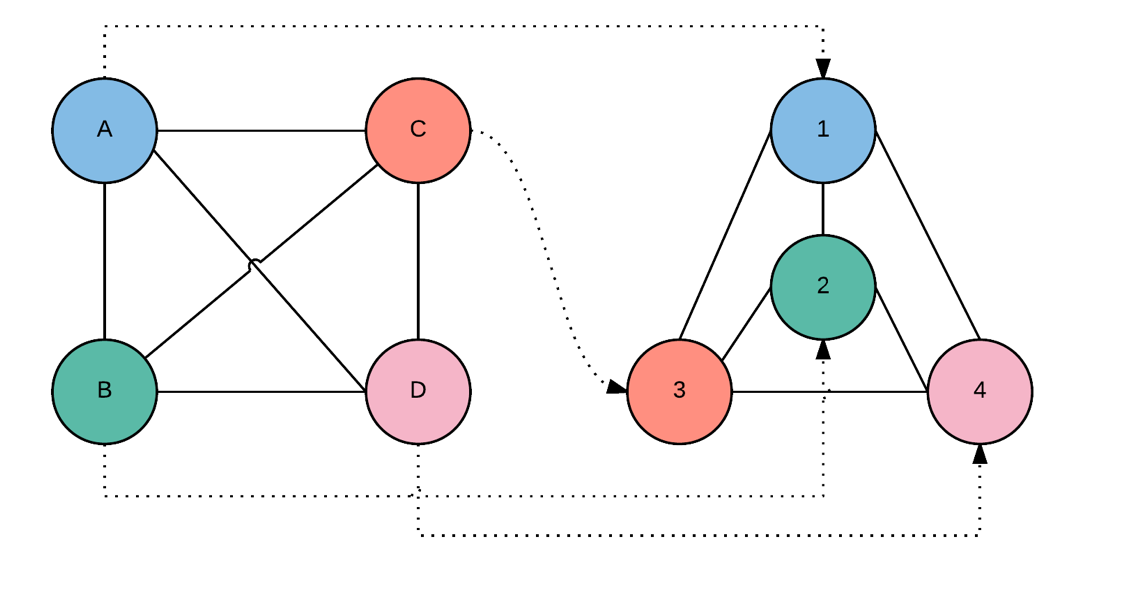
\includegraphics[scale=0.5]{obrazky/isomorphic_graph}
\par\end{centering}
\caption{Dva vzájemně isomorfní grafy \cite{isomorhic_book} \label{fig:isomorphic_graph}}
\end{figure}
\FloatBarrier

Isomorfní webová aplikace\footnote{V době dokončování této práce bylo komunitou rozhodnuto o používání názvu \textit{univerzální webové aplikace} \cite{universal_js}. V této práci se budu držet původního termínu isomorfní.} je ze své podstaty také jednostránkovou aplikací, která ovšem mnohem více zapojuje serverovou část. Ta je u klasických jednostránkových aplikací redukována na servisní vrstvu a datové API. Takto navržené aplikace používají stejný javascriptový kód pro webový prohlížeč i webový server, což má pro vývoj několik zajímavých důsledků \cite{isomorhic_book}:

\begin{itemize}
\item vývojáři udržují jen jeden hlavní projekt (codebase),
\item isomorfní web částečně funguje i bez Javascriptu,
\item možnost používání stejných knihoven pro server i prohlížeč.
\end{itemize}

Takto navržené webové aplikace začínají být velice populární. Příkladem je hlavně Facebook nebo třeba Airbnb \cite{isomorphic_airbnb} \cite{isomorphic_airbnb2}, Netflix \cite{netflix} nebo nová verze Uber. Dnes existuje mnoho knihoven pro vývoj isomorfních webových aplikací, některé z nich vznikly ve společnosti Facebook, jako výsledek složitého vývoje sociální sítě. Nejzásadnější z nich, framework React přinesl zcela nový pohled na návrh a implementaci uživatelských rozhraní. Také oblíbená architektura Flux, která přináší sjednocení práce s daty aplikace, vznikla ve stejné společnosti \cite{flux}. Mnoho existujících javascriptových knihoven pro prohlížeč jako Underscore, Backbone.js, Handlebars.js, Moment nebo jQuery, je možné používat také na serveru s nulovými nebo minimálními úpravami \cite{isomorphic_airbnb2}.

\section{Výhody isomorfního přístupu}
Isomorfní přístup k programování webových aplikací je výsledek více než dvaceti let evoluce v tomto oboru. Princip využívá interaktivity a uživatelské přívětivosti klasických jednostránkových webových aplikací v Javascriptu, které rozšířuje a vylepšuje pomocí většího zapojení serveru. Isomorfní přístup také řeší většinu nevýhod klasických webových aplikací. Například díky možnosti vykreslování šablon na straně serveru řeší problém indexace běžných SPA. Vyhledávací robot bez Javascriptu uvidí stejný web jako běžný uživatel s Javascriptem \cite{isomorhic_book}. Následující kapitola popíše hlavní výhody isomorfismu spolu s řešením častých problémů jednostránkových webových aplikací.

\subsection{Sjednocení používaného jazyka a prostředí}
První a nejdůležitější výhodou a sjednocení používaného jazyka, jinými slovy možnost použití Javascriptu pro prohlížeč i server. Isomorfní aplikace kvůli principu sdílení kódu zpravidla používají dokonce jeden projekt pro obě prostředí. Vždy ale bude existovat nějaká logika určená jen pro prohlížeč nebo jen pro server. Podle doporučovaných konvencí je proto vhodná rozdělit isomorfní aplikaci na tři základní adresáře: \textit{client}, obsahující kód pouze pro prohlížeč, \textit{server} s kódem určeným pro server a \textit{common}, který obsahuje sdílený kód \cite{isomorhic_book}.

Dva následující obrázky dobře ilustrují rozdíly mezi architekturami běžných a isomorfních SPA \cite{codepicnic_universaljs}.
\begin{figure}[h]
\begin{centering}
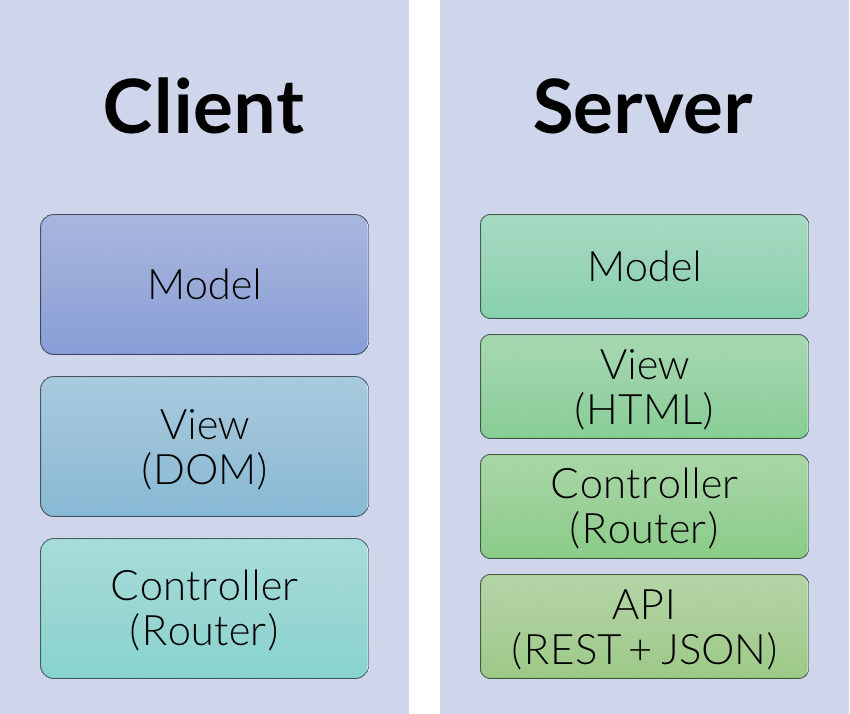
\includegraphics[scale=0.5]{obrazky/classic_webpage_architecture}
\par\end{centering}
\caption{Diagram architektury typické jednostránkové webové aplikace \cite{codepicnic_universaljs} \label{fig:classic-web-arch-diagram}}
\end{figure}

Jak je vidět na diagramu výše, SPA podle původního konceptu přesunulo většinu zodpovědnosti z serveru na klienta, uvnitř webového prohlížeče probíhá vykreslování šablon, routování požadavků a další věci, které dříve vždy řešil server. Při vzniku SPA to bylo považováno za výhodu, díky snížení nároků na webové servery \cite{spa_book}. Redukce serverové části aplikace na datové API však přinesla také mnohé nevýhody, jednostránková aplikace byla mnohem výpočetně náročnější než běžná webové aplikace, indexovatelnost a obecně SEO bylo problémem. Po několika letech boomu jednostránkových aplikací se tak začaly objevovat názory, že je nutné některé věci přesunout zpět na webový server. V této době byla již velmi používaná platforma node.js, bylo tedy možné napsat i serverovou část aplikace v Javascriptu a tím používat stejný jazyk pro obě prostředí. Isomorfní webová aplikace tedy používá pouze jazyk Javascript, pro klient i server. Typicky serverové problémy, jako vykreslování šablon nebo routování požadavků byly přesunuty zpět na na stranu serveru \cite{isomorhic_book}.
\begin{figure}[h]
\begin{centering}
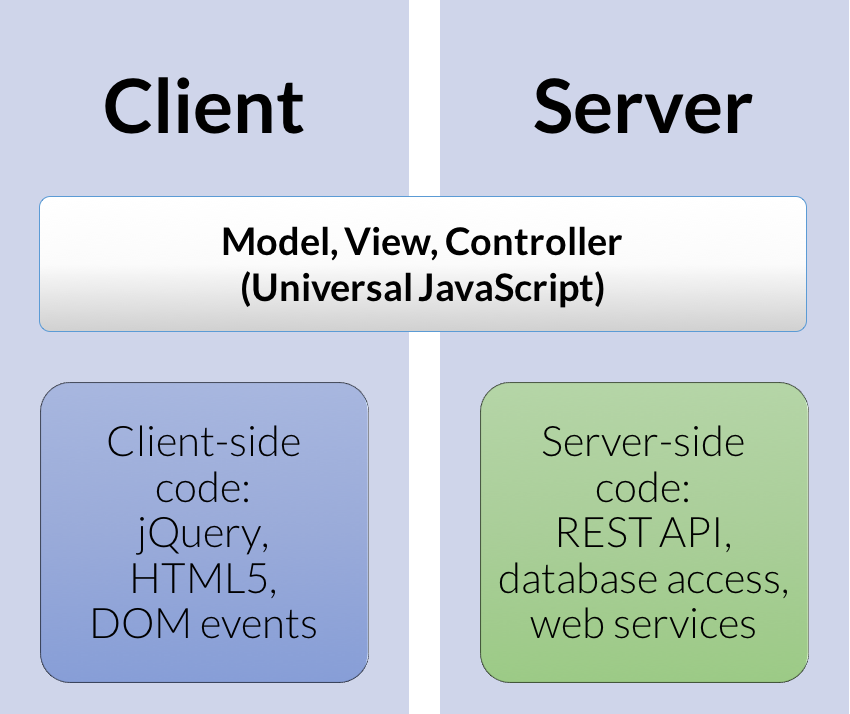
\includegraphics[scale=0.5]{obrazky/isomophic_webpage_architecture}
\par\end{centering}
\caption{Diagram architektury isomorfní webové aplikace \cite{codepicnic_universaljs} \label{fig:isomophic-web-arch-diagram}}
\end{figure}
\FloatBarrier

\subsection{Interaktivita jednostránkových aplikací}
I isomorfní webová aplikace je pořád jednostránkovou webovou aplikací, se všemi jejími výhodami. Veškeré interakce s uživatelem probíhají asynchronně bez dalšího načítání nové stránky. Server řídí routování požadavků a vykreslování stránek a to buď přímo při prvním načtení aplikace nebo pomocí AJAX při procházení navigace. Koncept isomorfních webových aplikací vylepšuje koncept SPA rozšířením kompetencí webového serveru a zároveň tím řeší největší problémy jednostránkových webových aplikací \cite{isomorhic_book}.

\subsection{Sdílení kódu mezi prostředími}
Obvykle nejčastěji zmiňovanou výhodou isomorfních webových aplikací je možnost sdílení zdrojového kódu. Možnost sdílení kódu mezi prohlížečem a serverem přináší určitá specifika, na které je nutné při vývoji isomorfních webových aplikací myslet. Zejména je nutné vyhnout se používání rozhraní, které je specifické pro dané běhové prostředí, například objekt \textit{window} v prohlížeči, nebo \textit{env} v node.js. Místo toho je nutné používat obslužné metody isomorfního frameworku, který zapouzdřuje tyto specifická rozhraní a umí je dle prostředí přízpůsobit. Tento přístup je nazývá \textit{environent-agnostic} a definuje tvorbu univerzálně použitelného Javascriptu, který správně funguje na všech prostředích \cite{isomorhic_book} \cite{codepicnic_universaljs}.

Je tedy možné sdílet mnoho použitého kódu, například šablony nebo validační pravidla, některé části aplikace, jako například router, je ale nutné implementovat zvlášť pro server a pro prohlížeč. Části, které je nutné zdvojit, však většinou není nutné udržovat na dvou místech, moderní isomorfní devstacky dokážou tyto procesy automatizovat. Například u routovacích pravidel se použitý task runner při spuštění aplikace postará o distribuci pravidel do serverového i klientského routeru \cite{isomorhic_book} \cite{codepicnic_universaljs}.

\vspace{3mm}
\noindent Následující ukázka kódu ilustruje implementaci funkce suma pro webový prohlížeč, server v node.js a její univerzální variantu. Ta používá IIFE (viz. \hyperref[sec:variable_scope]{2.2.2}), jež dostane jako parametr nejvyšší globální objekt daného prostředí. Tedy \textit{window} v případě prohlížeče a \textit{exports} v případě node.js.
\begin{lstlisting}[language=Javascript,caption={Ukázka principu enviroment-agnostic, tedy JS kódu nezávislého na běhovém prostředí}]
// Javascript v prohlížeči
function browserSum(a,b){
		return a+b;
}

// node.js
module.exports.serverSum = function(a,b){
		return a+b;
};

// univerzální Javascript (environment-agnostic)
(function(exports){
     exports.isomorphicSum = function(a,b){
     		return a+b;
     };
})(typeof exports ? exports : window);
\end{lstlisting}

Při použití vhodných nástrojů nemusí programátor nad nezávislostí kódu přemýšlet, řeší ji automaticky použitý framework. Také systém modulů, který přinesl Javascript ES6, pomáhá univerzálnosti javascriptového kódu.

\subsection{Rychlejší prvotní načtení aplikace}
Běžné jednostránkové aplikace se při prvním načtení kompletně nahrají do prohlížeče a spustí. Tohle prvotní načtení je ale většinou velmi náročné na zdroje i výpočetní výkon. Javascriptové jádro webové prohlížeče musí stáhnout a zpracovat všechny javascriptové soubory, načíst HTML šablony a celou aplikaci včetně všech dynamických prvků spustit. To může trvat i několik sekund. Server poskytuje jen čisté HTML, které většinou neobsahuje žádný text, ale jen definice všech zdrojů aplikace pomocí HTML značek \textit{script} nebo \textit{rel}. Naproti tomu isomorfní aplikace vrátí na první načtení již vykreslenou úvodní stránku, definice externích zdrojů jsou zastoupeny v mnohem menší míře, jelikož výpočetně náročné části řeší server \cite{isomorhic_book} \cite{codepicnic_universaljs}. Na následujícím grafu je dobře vidět rozdíl časů prvního načtení klasické jednostránkové aplikace postavené na velkém MVC frameworku a té využívající isomorfní přístup s pomocí frameworku React \cite{spa_perf}. 
\begin{figure}[h]
\begin{centering}
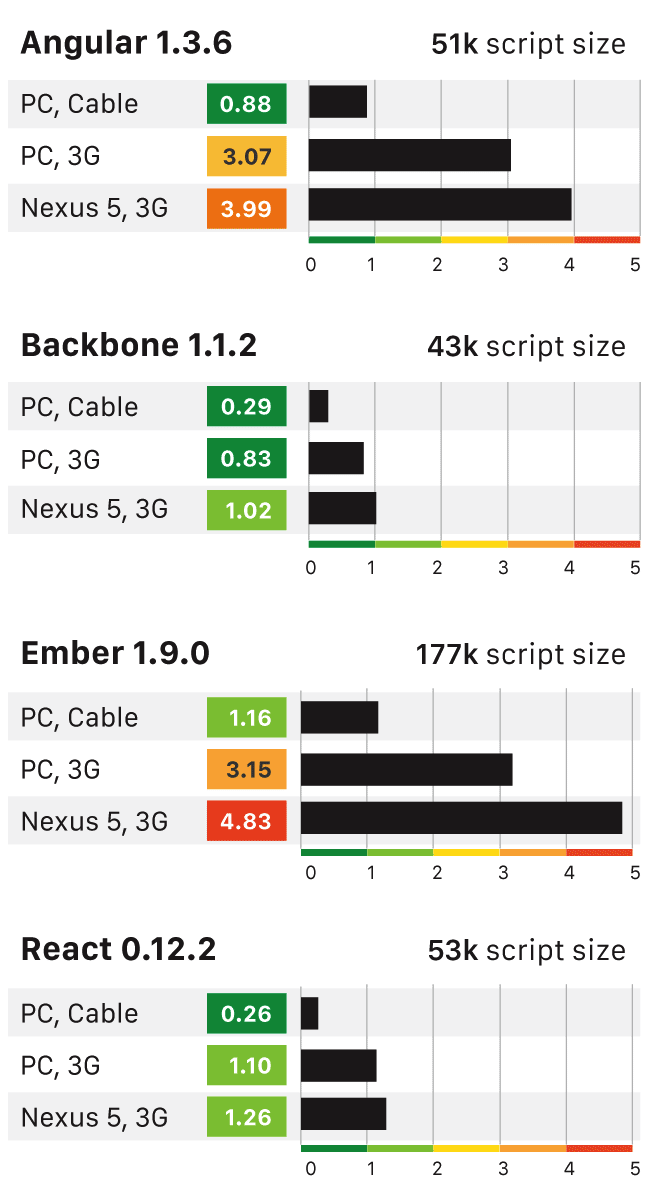
\includegraphics[scale=0.2]{obrazky/first_render_times}
\par\end{centering}
\caption{Graf časů prvotního načtení Javascriptových frameworků \cite{spa_perf} \label{fig:first_load_times}}
\end{figure}
\FloatBarrier

Jak je vidět, čas prvního načtení isomorfní aplikace využívající React je především díky serverovému vykreslování výrazně nižší. Také tolik nezáleží na výkonu koncového zařízení, isomorfní aplikace je stejně rychlá na mobilních telefonech jako v osobních počítačích \cite{isomorhic_book} \cite{codepicnic_universaljs}. 

\subsection{Indexovatelnost vyhledávači}
Známé javascriptové frameworky pro tvorbu běžných jednostránkových aplikací, jako například AngularJS, mají velký problém s indexovacími roboty vyhledávačů. Robot, který prochází Internet většinou nepodporuje Javascript, tím pádem se mu jednostránková aplikace, která plně běží v prohlížeči uživatele, nespustí. Vyhledávač potom nevidí strukturu ani obsah takové aplikace. Existuje několik řešení, pomocí kterých lze tento problém řešit. Jedna z možností je provozování celého webového prohlížeče uvnitř serveru v takzvaném headless (bezešvém) módu. Tento integrovaný prohlížeč potom zpracovává javacriptovou aplikaci na straně serveru a vyhledávacím robotům vrací kompletně vykreslenou stránku v čistém HTML, se kterou již indexační robot nemá nejmenší problém. Běžnjá isomorfní aplikace ale částečně vykresluje HTML na serveru, vyhledávácí roboti tak obdrží mnohem bohatší stránku než u klasických SPA. Tomuto přístupu se říká \textit{server-side rendering} \cite{isomorhic_book} \cite{codepicnic_universaljs}.

\subsection{Server-side rendering}
\label{sec:server_side_rendering}
Server-side rendering umožňuje vykreslovat javascriptové šablony na straně serveru a vracet je webovému prohlížeči už částečně zpracované. Tuto možnost přinesla platforma node.js, která je schopná používat většinu javascriptových frameworků, které jsou určeny pro prohlížeč. Díky tomu můžeme vykreslovat šablony na serveru naprosto ekvivalentně jako v prohlížeči, což je stěžejní část isomorfního přístupu. Ten používá server-side rendering jen při prvním načtení aplikace, další operace jsou již plně v režii webového prohlížeče. To znamená, že se stránka korektně zobrazí i vyhledávacím robotům nebo uživatelům s vypnutým Javascriptem. Server-side rendering tedy řeší jednu z často zmiňovaných nevýhod klasických jednostránkových aplikací. Tento přístup také podstatně zrychluje první načtení aplikace, není totiž nutné čekat na stažení a zpracování veškerého javascriptového kódu prohlížečem \cite{isomorhic_book} \cite{codepicnic_universaljs}.

\subsection{Vývoj mobilních aplikací}
Vzhledem k tomu, že je celá isomorfní aplikace naprogramována v Javascriptu, lze jí provozovat v každém webovém prohlížeči, včetně toho v mobilním telefonu. V mobilu lze webový prohlížeč spustit také bez uživatelského rozhraní (adresní řádek a podobně) a simulovat tím dojem nativní aplikace. Lze potom vyvíjet mobilní aplikaci v HTML, CSS a Javascriptu, která bude při správném nastylování prakticky k nerozpoznání od té nativní. Výhodou webových aplikací je nenáročnost na prostor, aplikace je včetně svých dat uložena na vzdáleném serveru, kde probíhají i některé výpočty. To usnadňuje také aktualizace, stačí pouze nahrát novou verzi na server. Pomocí frameworku Apache Cordova \cite{cordova}, je možné javascriptovou aplikaci distibuovat standardními prodejními kanály jako běžné aplikace. Zabalená aplikace jako první krok nastartuje webový prohlížeč mobilního zařízení a následně se v něm spustí. Aplikace je pak vytvořena jenom jednou a potom s drobnými úpravami vydána pro různé mobilní platformy. Některé frameworky podporující tvorbu mobilních aplikací v Javascriptu, poskytují také připravené grafické motivy, které reprezentují jednotlivé mobilní platformy. Stejné aplikace potom vypadá jinak na systému iOS a jinak na Androidu, vždy s ohledem na grafický styl dané platformy \cite{mobile_apps}. Tyto motivy nabízí například Ionic \cite{ionic}.

\section{Reaktivní programování}
Důležitým konceptem isomorfního přístupu je aplikování reaktivního programování. Jeho základním principem je vytváření celého uživatelského rozhraní znovu s každou provedou změnou. Dalším důležitým aspektem je princip komunikace pouze pomocí událostí. Každá změna dat musí být realizována pomocí této události. Ty jsou důležitou součástí reaktivního programování. Tento přístup dovoluje psát přehledné a dobře udržovatelné webové aplikace, protože se velmi zjednoduše datový model. Každá změna dat vždy vyvolá vytvoření nového modelu, na základě provedené změny a současného stavu. Aplikování reaktivního přístupu nad standartním Document Objekt Modelem je složité, protože jeho generování je velmi časové náročné \cite{isomorhic_book} \cite{codepicnic_universaljs}. Tento problém vyřešil až příchod mechanismu Virtual DOM, který přinesl framework React (viz \hyperref[sec:virtual_dom]{4.4.5}) \cite{virtualdom}.

\section{Imutabilní datové struktury}
\label{sec:immutability}
Další novinkou, která je v poslední době v Javascriptu populární, jsou imutabilní datové struktury. Jejich používání významně zrychluje celou webovou aplikaci. Podle definice imutabilita znamená \textit{neschopnost změny}, v programování se tak označují neměnné datové struktury, jejichž jakákoliv změna vždy vytvoří novou datovou instanci. Mutabilita potom znamená možnost změny a mutabilní je většina struktur v Javascriptu, některé, jako například pole, jsou imutabilní již nyní. S nástupem velkých javascriptových aplikací bylo zjištěno, že jsou mutabilní operace pomalé, mutabilní objekty se špatně porovnávají, kopírování je složité a podobně. Proto společnost Facebook při vývojí svých aplikací přišla s konceptem kompletního používání imutabilních struktur a vydala framework \textit{immutable.js}, který nabízí několik typů těchto datových struktur a bohaté veřejné API \cite{immutablejs_learn} \cite{immutablejs}. Tento framework je podrobně popsán v kapitole \hyperref[sec:immutable_js]{4.4.4}.

\vspace{3mm}
\noindent Použití imutabilních datových struktur přináší mnoho výhod a zjednodušení \cite{immutablejs_learn}:
\begin{itemize}
\item zamykání ve vícevláknových aplikacích není problém, protože se data nemohou měnit, nejsou potřeba žádné synchronizační zámky,
\item persistence je jednodušší,
\item kopírování se provádí v konstantním čase, je to pouze vytvoření nové reference na existující objekt,
\item porovnávací mechanismy jsou mnohem rychlejší.
\end{itemize}

Imutabilní objekty mají spoustu výhod, z hlediska vývoje webových aplikací je zajímavé především to, že při vykreslování uživatelského rozhraní je možné jednoduše a rychle detekovat, které části aplikace byli změněny, a tedy které části UI mají být překresleny. Stačí si totiž zapamatovat referenci na původní data a tu následně porovnat s novými daty. Normálně by přesné porovnání dvou javascriptových objektů bylo pomalé a výpočetně náročné, nicméně díky tomu, že oba objekty jsou imutabilní, stačí porovnat jen reference oněch objektů, pokud se liší, je jisté že se jedná o dva různé objekty. Jak již bylo řečeno, každá mutace nad imutabilním objektem vždy vytvoří nový imutabilní objekt. I tato operace je velmi rychlá, protože sice s každou jejich změnou vznikne nová instance, ale zároveň se použije to, co se nijak nezměnilo \cite{immutablejs_learn}. Dobře to ilustruje následující obrázek.

\begin{figure}[h]
\begin{centering}
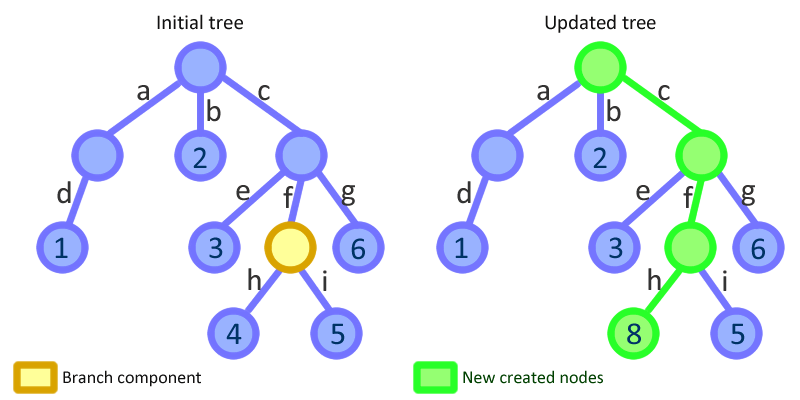
\includegraphics[scale=0.5]{obrazky/immutable_trees}
\par\end{centering}
\caption{Ukázka generování nových imutabilních objektů \cite{immutable_json} \label{fig:immutable_tree}}
\end{figure}

Číslo 4 se v ukázce změnilo na 8, ale více než polovina stromu zůstala zachována. Díky tomu že se jedná o reference, je jejich kopírování velmi rychlé. Nástroj immutable.js, který je dnes asi nejvhodnějším nástrojem pro práci s imutabilními objekty, je úzce svázan s frameworkem React. Síla a rychlost virtuálního DOM, který React používá, je založena na používání imutabilních objektů. Díky nim můžou být operace s virtuálním DOM velmi rychlé. V následujícím grafu je vidět porovnání rychlosti vykreslování webové aplikace, využívající a nevyužívající imutabilní objekty \cite{immutability_graph}. Další zvýšení rychlosti lze docílit použitím PureRenderMixinu v React, který zajistí používání imutabilních struktur i při vykreslování komponent UI \cite{react} \cite{immutablejs_learn}.

\begin{figure}[h]
\begin{centering}
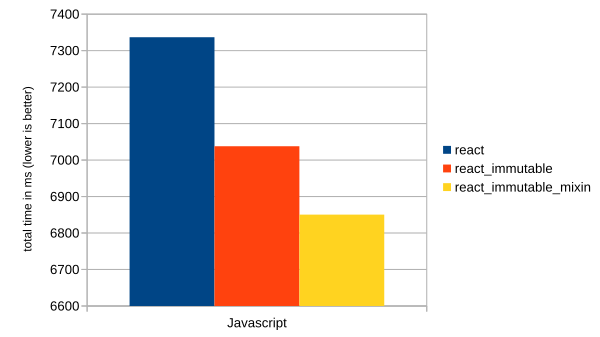
\includegraphics[scale=0.6]{obrazky/immutable}
\par\end{centering}
\caption{Graf rychlostí vykreslování aplikace v React s využitím nebo nevyužitím imutabilních objektů. \cite{immutability_graph} \label{fig:react_immutable}}
\end{figure}
\FloatBarrier 

\section{Vhodné programovací jazyky a nástroje}
Jediným jazykem, který je dnes použitelný na serveru i ve webovém prohlížeči je Javascript. Ten vznikl jako čistě prohlížečový jazyk a díky platformě node.js může nyný sloužit i jako serverový jazyk. Následující kapitola shrnuje nejpoužívanější knihovny a nástroje pro jazyk Javascript, spolu s popisem jejich využití v isomorfních webových aplikacích \cite{isomorhic_book}.

\subsection{node.js}
Není překvapením, že se použití node.js jako serverové části, stává přirozenou volbou nejen pro aplikace závislé na velkém javascriptovém frontendu. Je totiž velmi výhodné používat stejný jazyk pro obě části aplikace. Princip isomorfních aplikací je na používání jediného jazyka založen, použití node.js na straně serveru je tak prakticky jedinou volbou. Tyto aplikace jsou navrženy tak, aby dokázaly ekvivalentně fungovat v prohlížeči i na serveru. Obě části aplikace jsou tak schopny provádět některé operace, například šablony se vykreslují nejdříve na serveru a poté i prohlížeči. Framework React, často používaný pro tvorbu uživatelských rozhraní, funguje bezproblémově na obou prostředích. Serverová část aplikace funguje nejčastěji za pomocí frameworku \textit{express}, který v node.js řeší běžné věci, které programátor očekává od serverového frameworku v některém z běžně používaných jazyků \cite{glover_nodejs} \cite{tilkov_nodejs} \cite{isomorhic_book}.

\subsection{npm}
Balíčkovací systém npm (viz \hyperref[sec:node_js]{2.4}), původně vzniklý pro potřeby serverové platformy node.js, dnes nachází místo i jako systém správy závislostí pro klientskou část aplikace, kde se vždy používal například Bower nebo podobné nástroje \cite{bower}. Npm se stává standardem pro definování závislostí webových aplikací, nalezneme tam téměř všechny běžně používáné javascriptové knihovny. Proto je více než vhodný pro použití v isomorfních aplikacích \cite{npm} \cite{isomorhic_book}.

\subsection{express}
Express je serverový framework pro node.js určený k programování webového serveru v jazyce Javascript. Slouží pro vykreslování HTML, komunikaci s databází, rozhraní pro tvorbu API a další věci, které řeší běžný webový framework v některém ze známých serverových jazyků (PHP, ASP.NET, Python) \cite{express}.

Následující ukázka kódu ilustruje vykreslení HTML šablony pro stránku example.
\begin{lstlisting}[language=Javascript, caption= Ukázkové vykreslení šablony pomocí frameworku express \cite{express}]
var exampleProvider = require('../providers/ExampleProvider'), menuStructure = require('../MenuStructure');

// request handler pro /example
module.exports = function(app) { app.get('/example', function(req, res) {
       var example = exampleProvider.getExample(); 
       var templateData = {
       title: example.title, 
       heading: example.heading, 
       content: example.content, 
       menuStructure: menuStructure
    };
res.render('example', templateData); });
}
\end{lstlisting}

\subsection{Immutable.js}
\label{sec:immutable_js}
Princip imutability dat je popsán spolu s jeho hlavními výhodami v kapitole \hyperref[sec:immutability]{4.3}, imutabilní přístup je pro isomorfní aplikace naprosto zásadní, velmi totiž urychluje práci s daty. Knihovna immutable.js od společnosti Facebook je nejpoužívanějším nástrojem pro práci s imutabilními datovými strukturami \cite{immutablejs}. Byla vytvořena v roce 2014 Lee Byronem kvůli zrychlení DOM manipulací ve frameworku React. Immutable.js nabízí několik persistentních imutabilních struktur \cite{immutablejs}: 

\begin{itemize}
\item List,
\item Stack,
\item Map,
\item OrderedMap,
\item Set,
\item OrderedSet,
\item Record,
\item lazy Seq.
\end{itemize}

Tyto struktury jsou velice rychlé a efektivní, využívají nových možností moderních javascriptových prohlížečových jader jako je \textit{structural sharing}\footnote{Možnost sdílení referencí mezi datovými strukturami.} nebo hashovací datové stromy (hash map tries)\footnote{Vyhledávací datová struktura, která asociuje hašovací klíče s odpovídajícími hodnotami. Hodnota klíče je spočtena z obsahu položky pomocí takzvané hašovací funkce.}. Tyto techniky popisují vysoce optimalizované způsoby ukládání dat. Díky nim je možné minimalizovat nutnost kopírování nebo cachování datových struktur, a tím významně zrychlit manipulace s daty \cite{immutablejs} \cite{immutablejs_learn}.

\subsubsection{List}
List je immutabilní reprezentace klasického javascriptového pole, kde ale každá změna (zpravidla realizována pomocí funkce \textit{push}) vrátí vždy nový imutabilní objekt \cite{immutablejs} \cite{immutablejs_learn}.
\begin{lstlisting}[language=Javascript,caption={Ukázka práce s imutabilním objektem List v immutable.js \cite{immutablejs}}]
var list1 = Immutable.List.of(1, 2);
var list2 = list1.push(3, 4, 5);
\end{lstlisting}

\subsubsection{Stack}
Stack je datová struktura typu FILO\footnote{first in, last out}, která reprezentuje zásobník. Lze si ho představit jako pole, kde první index ukazuje na element, který může být vyjmut pomocí metody \textit{pop()}. Ostatní elementy jsou dostupné pomocí getteru přijímacího index elementu. Modifikace zásobníku, pomocí metod \textit{push()} a \textit{pop()} vrací vždy nový imutabilní zásobník \cite{immutablejs} \cite{immutablejs_learn}.
\begin{lstlisting}[language=Javascript,caption={Ukázka práce s imutabilním objektem Stack v immutable.js \cite{immutablejs}}]
var filo = new Immutable.Stack();
var twoStoreyStack = filo.push( '2nd floor', '1st floor', 'ground floor' );
twoStoreyStack.size // 3
twoStoreyStack.get(1) // "1nd floor"
twoStoreyStack.pop()
twoStoreyStack.size // 2
\end{lstlisting}

\subsubsection{Map}
Imutabilní mapa je klasickou implementací key –> value mapy využívající hashovací funkci. Chová se opět naprosto stejně jako běžná javascriptová mapa, jen každá změna (přidání nebo odebrání objektu) vrátí novou imutabilní mapu \cite{immutablejs} \cite{immutablejs_learn}.
\begin{lstlisting}[language=Javascript,caption={Ukázka práce s imutabilními mapami v immutable.js \cite{immutablejs}.}]
var Immutable = require('immutable');
var map1 = Immutable.Map({a:1, b:2, c:3});
var map2 = map1.set('b', 50); //změna imutabilního objektu, vrátí novou instanci
map1.get('b'); // 2
map2.get('b'); // 50
\end{lstlisting}

\subsubsection{OrderedMap}
OrderedMap je implementace seřazené mapy, vzhledem k imutabilitě ale změna hodnoty na některém z klíčů, nevyvolá opětovné seřazení. To je nutné zajistit ručně pomocí metod \textit{sort()} nebo \textit{sortBy()}, které také, dle očekávání, vrací novou imutabilní mapu \cite{immutablejs} \cite{immutablejs_learn}.
\begin{lstlisting}[language=Javascript,caption={Ukázka práce s imutabilními seřazenými mapami v immutable.js}]
var basket = Immutable.OrderedMap()
                      .set( 'Captain Immutable 1', 495 )
                      .set( 'The Immutable Bat Rises 1', 995 );

console.log( basket.first(), basket.last() ); // 495 995
var basket2 = basket.set( 'Captain Immutable 1', 1095 );
var basket3 = basket2.sortBy( (value, key) -> -value); 
console.log(basket3.first(), basket3.last()); // 995 1095
\end{lstlisting}

\subsubsection{Set}
Imutabilní set je pole unikátních elementů, s obvyklími obslužnými metodami. Přidávání elementů se realizuje pomocí funkce \textit{add()}. Teoreticky tato datová struktura nezajišťuje pořadí uložených elementů. Přidání nebo odebrání elementu vždy vytvoří novou instanci imutabilního setu \cite{immutablejs} \cite{immutablejs_learn}.

\begin{lstlisting}[language=Javascript,caption={Ukázka práce s imutabilním objektem Set v immutable.js \cite{immutablejs}}] 
var s1 = Immutable.Set( [2, 1] );
var s2 = Immutable.Set( [2, 3, 3] );
var s3 = Immutable.Set( [1, 1, 1] );
console.log( s1.count(), s2.count(), s3.count() ); // 2 2 1
\end{lstlisting}

\subsubsection{OrderedSet}
OrderedSet se implementace imutabilního setu s daným pořadím. Elementy jsou řazeny dle data přidání. Jeho použití je totožné s klasickém imutabilním setem, který ale nezaručuje pořadí elementů. Je proto doporučeno používat OrderedSet všude tam, kde je nutné pracovat s elementy ve správném pořadí  \cite{immutablejs} \cite{immutablejs_learn}.

\subsubsection{Record}
Record je imutabilní reprezentací javascriptové třídy s výchozími hodnotami. Je nutné ho instancovat pomocí operátoru \textit{new} jako běžnou třídu. Často slouží jako imutabilní obálka pro datové entity. Dotazování na data funguje pomocí přímého přístupu k vlastnostem objektu, pokud není vlastnost nastavena, vrátí se výchozí hodnota dle definice struktury Record \cite{immutablejs} \cite{immutablejs_learn}.
\begin{lstlisting}[language=Javascript,caption={Ukázka práce s imutabilním objektem Record v immutable.js \cite{immutablejs}}]
var Canvas = Immutable.Record( { width: 1024, height: 768 } );
var myCanvas = new Canvas();
console.log(myCanvas.toJSON()); // Object {width: 1024, height: 768}
console.log(myCanvas.width); // 1024
var myResizedCanvas = new Canvas( {width: 400} );
console.log(myCanvas.toJSON()); // Object {width: 400, height: 768}
console.log(myCanvas.width); // 400
\end{lstlisting}

\subsubsection{lazy Seq}
Knihovna immutable.js také přináší datovou strukturu lazy Seq, česky líná sekvence, která slouží jako imutabilní obálka nad libovolnou kolekcí. Seq umožňuje využívat efektivní funkcionální programování pomocí metod \textit{map} nebo \textit{filter}. Často se používá pro procházení nebo vyhledávání v datových kolekcích. Struktura je lazy, to v programátorské terminoligii znamená, že k jejímu vyhodnocení dojde až při jejím prvním použití, což je zajímavá vlastnost, která také zvyšuje výkon aplikace využívající imutabilní přístup \cite{immutablejs} \cite{immutablejs_learn}.
\begin{lstlisting}[language=Javascript, caption={Ukázka používání lazy Seq v immutable.js \cite{immutablejs_learn}}] 
var seasons = Immutable.Seq( ['spring', 'summer', 'fall', 'winter'] )
                     .filter( season -> season[0]==="s") // pouze začínající na "s"
                     .map(String.toUpperCase);
 
console.log( 'Item at index 0: ', seasons.get( 0 ) ); // SPRING
console.log( 'Item at index 1: ', seasons.get( 1 ) ); // SUMMER
console.log( 'Seasons in an array: ', seasons.toJS() );
\end{lstlisting}

\subsection{React}
\label{sec:react_isomorphic}
Knihovna React, popsaná v kapitole \hyperref[sec:react]{2.8.3} je nejpoužívanější knihovnou pro prezentační vrstvu ve světě isomorfních aplikací. Její úzké zaměření pouze na vykreslování HTML je pro její použití ideální. React také bez problému běží v prostředí node.js, je tedy možné šablony jednoduše vykreslit na serveru a ušetřit tak část práce webovému prohlížeči \cite{react} \cite{react_intro}.
 
Dále následuje popis hlavních částí a implementační detaily knihovny React ve vztahu k programování isomorfních webových aplikací \cite{isomorhic_book}.

\subsubsection{Komponenty}
Základní programovou jednotkou frameworku React je komponenta. Za komponentu lze označit libovolnou část HTML dokumentu, která označuje konkrétní část uživatelského rozhraní webové aplikace. Komponenty slouží pro vykreslování dat. Mohou se libovolně zanořovat, každá komponenta tedy obvykle obsahuje další (vlastněné) komponenty. Vzhledem k tomu, že je v React doporučováno používat syntaxe ES6, lze na každou komponentu nahlížet jako na třídu, přesněji na potomka třídy \textit{React.Component}. Každá komponenta musí implementovat metodu \textit{render()}, ve které je deklarativně definováno související uživatelské rozhraní. To je vždy tvořeno existujícími UI komponentami, které reprezentují buď jednotlivé elementy HTML, například \textit{React.DOM.div}, \textit{React.DOM.input}, nebo jakoukoli komplexnejší programátorem definovanou HTML strukturu. Při vykreslování se komponenty chovají jako funkce, které přebírání HTML vlastnosti (viz níže) a vracejí kompletní HTML kód jednotlivé části webové aplikace \cite{react} \cite{react_intro}.

\subsubsection{Virtuální DOM}
\label{sec:virtual_dom}
DOM (Document Object Model) reprezentuje celou HTML stránku jako hierarchii entit, se kterými lze programově manipulovat pomocí Javascriptu. Možnosti práce s DOM jsou velmi bohaté, lze programově vytvářet, měnit nebo mazat HTML elementy a dostupná je také možnost práce s CSS stylováním. Tyto manipulace jsou nezbytné pro fungování jednostránkových webových aplikací i obecně celé oblasti programování webových aplikací v Javascriptu. DOM jako takový ale nebyl navržen s ohledem na masivní využívání těchto manipulací. Možnost dodatečných úprav stažené webové stránky byla využívána pouze pro jednoduché změny nebo vylepšení. Až moderní javascriptové frameworky přinesly velmi dynamická uživatelská rozhraní, na které není klasický DOM připraven. Jejich obsluha vyžaduje provádět mnoho složitých DOM manipulací, které jsou, při velkém počtu HTML elementů, velmi pomalé. Vezměme si pro představu třeba nějakou známou moderní webovou aplikaci, například Facebook nebo Instagram. Tam každou vteřinu probíhají desítky, ne-li stovky takových DOM manipulací s mnoha různými elementy. Společnost Facebook, jeden z fenoménů dnešní doby, řešila problém s nízkou rychlostí DOM manipulací a navrhla řešení zvané \textit{virtuální DOM}, které je jedním ze základních princpů knihovny React, často zmiňované v této práci. Virtual DOM značí technologii tvorby abstraktního Document Object Modelu spravovaného pomocí Javascriptu uvnitř webového prohlížeče. Framework při každém vykreslování reálného DOM vytvoří také novou verzi toho virtuálního. Nad ním jsou potom realizovány změny. Při následujícím vykreslování je porovnán reálný DOM s tím virtuálním a ta část stromu, která se změnila, se změní i v prohlížeči. Tento postup je znatelně rychlejší než práce přímo s reálným prohlížečovým DOM. Při práci s virtuálním DOM existují především dva problémy, které je třeba řešit \cite{react} \cite{virtualdom}.
\begin{itemize}
\item Kdy reálný DOM překreslovat z toho virtuálního?
\item Jak překreslovat efektivně a rychle?
\end{itemize}

Reálný DOM překreslujeme pokaždé, pokud došlo ke změně dat. A to jen těch, které má zaregistrována některá z aktuálně zobrazených komponent. Pokud se změní data, která nejsou aktuálně zobrazována, je zbytečné provádět překreslení \cite{virtualdom}. Změny v datech lze kontrolovat několika způsoby. Je možné je v pravidelném intervalu procházet a při první nalezené změně vyvolat modifikaci virtuálního a posléze i reálného DOM. Alternativní byť doporučovanou možností je vyvolání změn v DOM na základě nějaké události, například doručení dat ze serveru. Na to je ale nutné myslet při implementraci těchto událostí. Rychlé a efektivní překreslování vyžaduje obecně splňení těchto podmínek \cite{react} \cite{virtualdom}.

\begin{itemize}
\item Efektivní algoritmus pro vyhledávání změn mezi reálným a virtuálním DOM.
\item Realizace zapisovacích operací v dávkách.
\item Efektivní překreslování jen nezbytného části DOM.
\end{itemize}

Všechny zníměné problémy řeší framework React a podobné knihovny, které jsou na konceptu virtuálního Document Object Modelu vystavěny \cite{react} \cite{virtualdom}. Následující diagram dobře ilustruje fungování virtuálního DOM v React.

\begin{figure}[h]
\begin{centering}
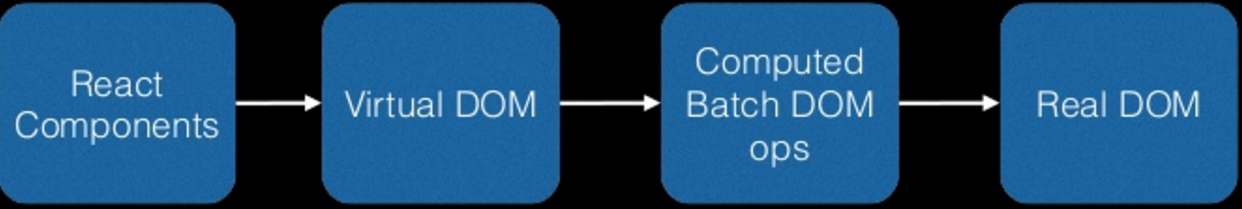
\includegraphics[scale=0.3]{obrazky/virtual_dom}
\par\end{centering}
\caption{Diagram práce virtuálního DOM v React \cite{react} \label{fig:virtual_dom}}
\end{figure}
\FloatBarrier

\subsubsection{JSX}
Jednotlivé komponenty či jejich stromy se ve frameworku React zapisují pomocí speciální syntaxe zvané JSX. Jedná se o rozšíření ECMAScriptu představené spolu s frameworkem React, které přináší novou syntaxi velmi podobnou HTML. Například zápis \textit{<div>text</div>} je frameworkem přeložen na \textit{react.default.createElement('div',null,'text')}, což je sice pochopitelnější konstrukce, ale zase se mnohem hůře čte. JSX se používá nejen pro definici HTML ale především pro řízení zobrazování jednotlivých komponent uživatelského rozhraní \cite{react} \cite{react_book}.

\begin{lstlisting}[language=Javascript,caption={Definice komponenty, která volá jiné komponenty v JSX}]
export default class CommentList extends Component {
render() {
...
  return (
  <div className='comments'>
      <ul>
          <CommentItem key={key} row={key} id={comment.id} editable={editable} comment={comments[0]} {...actions} />
           <CommentItem key={key} row={key} id={comment.id} editable={editable} comment={comments[1]} {...actions} />
            <CommentItem key={key} row={key} id={comment.id} editable={editable} comment={comments[2]} {...actions} />
      </ul>
 	);
 }
}
\end{lstlisting}

Výše uvedená ukázka kódu obsahuje vykreslovací kód komponenty \textit{CommentList} pro zobrazení komentářů v ukázkové webové aplikaci. V ukázce se kombinuje použití klasického HTML s voláním React komponent s parametry, které se nazývají \textit{props} a slouží k přenosu dat z rodičovských komponent. Za zmínku také stojí, že jsou některé HTML atributy v JSX přejmenovány. Jedná se například o atribut class, ktery se zapisuje jako className nebo for, kde se používá htmlFor. Přejmenování bylo nutné, aby nevnikaly kolize s existujícími klíčovými slovy \textit{class} a \textit{for}. Často se stává, že na to vývojář zapomene, proto to framework React dokáže rozpoznat a napoví kde je atribut nesprávně pojmenován \cite{react} \cite{react_book}.

\subsubsection{Props}
\label{sec:react_props}
Framework React rozlišuje data komponent na dva typy. Prvním z nich je stav (state), který tvoří aktuální stav dané komponenty a jen komponenta sama ho může změnit. Druhý typem jsou vlastnosti (properties, zkráceně props), které reprezentují podmnožinu dat webové aplikace a komponenta sama je nemůže nijak měnit. Tyto vlastnosti jsou neměnné a musí být komponentě explicitně předány při jejím zobrazování \cite{react_components} \cite{react_thinking}. Výše uvedená ukázka kódu používá komponentu \textit{CommentItem}, které předává props obsahující: komentář samotný (\textit{comment}), číslo řádku (\textit{row}) a přepínač editace (\textit{editable}). Následující ukázka demonstruje tuto komponentu, která se stará pouze o zobrazení předaných dat (komentářů).

\begin{lstlisting}[language=Javascript,caption={Definice komponenty CommentItem, která zobrazuje komentář}]
export default class CommnetItem extends Component{
render() {
  return(
      <div className='commentItem'>
          <p className='rowNumber'>{row+1}.</p>
          <p className='title' onClick={::this.handleClick}>{comment.text}</p>
          <p className='created'>{moment(modified).fromNow()}</p>
          <p className='outcome'>{comment.author}</p>
    </div>
  );
}
}
\end{lstlisting}

Předávat komponentám lze samozřejmě i funkce či objekty. Props fungují pouze jednosměrně směrem zhora dolů. Komponenta CommentItem nemůže nic předat rodičovské komponentě CommentList. Může však dostat od rodičovské komponenty funkci ve formě callbacku a ten zavolat. Tento jednosměrný postup velmi redukuje komplexnost webových aplikací a tím zjednodušuje správu dat v aplikaci \cite{react} \cite{react_thinking}.

Každá změna props nebo state vždy vyvolá znovuvykreslení komponenty prostřednictvým zavolání funkce \textit{render()} na té komponentě, která zaregistrovala změnu dat. Ta většinou vyvolá překreslení dalších podřízených komponent \cite{react} \cite{react_components}.

\subsubsection{States}
Celá isomorfní webová aplikace nebo všeobecně aplikace bohatě využívající Javascript jsou hluboce založeny na stavech. Nejdříve je nutné si definovat, co je vlastně stav webové aplikace. Zjednoduše řečeno je to vlastně úvodní podoba stránky společně se všemi změnami do okamžiku, kdy tento stav posuzujeme. Zahrnuje DOM elementy a jejich obsah, pořadí, atributy, ale i javascriptové proměnné apod. Způsobů jaké se dnes používají pro reprezentaci stavu webové aplikace je mnoho \cite{zakas_js} \cite{skriptovaci_jazyky}:

\begin{itemize}
\item přidáváním CSS tříd,
\item využití data-* HTML atributů,
\item použití globálních datových struktur Javascriptu ( window.data nebo \$("\#elem").data()).
\end{itemize}

V důsledku těchto postupů jsou data často nepředvídatelně poschovávána na různých místech aplikace. To přináší problémy při implementaci složitějších webových aplikací. Komponenty frameworku React pracují se svým vlastním vnitřním stavem, jehož ukládání je plně v režii frameworku. Tento stav určuje aktuální podobu dané komponenty, vždy dojde-li k jeho změně, zavolá komponenta automaticky metodu \textit{render()} a překlesí se. Změna stavu je většinou spojena například s kliknutím na tlačítko nebo se změnou souvisejícího formulářového prvku. Původní koncept frameworku React počítal s tím, že pouze komponenta sama může provádět změny svého stavu. Striktně lokální povaha tohoto stavu ale komplikuje možnosti ovládání dané komponenty, proto je dnes doporučované předávat komponentě celý její stav zvenčí pomocí parametru. Veškerá data, která komponenta potřebuje, předáváme jako její \textit{props} pomocí nadřazené komponenty. Hovoříme potom o takzvaných \uv{stateless (bezstavových) komponentách}. Všechny lokální stavy všech komponent by měly být uloženy na jednom místě. Tím místem je podle principu \uv{jediného zdroje pravdy} (single source of truth), úložiště \textit{store} z architektury Flux (viz. \hyperref[sec:flux]{4.4.6}) \cite{react} \cite{react_book}  \cite{flux} \cite{react_thinking}.

Store obsahuje všechna data aplikace a ostatní komponenty na tato data nahlíží a reagují na ně. Když se data změní, komponenty se překreslí. Žádná komponenta nikdy nezjišťuje stav jiné komponenty, vždy se dívá pouze do store. Data vyjadřují aktuální stav aplikace a stejná data musí vždy aplikaci uvést do stejného stavu. Tomuto principu se říká \uv{předvídatelný stav} (predictable state). Z takového přístupu plyne mnoho výhod. Například ladění je velmi snadné, protože všechny změny prochází jediným místem, do kterého můžeme nahlédnout. Také můžeme jednoduše implementovat funkci undo – vracení akcí zpět \cite{react_book} \cite{flux} \cite{react_thinking}.

\subsubsection{Vykreslování HTML}
Webová aplikace využívající React je vždy celá překreslena při každé změně stavu. Vývojáři tohoto frameworku zastávájí názor, že je jazyk Javascript již dostatečně výkonný, aby bylo rychlé překreslování možné. Tím je odstraněna potřeba data někde předem výpočítávat a dočasně ukládat. Veškeré výpočty by měli být prováděny až v metodě \textit{render()} každé React komponenty, aby se předešlo problémům s konzistencí dat. Vykreslování HTML probíhá pomocí volání zmíněné metody \textit{render()} od kořenové aplikační komponenty (často zvané Root nebo WebApplication) rekurzivně přes celý strom komponent. Překreslení některého z podstromů je možné pro zlepšení výkonu omezit implementováním metody \textit{shouldComponentUpdate()}, která provede porovnání aktuálního a nového stavu komponenty a vrátí pravdivostní hodnotu, zda je nutné daný podstrom překreslit nebo ne \cite{react} \cite{react_components} \cite{react_book}.

\subsubsection{Delegování událostí}
Další důležitou vlastností React je možnost delegování událostí, které zefektivňuje práci s DOM a vylepšuje práci s pamětí. Ke každé komponentě je možné přiřadit nějakou obsluhu událostí, ve skutečnosti však existuje jeden jediný posluchač, připojený na nejvyšší úrovni Document Object Modelu, jež obaluje veškeré události prohlížeče a předáva je do virtuálního DOM. To umožňuje předat obsluhu události správné komponentě aniž by docházelo ke ztrátě výkonu. Správa připojených posluchačů probíhá na interní bázi frameworku, není tedy nutné pracovat s reálným DOM. Automatická správa posluchačů je u moderního webového frameworku nezbytností \cite{react} \cite{react_components}. Podle Zakas je obrovský počet, často již nepoužívaných posluchačů navěšených na DOM elementy, jedním z hlavních zdrojů problémů s výkonem a paměťovou náročností moderních javascriptových webových aplikací \cite{zakas_js}.

\subsubsection{React router}
Velmi podstatnou částí každé webové aplikace je router, který zpracovává HTTP požadavky a podle URL a vstupních dat iniciuje příslušné části aplikace. U jednostránkových aplikací, kam isomorfní aplikace spadají, není možné použít klasický serverový MVC přístup, protože routování probíhá uvnitř webového prohlížeče. Je nutné použít nějaký router pro Javascript. Knihovna React nabízí nástroj \textit{React-router}, který řídí tok dat v aplikaci, mění aktuální URL nebo zajištuje správné fungování historie i tlačítka zpět. Router také řeší zpracování a předávání parametrů obslužným metodám. Jednotlivé definice vstupních částí aplikace spolu s připojenými React komponentami se nazývají routovací pravidla a jsou zapisována pomocí syntaxe JSX \cite{react} \cite{react_router}.

\begin{lstlisting}[language=Javascript,caption={Ukázka definice routování pomocí React-router \cite{react_router}}]
   <Router history = {browserHistory}>
      <Route path = "/" component = {App}>
         <IndexRoute component = {Home} />
         <Route path = "home" component = {Home} /> // na /home iniciuj komponentu Home
         <Route path = "about" component = {About} />
         <Route path = "contact" component = {Contact} />
      </Route>
   </Router>
\end{lstlisting}

Při použití isomorfního přístupu je většinou nutné používat jeden router na straně serveru a druhý na straně webového prohlížeče. Moderní isomorfní devstacky ale dokážou propagovat jednou definovaná routovací pravidla do obou routerů \cite{react_book} \cite{react_router}.

\subsection{Flux}
\label{sec:flux}
Společnost Facebook také navrhla architekturu správy dat známou jako Flux, která řeší mnohé problémy běžných MVC frameworků se správou dat. Jedná se o návrhový vzor, který se aplikuje při návrhu jednosměrného toku dat v aplikaci. Vychází z předpokladu, že výsledné UI je reprezentovatelné pomocí dat, které do něj tečou z úložišť (Store). Interakce uživatelů jsou reprezentovány pomocí akcí (Actions). Akce zpracovává dispečer (Dispatcher), který následně notifikuje o změnách jednotlivá úložiště, ty změnu provedou a reflektují ji do UI komponent které je poslouchají \cite{react_book} \cite{flux}.

\vspace{3mm}
\noindent Architektura flux má několik základních pravidel \cite{react_book} \cite{flux}.

\begin{itemize}
\item Všechna data v úložištích mohou být měněny pouze skrz akce.
\item Všechny akce vstupují do úložiště skrze jediný bod vstupu 
\item Není možné provést novou akci dokud ta aktuální neskončí. To také znamená, že všechny úložiště jsou zaktualizovány najednou, a vždy nechají aplikaci v konzistentním stavu (princip transakce).
\item Data uvnitř úložišť jsou přístupná z vnějšku pouze skrz read-only veřejné API.
\end{itemize}

Důsledkem jejich dodržování je to, že v jakýkoliv okamžik je velice jednoduché si udělat představu o tom, co se uvnitř úložišť děje \cite{react_book}. Následující obrázek dobře ilustruje fungování celé architektury.

\begin{figure}[h]
\begin{centering}
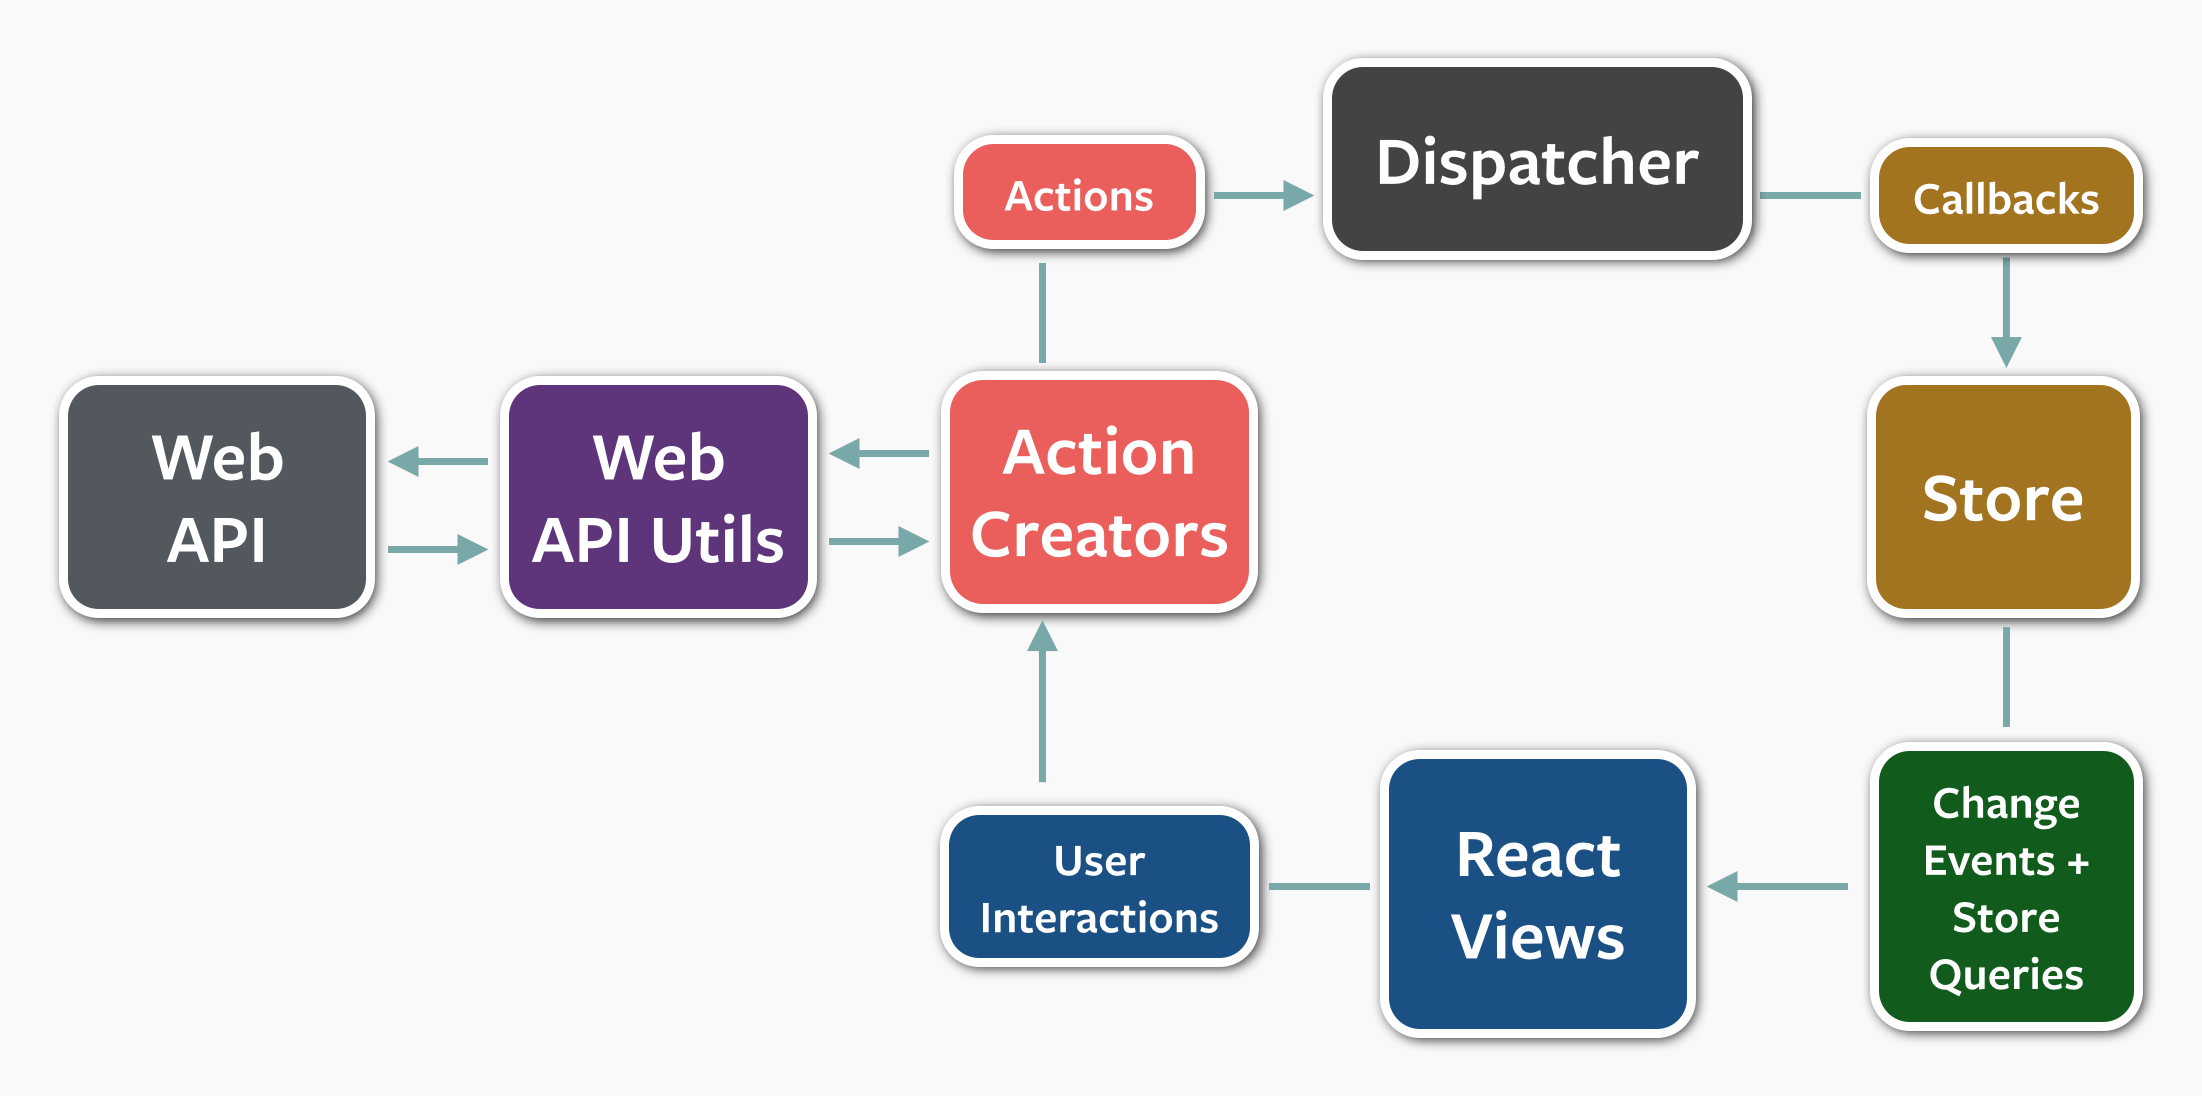
\includegraphics[scale=0.3]{obrazky/flux_architecture}
\par\end{centering}
\caption{Diagram architektury Flux \cite{flux} \label{fig:flug_architecture}}
\end{figure}
\FloatBarrier

I když Flux přináší mnoho výhod a řeší některé aktuální problémy javascriptových aplikací, má také mnoho nevýhod. Především je to pomalá křivka učení, nové implementační koncepty a složitý kód. Flux jako takový je ale pouze návrhovým vzorem, který nelze stáhnout a používat. Je nutné použít některou z jeho implementací. Mezi neznámější z nich patří \textit{Redux}, \textit{Delorean}, \textit{Lux}, \textit{Reflux} nebo \textit{OmniscientJS} \cite{flux_comparison}. První jmenovaný je v současné době doporučovaný a používá ho i ukázková aplikace v této práci. Redux je predikovatelný stavový kontejner pro javascriptové aplikace. Pomáhá psát konzistentní, dobře testovatelné aplikace, které můžou běžet na všech dostupných javascriptových platformách. Vývojářům také přináší nové možnosti jako je živá editace kódu nebo time-traveling debugger\footnote{Debugování, při kterém lze přepínat mezi předchozími aplikačními stavy a tím se fakticky \uv{vracet v čase}.}. Redux pracuje dle principu Flux, ale dispatcher nahrazuje takzvaným \textit{reducerem}. Jedná se o obyčejnou funkci, která je vložena do úložiště, aby bezpečně modifikovala data dle proběhlých akcí. V momentě doručení akce do úložiště, je zavolán reducer kterému je předán současný stav aplikace a provedené akce. Uvnitř reduceru je kód, který podle identifikace akce provede požadovanou změnu dat a vrátí jejich novou podobu – nový aplikační stav \cite{flux} \cite{redux}.

\subsection{Task runnery}
\label{sec:task_runners}
Svět programování webových aplikací v Javascriptu se neobejde bez používání mnoha knihoven. Je tedy zapotřebí někdo, kdo pomůže zautomatizovat proces vývoje například tím, že bude kontrolovat syntaxi CSS a Javascript souborů, kompilovat soubory z CSS preprocesorů (LESS, SASS, Stylus) do CSS, překompilovávat CoffeeScript do čistého Javascrptu, spojovat soubory, minifikovat, nasazovat do různých prostředí nebo generovat dokumentaci podle JSDoc. Tento proces se také nazývá buildování webové aplikace. Pro tento účel se používají knihovny zvané task runnery, většinou implementovány v Javascriptu pomocí node.js. Pro jejich docenění je nejdříve potřeba pojmenovat zásadní problém, kterému vývojáři webových aplikací čelí. Webové aplikace jsou distribuovány pomocí pomalého a nespolehlivého protokolu HTTP do vzdáleného prohlížeče. Tam se musí celá webové stránka zpracovat, spustit a něco vykonat. Výsledná velikost webové aplikace je tedy značně limitována, protože příliš dlouhé načítání je dnes zásadní problém. Aby vše fungovalo svižně, je třeba co nejvíce omezit množství nezbytných HTTP dotazů a co nejvíce minimalizovat jejich velikost. Jinými slovy je nutné pečlivě zvážit, co a kdy posílat do webového prohlížeče, v jakém pořadí a po jakých částech. Pro většinu webových aplikací stačí celou aplikaci spojit do jednoho souboru, pojmenovaného například \textit{app.js}. Tento způsob je často využíván v task runnerech Grunt a Gulp. Ovšem tento soubor může mít časem značnou velikost, proto je také možné sestavit (build) webovou aplikaci jako více ucelených částí dle jejich účelu, a ty poté dodávat do jednotlivých webových stránek. To doporučuje jiný task runner \textit{Webpack} \cite{webpack}. Tyto tři dnes nejpoužívanější task runnery, jsou popsány na následujících řádcích. Existuje více takových nástrojů, tři zmíněné jsou však současným mainstreamem pro vývoj v Javascriptu \cite{task_runners} \cite{zdrojak_gulp}.

\vspace{0,3cm}
\noindent Všechny tři zmiňované nástroje mají několik společných vlastností \cite{zdrojak_gulp}.
\begin{itemize}
\item Jsou napsány v Javasciptu – pro svůj běh vyžadují nodejs.
\item Ovládají se prostřednictvím příkazové řádky.
\item Mají velmi aktivní komunitu 
\item Každý trochu jiným způsobem řeší identickou oblast vývojářského života.
\item Opensource licence MIT
\end{itemize}

\subsubsection{Grunt}
Grunt.js byl jedním z prvních task runnerů a rychle si ho oblíbila celá Javascriptová komunita. Jeho autorem je Ben Alman a vznikl v roce 2012 \cite{grunt_intro}. Tento nástroj slouží pro automatizaci opakovaných úloh při vývoji javacriptové aplikace. Grunt upřednostňuje psaní konfigurace před psaním kódu \cite{grunt}. 

\pagebreak
\noindent Krátká ukázka toho, jak vypadá soubor Gruntfile.js \cite{grunt} \cite{zdrojak_gulp}:
\begin{lstlisting}[language=Javascript,caption={Ukázka syntaxe souboru Gruntfile.js}]
module.exports = function(grunt) {
  grunt.initConfig({
    uglify: {
    something: {
     files: {
       'dest/output.min.js': ['src/input1.js', 'src/input2.js']
     }
    }
   }
  });
  // načteme externí modul
  grunt.loadNpmTasks('grunt-contrib-uglify');
  // přidáme úlohu
 grunt.registerTask('stable-build', ['...', '...']);
};
\end{lstlisting}
\noindent Některé nevýhody task runneru Grunt \cite{zdrojak_gulp}:
\begin{itemize}
\item Konfigurace místo psaní Javascript kódu, konfigurační soubory Gruntfile jsou zpravidla delší.
\item Velké množství parametrů pro konfiguraci jednotlivých pluginů.
\item Je pomalejší při zpracování většího počtu souboru (příliš mnoho I/O operací).
\item Konkurenční zpracování úloh se řeší složitěji nebo prostřednictvím pluginu.
\end{itemize}

\subsubsection{Gulp}
Grunt klade důraz na konfigurovatelnost, takže je vhodnější pro uživatele, kteří chtějí spíše konfigurovat, než psát vlastní kód. Tím vzniká u větších projektů často obrovský a nepřehledný konfigurační soubor Gruntfile. Nástroj Gulp jde cestou psaní vlastního kódu, díky čemu je konfigurace kratší a srozumitelnější. Gulp vznikal v polovině roku 2013 pod hlavičkou společnosti Fractal. Jeho autorem je Eric Schoffstall. Jeho cílem bylo vše zjednodušit a zrychlit. Gulp masivně využívá node.js streamy, díky čemuž je většinou rychlejší než konkureční nástroj Grunt. Data se mezi jednotlivými úlohami předávají prostřednictvím pipeline\footnote{Zřetězené zpracovávání dat ve kterém výstup první části je vstupem té druhé a tak dále.}. Redukuje se tím počet I/O diskových operací a úlohy se dají snadno řetězit \cite{gulp} \cite{gulp_web} \cite{zdrojak_gulp}.

\pagebreak
\vspace{0.3cm}
\noindent Krátký příklad, jak může vypadat Gulpfile.js \cite{zdrojak_gulp}:
\begin{lstlisting}[language=Javascript,caption={Ukázka syntaxe souboru Gulpfile.js}]
var gulp = require('gulp'),
var uglify = require('gulp-uglify');
gulp.task('compress', function() {
  gulp.src(['lib/*.js'])
    .pipe(uglify())
    .pipe(gulp.dest('dist'))
});
gulp.task('default', function() {
  gulp.run('compress');
});
\end{lstlisting}

Zde je dobře viditelná základní myšlenka task runneru Gulp: Stručný a přehledný kód je lepší než složitá konfigurace \cite{gulp} \cite{zdrojak_gulp}.

\vspace{0,3cm}
\noindent Některé nevýhody task runneru Gulp \cite{zdrojak_gulp}.
\begin{itemize}
\item Masivní používání streamů může být pro začátečníka matoucí. 
\item Složitý postup pří řešení lineární závislostí jednotlivých úloh.
\item Obvykle minimální možnosti konfigurace pluginu.
\item Menší množství pluginů.
\end{itemize}

\subsubsection{Webpack}
\label{sec:webpack}
Nový nástroj pro automatizaci vývoje, přinášející opět nové koncepty se jmenuje Webpack. Ten sice vyšel už v roce 2012, ale začíná se masivně používat až v posledních zhruba dvou letech. Jeho autorem je Tobias Koppers. Webpack se oficiálně označuje jako \textit{module bundler}, není tedy typickým task runnerem, i když dokáže Gulp nebo Grunt často plně nahradit. Správu závislostí ale řeší zcela jiným způsobem, jediné co vývojář webové aplikace musí udělat, je vždy explicitně uvádět závislosti. Webpack pak potom celou aplikace projde a vytvoří kompletní graf závislostí. Na základě něj potom sestaví jeden nebo více výstupních souborů, zvaných \textit{bundles} \cite{webpack} \cite{webpack_book}.

\begin{figure}[h]
\begin{centering}
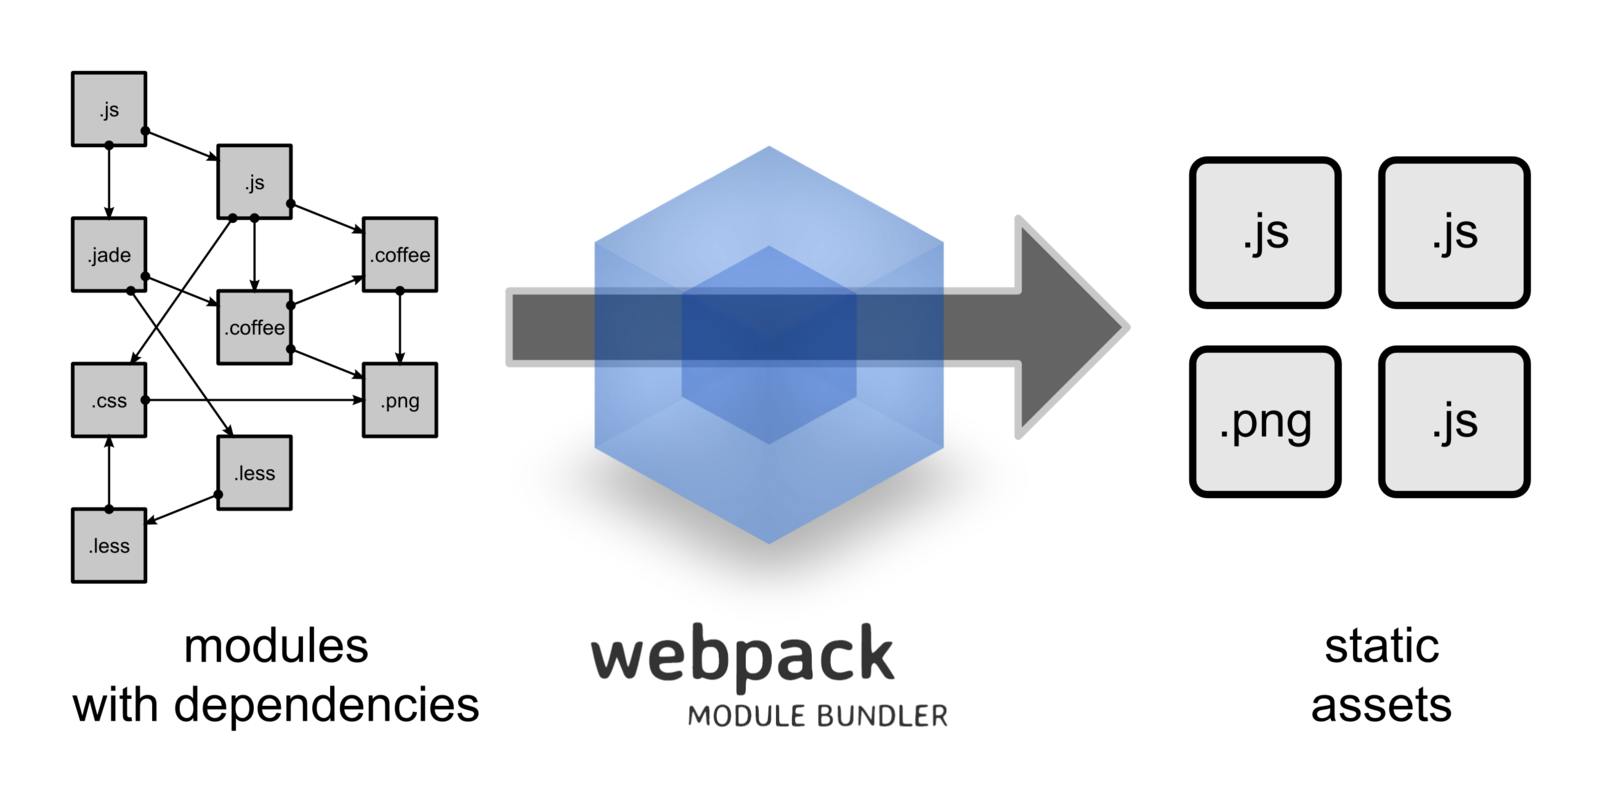
\includegraphics[scale=0.7]{obrazky/webpack}
\par\end{centering}
\caption{Diagram ilustrující způsob fungování module bundleru Webpack \cite{webpack_book}. \label{fig:webpack}}
\end{figure}
\FloatBarrier

Je nutné nakonfigurovat vstupní bod aplikace, ze kterého je zahájeno prohledávání a definovat jednotlivé loadery. Loader v kontextu Webpacku znamená program, který umí číst a zpracovávat nějaký formát. Myšlenka webpacku totiž spočívá v tom, že je možné explicitně uvádět (importovat) Javascript, CSS, obrázky, fonty a vlastně úplně cokoliv co daná stránka nebo komponenta potřebuje. Stačí použít správný loader pro všechny formáty. Výstup pak bude 100\% optimální. Každá část aplikace dostane jen tolik zdrojů, kolik skutečně potřebuje a nic zbytečně navíc. Mezi často používané loadery patří například SASS-loader nebo Babel-loader. Webpack také řeší spuštění a správu vlastního vývojového webového serveru. Tento server si hlídá všechny podmíněné soubory, tedy soubory, které jsou zdrojové pro výsledný bundle a pokud se některý z nich změní, hned vygeneruje nový bundle \cite{webpack} \cite{webpack_book}.

Jednou z nejzajímavějších vlastností Webpacku je Hot Module Replacement, česky výměna modulů za běhu. Díky tomu je možné vyměňovat části aplikace bez nutnosti jejího restartu. Webpack automaticky do každého vygenerovaného bundle přidá krátký kód, který běží uvnitř spuštěné aplikace. Když se něco v aplikaci změní (tedy vznikne nový bundle), přidáný kód nahlásí změnu daného modulu webpacku. Ten se potom pokusí nahradit pouze změněný modul, pokud to není možné, nahradí rodičovský modul. To se opakuje dokud není nahrazení provedeno nebo HMR dosáhnul vstupního bodu aplikace a nahrazení za běhu tak není možné provést. Potom dojde k chybě a je nutné provést restart celé aplikace. Webpack je velký a mocný nástroj, který je zároveň i extrémně modulární díky obrovskému množství loaderů a pluginů. Není však úplně snadné ho nastavit \cite{webpack} \cite{webpack_book}. Následuje ukázka jeho základní konfigurace, reálná konfigurace bývá násobně složitější. Hlavní částí je definice \textit{loaderů}, které zpracovávají jednotlivé soubory. 

\pagebreak
\begin{lstlisting}[language=Javascript,caption={Ukázka konfigurace module bundleru Webpack}]
module.exports = {
  entry: './main.js', // definice vstupního bodu aplikace
  output: {
    filename: 'bundle.js' // výstupní soubory
  },
  module: { 
    loaders: [ // jednotlivé loadery pro dané jazyky
      { test: /\.coffee$/, loader: 'coffee-loader' }, // loader pro coffeescript
      {
        test: /\.js$/,
        loader: 'babel-loader', // loader pro Babel
        query: { presets: ['es2015', 'react']} // Babel presety
      }
    ]
  }
};
\end{lstlisting}

\section{Ukládání dat}
Jako datová úložiště používají moderní javascriptové webové aplikace většinou NoSQL databáze. Tyto databáze nemají definovaná schémata, strukturu dat lze vynutit pouze validačními funkcemi. Ukládání dat se většinou realizuje pomocí formátu JSON, hovoříme potom o \textit{JSON dokumentu}. JSON je textový formát vycházející z podmnožiny syntaxe objektových literálů Javascriptu, je tvořen dvojicemi klíč-hodnota, kde hodnotou může být další taková dvojice, proto je libovolně strukturovatelný \cite{json}. O dokumentu hovoříme tehdy, obsahuje-li datový model  většinu souvisejících dat přímo v sobě, ne ve formě odkazů na další entity, analogie s běžným papírovým dokumentem. Tyto dokumenty často kopírují datové entity v Javascriptu \cite{ja}. Mezi často používané NoSQL databáze například MongoDB, v posledních letech je také populární realtime databáze RethinkDB, která je díky své rychlosti a dobré škálovatelnosti velmi vhodná pro isomorfní webové aplikace \cite{rethinkdb}. Je také použita v ukázkové aplikaci, popsané v praktické části práce.

\section{Vybrané devstacky}
\label{sec:devstacks}
Každé vývojové prostředí javascriptového projektu se obecně skládá z množiny spolupracujících knihoven, běžících pomocí node.js, jejichž vzájemnou interakci může být složité nakonfigurovat. Připravený soubor knihoven nebo frameworků, spolu s nástroji pro usnadnění práce vývojáře, se nazývá \textit{devstack}. Ten řeší komunikaci mezi jednotlivými částmi aplikace, sestavování (build) aplikace, řízení vývojového webového serveru nebo spouštění testů. Devstacky pro isomorfní webové aplikace řeší především níže uvedené požadavky. V závorce jsou vždy nejznámější používané javascriptové knihovny, které tyto oblasti pomáhají řešit \cite{isomorphic_pimentel}.

\begin{itemize}
\item Zpracovávání HTTP requestů (Superagent, Axios).
\item Routování URL (Director, react-router).
\item Vykreslování HTML (React, Handlebars).
\item Podporu modularizace (FormatJS, Browserify, Webpack).
\item Nástroje pro sestavení aplikace, task runnery (Webpack, Grunt, gulp.js).
\item JS transpilery (Babel, CoffeeScript, Purescript).
\item CSS procesory (Sass, Less).
\item Polyfilly pro podporu starších prohlížečů.
\item Minifikační, obfuskační nástroje (uglify.js, JSMin, CSSMin).
\item Knihovny pro isomorfní přístup (babelify, browserify, isomorphic-tools).
\end{itemize}

Následující kapitola se zabývá představením pěti vybraných devstacků vhodných pro vývoj isomorfních webových aplikací v jazyce Javascript.

\subsection{Este.js}
Prvním vybraným devstackem je Este.js, které vyšlo v roce 2013. Jedná se o isomorfní devstack od českého vývojáře Daniela Steigerwalda. Este.js samo sebe popisuje jako: \uv{nejbohatší starter kit\footnote{Připravené vývojové prostředí s příklady vhodnými pro seznámení se s danou technologií.} pro vývoj isomorfních funkcionálních webových aplikací} a jeho motto je: \textit{zapomeňte na frameworky, učte se návrhové vzory}. Což je do značné míry příznačné, protože knihoven existuje mnoho, zatímco návrhových vzorů méně a jejich znalost je pro vývoj webových aplikací důležitější. Este používá Facebook architekturu uživatelského rozhraní, Redux pro správu aplikačních stavů a programuje se v moderním ES6 Javascriptu. Zajímavostí může být použití statického type checkeru, který pomáhá objevovat nečekané chyby pomocí vyhodnocování datových typů v Javascriptu. Este neřeší otázku výběru vhodné databáze, autor však doporučuje použití Firebase. Devstack je dostupný na serveru GitHub \cite{este} \cite{isomorphic_pimentel}.

\vspace{0,3cm}
\noindent \textbf{Použité technologie}:
\begin{itemize}
\item \textbf{React} – komponenty UI.
\item \textbf{Redux} – implementace Flux architektury pro správu dat.
\item \textbf{ExpressJS} – serverová část.
\item \textbf{BabelJS} – transpiler ES6 Javascriptu.
\item \textbf{FlowType} – static type checker.
\item \textbf{react-router} – routování uživatelských požadavků.
\item \textbf{Jest} – unit testování.
\end{itemize}

\begin{table}[h]
\centering
	\caption{Výhody a nevýhody isomorfního devstacku Este.js \cite{isomorphic_pimentel}}
	\begin{tabular}{ |C{5cm}|C{5cm}| }
	\hline
	Výhody & Nevýhody \\ \hline
	UI architektura Facebooku & Málo kvalitní dokumentace a příkladů \\ \hline
	Kompletní podpora server-side renderingu & Časté změny implementace\\ \hline
	Používání ES6 Javascriptu & Známější jen v českém prostředí.\\ \hline
	Imutabilní globální stav aplikace & Větší křivka učení\\ \hline
	Skvělý výkon & \\ \hline
    \end{tabular}
	\label{tab:proscons_este}
\end{table}
\FloatBarrier

\subsection{IMA.js}
IMA.js je další český devstack, od společnosti Seznam, která ho nejdříve vytvořila pro interní účely, aby ho potom uvolnila jako open source na serveru GitHub. Je také postaven na zobrazovací vrstvě v React a backendu nad node.js pomocí Expressu. V současnosti ho používá například herní portál hry.cz. IMA.js neřeší otázku persistence dat, výběr databáze a implementace komunikace s ní je tedy čistě na programátorovi \cite{ima}.

\pagebreak
\vspace{3mm}
\noindent \textbf{Použité technologie}:
\begin{itemize}
\item \textbf{React} – komponenty UI.
\item \textbf{ExpressJS} – serverová část.
\item \textbf{BabelJS} – transpiler ES6 Javascriptu.
\item \textbf{Superagent} – framework pro komunikaci s API.
\item \textbf{Jasmine} – unit testování.
\item \textbf{Winston} – logování.
\end{itemize}

\begin{table}[h]
\centering
	\caption{Výhody a nevýhody isomorfního devstacku IMA.js \cite{ima}}
	\begin{tabular}{ |C{5cm}|C{5cm}| }
	\hline
	Výhody & Nevýhody \\ \hline
	Kvalitní dokumentace & Téměř nulová komunita \\ \hline
	Kompletní podpora server-side renderingu & Složitější konfigurace \\ \hline
	Využití nejmodernějších knihoven & Vytvořeno pro interní využití jedné firmy \\ \hline
	Jednoduché testování & \\ \hline
    \end{tabular}
	\label{tab:proscons_ima}
\end{table}
\FloatBarrier

\subsection{Meteor}
Jedním z nejpopulárnějších devstakců je také Metero, ten byl představen v prosinci roku 2011 týmem vývojářů z technologického akcelerátoru Y-Combinator. Jedná se o sadu nástrojů, které vývojářům pomáhají s vývojem webových nebo mobilních aplikací. Meteor řeší frontend, backend, balíčkování i nasazování, jeho filozofie zní \textit{Javascript everythere}. Společnost, která vznikla pro zastřešení jeho dalšího vývoje, dostala v roce 2012 investici 11,2 milionu dolarů od několika amerických investorských skupin. Je to první javascriptový nástroj, který získal investici v podobné výši. Díky ní byl zahájen bouřlivý vývoj Meteoru, který vyústil v implementaci vlastního testovacího, šablonovacího i balíčkovacího systému. Právě používání vlastních řešení a snaha o přílišnou komplexnost jsou v Meteoru často terčem kritiky. Synchronizace mezi klientem a serverem řeší Meteor zcela automaticky pomocí protokolu Websocket. Další zajímavostí je provádění databázových operací na klientu i na serveru. Meteor obsahuje \textit{minimongo}, což je implementace databáze MongoDB v Javascriptu pro použití v prohlížeči. Data se tak ukládají ihned lokálně a poté jsou asynchronně replikována do hlavní MongoDB databáze \cite{isomorphic_pimentel} \cite{meteor} \cite{meteor_web}.

\vspace{0,3cm}
\noindent\textbf{Použité technologie}:
\begin{itemize}
\item \textbf{Blaze} – reaktivní UI komponenty.
\item \textbf{DDP} – real-time komunikační protokol pro Websocket.
\item \textbf{Minimongo} – jednoduchá databáze pro webový prohlížeč replikovaná do hlavní databáze.
\item \textbf{MongoDB} – jediná kompatibilní hlavní databáze.
\item \textbf{Velocity} – testovací framework.
\end{itemize}

\begin{table}[h]
\centering
	\caption{Výhody a nevýhody isomorfního devstacku Meteor \cite{isomorphic_pimentel}}
	\begin{tabular}{ |C{5cm}|C{5cm}| }
	\hline
	Výhody & Nevýhody \\ \hline
	Velmi jednoduché na použití, mnoho kvalitní dokumentace a příkladů. & Funguje pouze s MongoDB (na Redis implementaci se pracuje). \\ \hline
   Připravený autentizační nástroj & Pouze částečná podpora server-side renderingu \\ \hline
   Možnost generování mobilních aplikaci & Používání vlastního šablonovacího jazyka \\ \hline
   Velká uživatelská základna & Občas dogmatický přístup autorů \\ \hline
    \end{tabular}
	\label{tab:proscons_meteor}
\end{table}

\subsection{DerbyJS}
DerbyJS vzniklo v roce 2011 jako jeden z prvních isomorfních devstacků pro node.js. Dnes je asi největším konkurentem platformy Meteor. DerbyJS používá vlastní šablonovací jazyk, který svojí syntaxí vychází z Handlebars. Pro manipulaci s daty se používá speciální engine Racer, který zajišťuje propagaci změn v reálném čase nebo řeší konflikty mezi daty. Umí také pracovat v režimu offline, po opětovném připojení data automaticky odešle na server. K tomu se využívá vlastní frontend databázi LiveDB, pro hlavní databázi je doporučováno MongoDB, lze ale využít i jiných databází. Také devstack DerbyJS je dostupný na serveru GitHub \cite{isomorphic_pimentel}  \cite{derbyjs}.

\pagebreak
\vspace{3mm}
\noindent\textbf{Použité technologie}:
\begin{itemize}
\item \textbf{ExpressJS} – serverová část.
\item \textbf{RacerJS} – framework pro synchronizaci modelů.
\item \textbf{ShareJS} – zajišťuje uživatelské interakce v reálném čase.
\item \textbf{LiveDB} – frontend databáze.
\item \textbf{MongoDB} – hlavní databáze (podporuje i jiné databáze při použití ORM nástroje jako například SequelizeJS).
\end{itemize}

\begin{table}[h]
\centering
	\caption{Výhody a nevýhody isomorfního devstacku DerbyJS \cite{isomorphic_pimentel}}
	\begin{tabular}{ |C{5cm}|C{5cm}| }
	\hline
	Výhody & Nevýhody \\ \hline
	Kompletní podpora server-side renderingu & Zatím v rané fázi vývoje \\ \hline
   Automatické řešení konfliktů uživatelských stavů & Velmi málo dostupné dokumentace.\\ \hline
	Intuitivní souborová struktura projektů & \\ \hline
    \end{tabular}
	\label{tab:proscons_este}
\end{table}
\FloatBarrier

\subsection{Rendr}
Posledním vybraným isomorfním devstackem je Rendr, který vznikl v komunitě kolem frameworku Backbone.js. Rendr obecně je pouze nástroj pro provozování Backbone.js aplikace na serveru. 

Umožňuje spojit server-side rendering a datové API s tradiční jednostránkovou aplikací napsanou ve zmíněném frameworku. MVC framework Backbone.js je často používaným řešením, existuje pro něj mnoho knihoven a kvalitní dokumentace. Rendr pouze integruje mnohé z nich a umožňuje provozovat klasickou SPA webovou aplikaci dle isomorfncího přístupu \cite{isomorphic_pimentel} \cite{rendrjs}.

\vspace{0,3cm}
\noindent\textbf{Použité technologie}:
\begin{itemize}
\item \textbf{BackboneJS} – frontend MVC framework.
\item \textbf{HandlebarsJS} – šablonovací systém.
\item \textbf{ExpressJS} – serverová část.
\item \textbf{MongoDB} – hlavní databáze.
\end{itemize}

\pagebreak
~
\begin{table}[h]
\centering
	\caption{Výhody a nevýhody isomorfního devstacku Rendr \cite{isomorphic_pimentel}}
	\begin{tabular}{ |C{5cm}|C{5cm}| }
	\hline
	Výhody & Nevýhody \\ \hline
	Podporuje většinu nástrojů z komunity kolem Backbone.js & Starší dokumentace \\ \hline
	Plná podpora server-side renderingu & Neřeší všechny oblasti vývoje webových aplikací \\ \hline
    Jednoduchá konfigurace & \\ \hline
    \end{tabular}
	\label{tab:proscons_rendr}
\end{table}

\chapter{Ukázková webová aplikace}
V následující kapitole je představena ukázková webové aplikace, vyvinutá dle isomorfního přístupu, popsáného výše. Serverová i klientská část aplikace je tedy napsána v jazyce Javascipt. Tento přístup sjednocuje použitý jazyk a knihovny pro obě části aplikace a tím zjednodušuje a sbližuje implementaci celého systému moderní webové aplikace. Datová komunikace webového prohlížeče se serverem probíhá pomocí Websocketu. Server zasílá klientovi data ve formátu JSON (Javascript Object Notation \cite{json})). Ukázková webová aplikace představuje jednoduchou návštěvní knihu se základní funkcionalitou. Vytvořenou aplikaci můžeme zařadit mezi takzvané Rich Internet Applications \cite{ria}, tedy webové aplikace jejichž uživatelské prostředí se snaží uživateli poskytnout prostředky, které zná z běžných desktopových aplikací. Na rozdíl od tradičních webových aplikací není uživatelské prostředí tvořeno pouze základními prostředky jazyka HTML, ale hojně využivá javascriptové komponenty, implementované ve frameworku \textit{React} \cite{react}, který je zodpovědný za návrh a obsluhu interaktivního uživatelského rozhraní. Návod ke spuštění a instalaci ukázkové aplikace lze nalézt v přílohách této práce.

\vspace{3mm}
\begin{figure}[h]
\begin{centering}
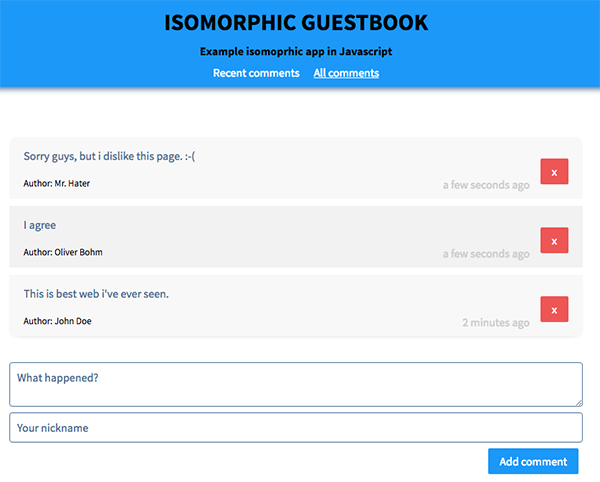
\includegraphics[scale=0.45]{obrazky/example_app}
\par\end{centering}
\caption{Ukázka vytvořené isomorfní aplikace.\label{fig:webpack}}
\end{figure}
\FloatBarrier

\section{Vybrané řešení}
Každá isomorfní aplikace většinou využívá připravené vývojové prostředí zvané devstack. Některé z nich jsou popsány v kapitole \hyperref[sec:devstacks]{4.6}. Jeho výběr úzce souvisí s knihovnami, které chce programátor využít. Autor používá vlastní devstack postavený nad starší verzí Este.js, který využívá React architekturu uživatelského rozhraní spolu s realtime NoSQL databází RethinkDB. Ten bude použit i v této práci.

\vspace{3mm}
\noindent \textbf{Použité technlogie}:
\begin{itemize}
\item React	JS – framework pro zobrazovací vrstvu,
\item React Router – isomorfní router,
\item Redux – správa aplikačního stavu,
\item RethinkDB	 – hlavní databáze,
\item Immutable.js – imutabilní datové struktury,
\item Express	– serverový framework pro node.js,
\item Socket.io – framework pro komunikaci mezi serverem a klientem,
\item Webpack – module bundler a nástroj pro build aplikace,
\item Superagent – univerzální knihovna pro práci s HTTP,
\item Stylus – CSS preprocesor.
\end{itemize}

\section{Hlavní principy implementace}
Popisovaná aplikace vznikla pro ilustraci několika principů moderního javascriptového návrhu. Jsou to především tyto.
\begin{itemize}
\item Isomorfní (univerzální) Javascript – viz kapitola \hyperref[sec:isomorphic]{4}.
\item Mobile first / Responsive design.
\item Offline ready.
\item Jednosměrný tok dat aplikací.
\item Asynchronní zpracování událostí s obsluhou chybových stavů.
\item Persistovaný globální aplikační stav.
\item Typový Dependency Injection kontejner.
\item Realtime komunikace a synchronizace.
\end{itemize}

Následující kapitola představí hlavní principy a návrhové vzory, které je vhodné použít při vývoji isomorfních webových aplikací. Tyto principy jsou výsledkem evoluce webových aplikací a jsou dnes běžnými metodami jejich návrhu v prostředí jazyka Javascript. Na následujících řádcích jsou některé z nich popsány detailněji.

\subsection{Offline-ready}
Celá aplikace je navržena tak, aby mohla běžet i v případě výpadku internetu. Toho je docíleno ukládáním dat webovou aplikací na straně uživatele a jejich odesílání na server dávkově v okamžiku obnovení spojení. Neexistuje žádná běžně používaná knihovna, kterou by bylo možné využívat pro tento účel, jedná se spíše o návrhový vzor, který popisuje práci s uživatelskými daty. Možnost pracovat s aplikací i ve stavu offline přinesly nové funkce webových prohlížečů definované standardem HTML5, především úložiště LocalStorage. Při použití vhodných nástrojů získáme možnost práce v offline režimu bez nároků na jakoukoli vlastní implementaci. Knihovna Redux, která je použita v ukázkové aplikaci pro správu dat, tento princip splňuje.

\subsection{Mobile-first / Responsive design}
Dnešní webové aplikace musí být vyvíjeny s ohledem na existenci obrovské škály rozlišení webových prohlížečů. Aplikace musí být schopná adaptace na velikost zobrazovací plochy koncových zařízení a bezchybně se zobrazit na běžných počítačích, tabletech nebo mobilních telefonech. Moderní notebooky s velmi vysokým rozlišením je také nutné zohlednit. Tento přístup se nazývá responzivní design a je zpravidla realizován několika hlavními způsoby. Jedním z nich je vytvoření zcela odděleného mobilního webu, na který je pak uživatel přesměrován, přichází-li z mobilního zařízení. Nasazení odděleného mobilní webu je vhodné především pro velmi složité layouty, jejichž adaptace na nízké rozlišení by byla náročná. Druhým, v současnosti doporučovaným přístupem, je automatická adaptace webové stránky na dostupné rozlišení. Většinou to znamená nutnost nastylování webu nejméně pro tři základní zařízení, desktop, tablet a mobilní telefon. Základním konstruktem pro implementaci adaptivního stylování jsou \textit{media queries} v jazyce CSS, pomocí nichž lze definovat stylopis pouze pro určité rozlišení. Samotný responzivní přístup není možné plně automatizovat a je plně v konpetenci programátora uživatelského rozhraní. Existuje však mnoho CSS frameworků, které dokážou vývoj usnadnit. Vhodné je také použití některého z CSS preprocesorů, které vylepšují syntaxi CSS přidáním možnosti zanořování deklarací nebo možnosti definovice vlastních proměnných. Mezi nejpoužívanější tři z nich patří Less, Sass a Stylus. Ukázková aplikace využívá preprocesor Stylus \cite{stylus}, především kvůli osobním preferencím autora práce.

\subsection{Jeden stav aplikace}
Každá isomorfní aplikace je hluboce založená na jejím stavu, každá změna v aplikaci je realizována na základě změny tohoto stavu. V isomorfních aplikacích stav určuje celý vzhled aplikace, obsahuje veškerá data i stav všech existujících DOM elementů. Je doporučováno ukládat kompletní stav aplikace do jediného javascriptového objektu. Ten lze následně ukládat na straně uživatele nebo ho propagovat pomocí Websocketu do všech aktuálně otevřených oken jednoho uživatele. Tento přístup zjednodušuje implementaci webových aplikací, není totiž nutné počítat s různými stavy aplikace v době odeslání požadavku na server. Ukládání stavu na straně uživatele, například pomocí HTML5 Local storage, zase umožňuje obnovení celé aplikace například v případě pádu webového prohlížeče. Správa stavu aplikace, jeho ukládání, provádění změn, nebo jeho obnova, je v ukázkové aplikaci řešena pomocí knihovny Redux. Tato knihovna je implementací návrhového vzoru Flux, který popisuje práci se stavy (viz. \hyperref[sec:flux]{4.4.6}). Flux byl představen společností Facebook v roce 2015, nutnost sjednotit správu aplikačních stavů vznikla při programování známé sociální sítě. Existuje mnoho implementaci tohoto návrhového vzoru, Redux je v současnosti jeho preferovanou implementací. Je také plně kompatibilní s isomorfním přístupem, proto je využit i v ukázkové aplikaci \cite{redux}. 

\vspace{3mm}
\begin{figure}[h]
\begin{centering}
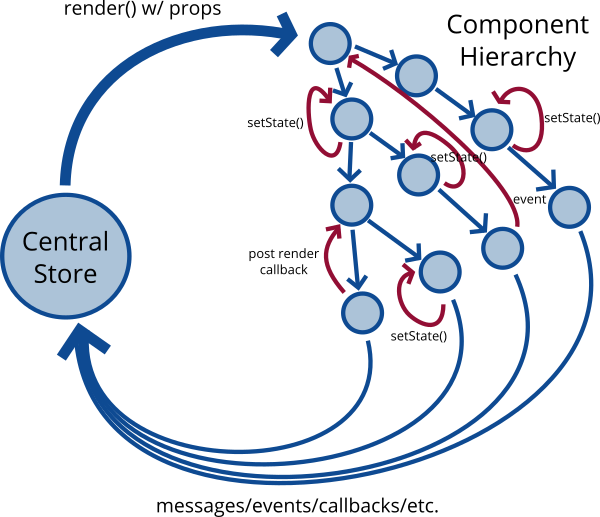
\includegraphics[scale=0.5]{obrazky/central_store}
\par\end{centering}
\caption{Diagram správy stavu aplikace pomocí frameworků React a Redux \cite{react_best_practices}} \label{fig:central_store}
\end{figure}
\FloatBarrier

\subsection{Jednosměrný tok dat}
Aplikace je vždy kompletně překreslena z virtuálního DOM při každé změně jejího stavu. Framework React používá jednosměrný tok dat – od vlastníka do vlastněné komponenty. Tento proces se opakuje rekurzivně dokud nejsou data aktualizována na všech místech. Tímto je zajištěna aktuálnost všech dat isomorfní webové aplikace. Komponenty přijímají data pouze v okamžiku vykreslování. Když se data změní, framework zajístí předání aktuálních dat a komponenta se vykreslí znovu. Tento princip si klade za cíl zjednodušit předávání dat v aplikaci \cite{react}.

\vspace{3mm}
\begin{figure}[h]
\begin{centering}
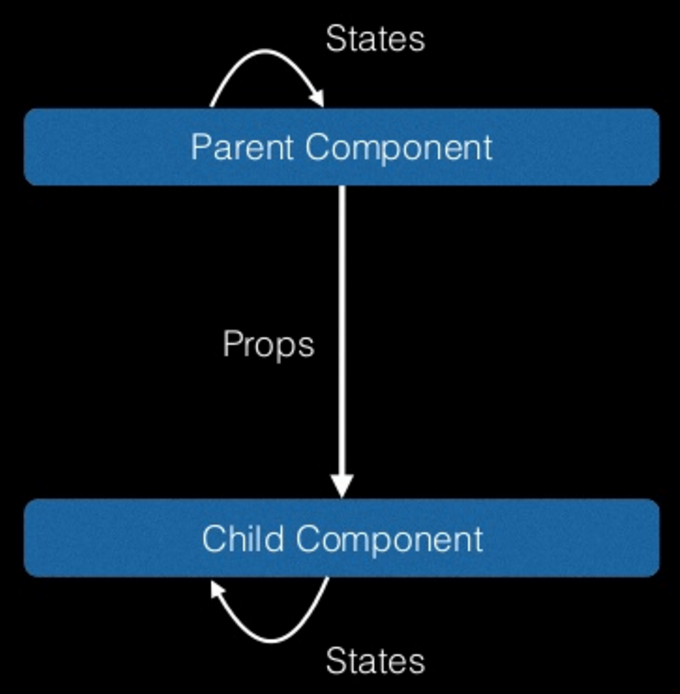
\includegraphics[scale=0.3]{obrazky/oneway_dataflow}
\par\end{centering}
\caption{Diagram jednosměrného toku data v React \cite{react} \label{fig:onewaydataflow}}
\end{figure}
\FloatBarrier

\subsection{Realtime komunikace a synchronizace}
Celá aplikace je velmi interaktivní a podporuje realtime komunikaci s databází. Přidání nové položky nebo její změna se okamžitě projeví u všech připojených uživatelů, bez nutnosti znovu načítat stránku. Doručení nových dat do webových prohlížečů je realizováno pomocí Websocketu, změny není nutné periodicky ověřovat, server změnu doručí sám, jakmile k ní dojde. Synchronizace stavu aplikace probíhá nejen mezi různými uživateli, ale pochopitelně také mezi více okny jednoho uživatele. Rychlé propagaci nových dat také pomáhá použitá databáze RethinkDB, která pomocí triggerů umožňuje notifikovat webovou aplikaci o změně uložených dat. Ta potom provede aktualizaci jejich zobrazení \cite{rethinkdb}. Použití této databáze je podrobněji popsáno v kapitole \hyperref[sec:rethinkdb]{5.3.7}. 

\section{Použité technologie}
Následující kapitola shrnuje technologie a související knihovny, které byly použity v ukázkové isomorfní webové aplikaci. U každé k knihoven je uveden její účel spolu se souvisejícím příkladem zdrojového kódu. Použitý kód pochází přímo z implementace ukázkové webové aplikace.

\subsection{node.js}
Node.js je základní předpoklad isomorfního přístupu, umožňuje zpracovávat javascriptový kód na serveru, a tím přináší serverové vykreslování šablon, které řeší mnohé problémy typických jednostránkových webových aplikací. To je popsáno v kapitole \hyperref[sec:node_js]{2.4}. Spolu s node.js se v ukázkové aplikaci používá také balíčkovací systém NPM, který řeší správu závislostí a spouštění obslužných skriptů vyvíjené aplikace \cite{nodejs} \cite{npm}.

\subsection{express}
Minimalistický framework Express je de facto standardizovaným serverovým frameworkem pro node.js. Ulehčuje definování aplikačních rozhraní, práci s databází a podobně. U isomorfních aplikací se především používá jako datové API. Je také plně kompatibilní s knihovnou React, kterou využívá při serverovém vykreslování šablon \cite{express}. Následující ukázka kódu popisuje definici dvou vstupních bodů API a příklad implementace server-side renderingu.

\begin{lstlisting}[language=Javascript,caption={Ukázka konfigurace serverového JS frameworku Express}]
var express=require('express');
var app = express();

app.get('/api/comments', function(req, res) {
  /* zpracovaní požadavku a vrácení dat */
});

app.post('/api/comments', function(req, res) {
    /* zpracovaní požadavku a vrácení dat */
});

app.get(['/'], function(req, res) { // server-side rendering
  /* Use React Router */
  var ReactRouter = require('react-router');
  var match = ReactRouter.match;
  var routes = require('./public/routes.js').routes

  match({routes: routes, location: req.url}, function(error, redirectLocation, renderProps) {
    /* vykreslení celé React aplikace a jeji vrácení jako čisté HTML */
  });
});
\end{lstlisting}

\subsection{React}
Framework React je knihovna pro tvorbu uživatelského rozhraní od společnosti Facebook. Je podrobně popsána v kapitolách \hyperref[sec:react]{2.8.3} a \hyperref[sec:react_isomoprhic]{4.4.5}.

Díky svému úzkému zaměření na vykreslování HTML, je vhodná pro použití v isomorfních aplikacích, protože bezproblémově běží v prohlížeči i na serveru \cite{react}. 

\subsubsection{Hlavní komponenta aplikace}
Následuje ukázka kódu hlavní React komponenty, která definuje celou webovou aplikaci. Je vidět použití komponent Header a Footer, reprezentujících společné části layoutu – hlavičku a patičku. Datové entity (komentáře) jsou hlavní komponentě předány pomocí props (viz \hyperref[sec:react_props]{2.4}). Pod komentáři se nachází formulář pro přidání nového komentáře. Tato komponenta představuje nejvyšší uzel stromu komponent, její změna tedy vyvolá překreslení celé webové aplikace. Tato ukázka představuje implementaci této komponenty v ukázkové webové aplikaci.
\begin{lstlisting}[language=Javascript,caption={Render metoda hlavní React komponenty GuestbookApp}]
  render() {
    let actions = { 
      editEvent: this.props.editEvent, 
      deleteEvent: this.props.deleteEvent
    };
    return (
      <div id="GuestbookApp">
        <Header/>
        <AsyncBar isWorking={this.props.isWorking} error={this.props.error} />
        {this.props.comments}
        <section className='container addCommentForm'>
          <CommentInput onSubmit={this.props.addEvent} userId={this.props.userId} textLabel='What happened?' authorLabel='Your nickname' valueLabel='Rating' />
        </section>
        <Footer/>
      </div>
    );
  }
\end{lstlisting}

\subsubsection{Datové komponenty}
Další skupinu komponent tvoří ty, která zobrazují data. Jedná se většinou o datové kontejnery, které zobrazují kolekce, nebo o jednoduché HTML komponenty vizualizující nějaká data. Syntaxe JSX, která kombinuje HTML a Javascript, dovoluje zobrazovat datové entity pomocí funkce \textit{map()}, která dostává definici datové komponenty jako argument. To umožňuje psát kratší a čitelnější kód, jak je vidět na příkladu níže. Na něm je také patrné řešení zástupného textu, pokud neexistují žádné komentáře.
\begin{lstlisting}[language=Javascript,caption={Render metoda datové komponenty CommentList pro zobrazení komentářů}]
render(){
   let list;
    if (comments.length > 0) {
      list = comments.map((event, key) =>
        <CommentItem key={key} row={key} id={event.id} editable={editable} event={event} {...actions} />
      );
    } else {
      list = <p>No comments!</p>;
    }
    return (
      <section className='container'>
        <div className='commentList'>
          <ul>
            {list}
          </ul>
        </div>
      </section>
    );
}
\end{lstlisting}

Na této ukázce kódu je vidět implementace jednoduché datové komponenty, která zobrazuje předaná data. Tvoří HTML reprezentaci některé z použitých datových entit, v našem případě se jedná o komentář. Ukázka také demonstruje princip jednotné zodpovědnosti, aby datová komponenta nemusela řešit mazání komentáře, dostává celou logiku nezbytnou pro mazání zvenčí jako property – \textit{ \{del\}} v ukázce (viz. \hyperref[sec:react_props]{2.4}).
\begin{lstlisting}[language=Javascript,caption={Render metoda komponenty CommentItem reprezentující komentář}]
render(){
  return (
     <div className='commentItem'>
          <p className='title'>
            {comment.text}
          </p><br/>
          {del}<br/>
          <p className='author'>
             Author: {comment.author}
          </p>
          <p className='created'>{moment(modified).fromNow()}</p>
     </div>
     );
}
\end{lstlisting}


\subsubsection{React router}
Velmi důležitou součástí každé webové aplikace je router, u isomorfních je nutné používat jeden router pro webový prohlížeč a druhý pro server. Díky možnostem moderního javascriptu však můžeme deklaraci routovacích pravidel extrahovat do vlastního souboru, který lze použít v obou routerech. V aplikaci se využívá React-router, jednotlivá pravidla se zapisují pomocí syntaxe JSX \cite{react_router}.
\begin{lstlisting}[language=Javascript,caption={Deklarace routovacích pravidel pomocí nástroje React-router}]
    <Route path='/' component={GuestbookApp}>
       <IndexRoute components={{comments: RecentComments}} />
       <Route path='all-comments' components={{comments: AllComments}} />
    </Route>
\end{lstlisting}

Knihovna React-router také poskytuje nástroje pro generování HTML odkazů na základě routovacích pravidel. Díky tomu není při tvorbě odkazů nutné používat HTML tag \textbf{a} a přemýšlet nad správným URL \cite{react_router}. Syntaxe je zřejmá z následující ukázky. 
\begin{lstlisting}[language=Javascript,caption={Využití generování HTML odkazů pomocí nástroje React-router}]
<ul>
	<li><Link to="/" activeStyle={{fontWeight: 'bold'}} onlyActiveOnIndex>Comments</Link></li>
	<li><Link to="/another-page" activeStyle={{fontWeight: 'bold'}}>Another Page</Link></li>
</ul>
\end{lstlisting}

\subsubsection{Čtení formulářových dat}
React také velmi usnadňuje tvorbu formulářů, pomáhá při jejich ověřování a řeší také odesílaní vstupních dat. Většinou se pro navěšování událostí na formulářové prvky používají klasické HTML atributy \textit{onClick}, \textit{onChange} a jim podobné. React ale nepoužívá oboustranný data binding \footnote{Data - binding poskytuje flexibilní mechanismus pro synchronizaci dat a uživatelského rozhraní.}, proto je nutné načíst formulářová data ručně \cite{react}. Tlačítko, které většinou řídí odesílání dat, musí získat přístup k HTML inputům, které drží data. Každá změna jakéhokoliv formulářového prvku fakticky vytváří nový stav související React komponenty, která ho zobrazuje. Často se proto používají takzvané \uv{watcher funkce}, které reagují na změnu formulářového prvku a jeho novou hodnotu ihned propagují do stavu příslušné komponenty. To je použito i v ukázkové aplikaci, implementace tohoto řešení je vidět na ukázce níže.
 
\begin{lstlisting}[language=Javascript,caption={Ukázka propagace hodnot formulářových polí do stavu React komponenty}]
  handleAuthorChange(e){ // handleTextChange je velmi podobná metoda
    this.setState({ author: e.target.value });
  }
  
  render(){
  ...  
  <textarea ... onChange={::this.handleTextChange}></textarea>
  <input ... onChange={::this.handleAuthorChange}/>
  ...
  }
\end{lstlisting}

\subsubsection{Server-side rendering}
Jednou se stěžejních technik isomorfního přístupu je server-side rendering, detailně popsaný v kapitole \hyperref[sec:server_side_rendering]{4.1.6}. Tento přístup umožňuje vygenerovat prvotní stav jednostránkové isomorfní aplikace na serveru pomocí node.js, což velmi urychluje načítání jednostránkových aplikací a tento prvotní stav se také zobrazí vyhledávacím robotům nebo uživatelům s vypnutým Javascriptem. Následující ukázka je demonstrací serverového vykreslení prvotního stavu webové aplikace.
\begin{lstlisting}[language=Javascript,caption={Ukázka propagování stavu aplikace ze serveru do prohlížeče }]
export function handleRender(req, res) {  
    // vytvoříme nový Redux store
    const store = createStore(rootReducer, {comments: initialComments, userId: 'baseUser'}); // userId bude vytvořeno až v prohlížeči

    // vykreslíme celou aplikaci do textu
    const html = React.renderToString(
      <Provider store={store}>
        {() => <GuestbookApp />}
      </Provider>
    );

    // odešleme vykreslenou aplikaci spolu s počátečním stavem do prohlížeče
    res.render('index', { html: html, initialState: JSON.stringify(store.getState()) });
}
\end{lstlisting}

Celá React aplikace se nejprve vykreslí do HTML pomocí serverového Javascriptu a spolu s počátečním stavem aplikace je odeslána do webového prohlížeče. Počáteční stav aplikace, který reprezentuje Redux store je serializován a uložen do proměnné \textit{window.\_\_INITIAL\_STATE\_\_}, ze které je pak store na klientské straně opět obnoven a celá aplikace spuštěna we webovém prohlížeči.

\begin{lstlisting}[language=Javascript,caption={Ukázka získaní počátečního stavu aplikace z webového prohlížeče}]
// získáme počáteční stav z globální promenně vygenerované serverem
let initialState = window.__INITIAL_STATE__;
const createStoreWithMiddleware = applyMiddleware(  
  thunkMiddleware,
  loggerMiddleware
)(createStore);

// vytvoříme z počátečního stavu Redux store
const store = createStoreWithMiddleware(actionReducers, initialState);

// překreslíme aplikaci v prohlížeči
React.render(  
  <Provider store={store}>
    {() => <GuestbookApp />}
  </Provider>,
  document.getElementById('app')
);

\end{lstlisting}
Serverové vykreslování nefunguje pouze pro úvodní stránku webové aplikace, server rozumí definicím klientských routovacích pravidel, takže načtení prvotního stavu a spuštění celé aplikace je možné na jakékoliv veřejně dostupné URL. Především díky tomu není indexování isomorfních aplikací žádný problém.

\subsection{Redux}
Isomorfní aplikace také přinesly novou architekturu zacházení s daty, známou jako Flux. Tento způsob práce s daty webové aplikace představila společnost Facebook a pojednává o něm kapitola \hyperref[sec:flux]{4.4.6}. Redux je v současné době preferovaná implementace tohoto návrhového vzoru. Při práci s Reduxem se používají tři základní konstrukce: \textit{store}, \textit{akce} a \textit{reducer}, který je mírně upravenou implementací dispatcheru popisovaného vzorem Flux \cite{redux}.

\subsubsection{Store}
Store tvoří \uv{srdce} celé isomorfní webové aplikace, jsou v něm uloženy veškerá data, stavy React komponent a některé další objekty. Store jako takový tvoří stav aplikace a existuje vždy právě jeden. Vytvořit ho pomocí nástroje Redux lze takto \cite{redux}:
\begin{lstlisting}[language=Javascript]
var store = Redux.createStore(reducer);
\end{lstlisting}

\vspace{3mm}
\noindent Store poskytuje tyto 3 základní metody, které řeší veškeré nezbytné operace \cite{redux}.
\begin{itemize}
\item store.getState() - vrací naše data (state)
\item store.subscribe(callback) – navěšení listener funkce na změnu store
\item store.dispatch(akce) – provádíme akci, která změní data ve store uložená
\end{itemize}

\subsubsection{Akce}
Pokud chceme provést změnu ve store (nebo obecně v aplikaci), je nutné tuto změnu realizovat pomocí jednoduchého objektu zvaného akce. Objekt akce má jediný povinný atribut zvaný \textit{type}, který slouží pro identifikaci akce reducerem při jejím vyhodnocování (viz níže). Jakékoliv další atributy jsou volitelné pro každou akci. Ta ale musí být jednoznačně identifikovatelná a musí obsahovat všechna data nutná k jejímu provedení.

\pagebreak
\noindent Příklady tří akcí v ukázkové webové aplikaci:
\begin{lstlisting}[language=Javascript, caption={Ukázka několika Redux akcí}]
{
    type: "ADD_COMMENT",
    text: "I really love your website!",
    author: "John Doe"
}
{
    type: "REMOVE_COMMENT",
    id: 15
}
{
    type: "REMOVE_ALL"
}
\end{lstlisting}

Tento objekt popisuje změnu dat, která bude provedena. Akcí popsaná změna se realizuje pomocí metody \textit{dispatch(akce)} nad store, která vyžaduje danou akci jako svůj jediný argument.

\begin{lstlisting}[language=Javascript, caption={Ukázka volání akce na Redux store}]
store.dispatch({ type: 'ADD_COMMENT', text: "I really love your website!", author: "John Doe" });
\end{lstlisting}

\subsubsection{Reducer}
Poslední nezbytnou součástí Reduxu je reducer, který akcemi definované modifikace dat provádí. Jedná se o obyčejnou funkci, která je součástí store a provádí bezpečné modifikace uložených dat vyjádřených pomocí výše popsaných akcí. V momentě zavolání metody \textit{dispatch()}, je spuštěna funkce reduceru, která od store přebírá tyto parametry \cite{redux}:
\begin{itemize}
\item state – současná data aplikace
\item action – celý objekt akce tak, jak jsme jej vložili do volání dispatch() (akce obsahuje identifikaci \textit{'type'} a jakákoliv další data potřebná k provedení)
\end{itemize}

Uvnitř reduceru je kód, který podle identifikace akce provede požadovanou změnu dat a vrátí jejich novou podobu (nový state).

\pagebreak
\begin{lstlisting}[language=Javascript,caption={Ukázka implementace Redux reduceru}]
if (action.type === "add") { 
    return addSomething(action.something); // zpracování akce přidat 
} else if (... //zde bude zpracování dalších akcí
} else return state; //pokud nebyla žádná akce provedena tak vracíme původní nezměněná data
\end{lstlisting}

Nový stav aplikace vždy vzniká z interakce původního stavu s objektem akce. Poslední větev cyklu if je zde pro případ, že store obsahuje více reducerů. Každou akci totiž dostanou všechny reducery a reagují na ni jen pokud je pro ně určena. V opačném případě reducer pouze vrátí nezměněný stav.

Při práci s daty aplikace také existuje jedno důležité pravidlo: \textbf{všechny modifikace dat provedené v reduceru musí být imutabilní}. Princip imutability je popsán v kapitole \hyperref[sec:immutability]{4.3} této práce. V praxi to znamená, že nelze provádět změnu stavu aplikace přímo. Nejprve je nutné si strukturu naklonovat, poté je možné na její kopii provést změny. Modifikovanou kopii aktuálního stavu pak předáme do store jako nový stav aplikace \cite{redux}.

\subsection{immutable.js}
Rychlost práce isomorfních webových aplikací do velké míry závisí na použití imutabilních objektů, které popisuje kapitola \hyperref[sec:immutability]{4.3}. Ukázková aplikace používá framework immutable.js od společnosti Facebook, který poskytuje sadu imutabilních datových struktur, které lze jednoduše používat \cite{immutablejs}. Popisovaná aplikace používá imutabilitu hlavně při práci s datovými entitami – komentáři. Následující ukázka ilustruje vytvoření imutabilních reprezentací komentářů v aplikaci.
\begin{lstlisting}[language=Javascript,caption={Ukázka vytváření imutabilních datových objektů v ukázkové aplikaci}]
import { Record } from 'immutable';

export const Comment = new Record({
    id: undefined,
    text: '',,
    author: undefined
});

let comments = api.getComments().forEach( comment -> new Comment(comment)); // pomocí new vytvoříme imutabilní reprezentace komentářů
\end{lstlisting}
\subsection{Babel}
Babel je transpiler Javascriptu, který umožňuje používat jeho moderní standard známý jako ES6 pro programování webových aplikací už dnes. Zprostředkovává překlad použitého kódu do starší verze Javascriptu, kterou podporuje většina současných prohlížečů. Babel také rozumí rozšířené syntaxi JSX, kterou používá framework React. Nástroj je podrobněji popsán v kapitole \hyperref[sec:babel]{2.3.2}. Jeho základní funkcionalitu lze rozšířit pomocí balíčků, dostupných pomocí NPM \cite{babel}.

\vspace{3mm}
\noindent Rozšiřující Babel balíčky použité v ukázkové aplikaci:
\begin{itemize}
\item babel-core – jádro Babel,
\item babel-loader – integrace knihovny Babel do webpacku,
\item babel-preset-es2015 – preset Babelu pro překlad do ES5,
\item babel-preset-react – rozšíření Javascriptu pro podporu knihovny React,
\item babel-plugin-transform-class-properties – toto rozšíření navíc přidává, proměnné a konstanty ve třídách.
\end{itemize}

\subsection{RethinkDB}
\label{sec:rethinkdb}
RethinkDB je opensource distribuovaná databáze, která ukládá dokumenty ve formátu JSON. Byla vyvinuta s ohledem na potřeby moderních webových aplikací. Mezi její hlavní výhody patří \cite{rethinkdb}: 

\begin{itemize}
\item vlastní výkonný dotazovací jazyk,
\item jednoduché škálování,
\item distribuovaný návrh,
\item možnost realtime spojení s aplikací, okamžitá propagace změn,
\item výborná dokumentace a mnoho aktuálních příkladů.
\end{itemize}

V práci je použita především díky možnosti definice triggerů, které zajišťují aktualizaci zobrazení dat všech uživatelů v reálném čase. Následující ukázka kódu demonstruje použití takového triggeru \cite{rethinkdb}.

\begin{lstlisting}[language=Javascript,caption={Použití triggeru v databázi RethinkDB}]
export function liveUpdates(io) {
  console.log('Setting up listener...');
  connect()
  .then(conn => {
    r
    .table('pulses')
    .changes().run(conn, (err, cursor) => { // navěšení funkce triggeru
      console.log('Listening for changes...');
      cursor.each((err, change) => {
        console.log('Change detected', change);
        io.emit('event-change', change); // vyvolání události v připojených prohlížečích
      });
    });
  });
}
\end{lstlisting}

\subsection{Webpack}
Webpack představuje nástroj pro automatizaci vývoje webových aplikací, nazývaný \textit{module bundler}. Ten v podstatě za základě závislostí z několika vstupních souborů vygeneruje jeden výstupní soubor. Svým použitím fakticky nahrazuje task runnery, jejichž filozofie je ale značně odlišná a některé operace tak nelze řešit pomocí Webpacku. Je tedy obvyklé na složitějším projektu používat Webpack například spolu s Gulpem.

Module bundler Webpack zpracovává jak javascriptové soubory, tak i styly nebo obrázky. Také řeší překlad javascriptového kódu pomocí Babelu, zpracování CSS preprocesorů, nebo umí využívat NPM knihovny i v prohlížeči. Podrobně je tento nástroj popsán v kapitole \hyperref[sec:webpack]{4.4.7}.

\begin{lstlisting}[language=Javascript, caption={Ukázka konfigurace Babel-loaderu pro webpack}]
module: {
      loaders: [
          {
              test: /\/src\/.+\.js$/,    //pro všechny soubory v adresáři src s koncovkou js...
              loader: 'babel-loader',  //použij babel-loader
              query: {
                  presets: ['react', 'es2015'], //vybrané babel presety: 
                  plugins: ["transform-class-properties", "react-hot-loader",...] //vybrané pluginy 
              }
          }
    ]
}
\end{lstlisting}

Ukázková webová aplikace používá několik pluginů pro Webpack. Nejzajímavějším z nich je \textit{React Hot Loader}, který zpříjemňuje vývoj webové aplikace tím, že dokáže aktualizovat definice React komponent za běhu aplikace. Použitý byl také \textit{babel-loader}, \textit{stylus-loader} nebo \textit{image-loader}. Funkce těchto pluginů je zřejmá z jejich názvů.

\subsection{Stylus}
Stylus je CSS preprocesor, který se od ostatních známých liší především tím, že používá takzvanou \uv{whitespace syntaxi}. Kód Stylusu nepoužívá žádné závorky ani středníky, jednotlivé bloky jsou uvozeny pouze odsazením. Nástroj také přináší možnost definice proměnných a další věci, které CSS preprocesory běžně nabízejí \cite{stylus}.

\begin{lstlisting}[caption={Ukázka stylování v jazyce Stylus}]
body
  font: 12px Helvetica, Arial, sans-serif;

a.button
  -webkit-border-radius: 5px;
  -moz-border-radius: 5px;
  border-radius: 5px;
\end{lstlisting}

\section{Komunikace}
Moderní webové aplikace jsou obecně postaveny na časté komunikaci prohlížeče s webovým serverem, je třeba získávat stále nová data nebo části HTML. Aplikace v Javascriptu komunikují se serverem buď prostřednictvím klasických HTTP požadavků nebo pomocí nové technologie Websocket. S její pomocí lze navázat obousměrné spojení, kde klient (webový prohlížeč) může komunikovat se serverem v reálném čase. Není tak nutné používat techniku zvanou \textit{heartbeat}, kdy se klient v pravidelných intervalech dotazuje serveru jestli existují změny. To znamená, že také server má možnost komunikovat s připojenými prohlížeči, může tedy posílat nová data ihned, jakmile vzniknou. S Web Sockets je mnohem snažší vytvářet realtimové aplikace, jako jsou online chaty či kooperativní služby. Jeho použití zefektivní a zrychlí každou webovou aplikaci \cite{websocket}. Data se většinou odesílají ve formátu JSON, který je standardizovaným serializérem v Javascriptu \cite{json}.

Ukázková webové aplikace používá framework Socket.io, který usnadňuje obsluhu Websocket komunikace \cite{socketio}. Následující ukázka zobrazuje propojení serverem vyvolané události s reakcí realizovanou změnou stavu Redux store.
\begin{lstlisting}[language=Javascript,caption={Ukázka propojení Websocketu s Redux store}]
  const io = socketClient();

  io.on('event-change', (change) => {   // pokud dojde k události comment-change
    let state = store.getState();
    // rozhodneme co se stalo a zavoláme příslušnou akci na store
    if (!change.old_val) {
      store.dispatch(actions.addCommentSuccess(change.new_val));
    } else if (!change.new_val) {
      store.dispatch(actions.deleteCommentSuccess(change.old_val));
    } else {
      store.dispatch(actions.editCommentSuccess(change.new_val));
    }
  });
\end{lstlisting}

\section{Sestavování a spouštění aplikace}
Popisovaná webová aplikace nepoužívá žádný specializovaný task runner typu Grunt či Gulp, místo toho si vystačí s operacemi, které lze definovat v NPM. Balíčkovací systém umožňuje definovat úkoly, které se potom volají pomocí příkazu \textit{npm run NAZEV\_AKCE} \cite{npm}. Jejich definice jsou uloženy v souboru package.json pod klíčem \textit{scripts} viz ukázka.

\begin{lstlisting}[language=Javascript,caption={Definice vlastních operací nad projektem pro NPM v souboru package.json}]
  "scripts": {
    "build:prod": "NODE_ENV=production webpack",
    "db-setup": "node dbSetup.babel.js",
    "lint": "eslint client server universal test server.js dbSetup.js",
    "start": "NODE_ENV=development node start-dev.js",
    "start:win": "set NODE_ENV=development&&node start-dev.js",
    "start:prod": "NODE_ENV=production node server.babel.js",
    "test": "./node_modules/karma/bin/karma start"
  },
\end{lstlisting}

Jak je vidět z ukázky, každá definice úkolu v NPM je pouze jakýsi zástupce pro jiný příkaz, většinou využívající node.js. Volání \textit{npm run start} je tedy ekvivaletní s voláním \textit{NODE\_ENV=development node start-dev.js}. Vše co je možné provést z příkazové řádky, je možné definovat jako úkol v NPM \cite{npm}. 

\vspace{3mm}
\noindent NPM úkoly implementované v ukázkové webové aplikaci:
\begin{itemize}
\item \textbf{build:prod} – vytvoření balíčku aplikace pro nasazení na server,
\item \textbf{db-setup} – připravení databáze pro vývoj,
\item \textbf{lint} – lintování kódu,
\item \textbf{start} – spuštění aplikace ve vývojovém módu,
\item \textbf{start:prod} – spuštění aplikace v produkčním módu,
\item \textbf{test} – spuštění testů.
\end{itemize}

\section{Struktura aplikace}  
\begin{figure}[h]
\begin{centering}
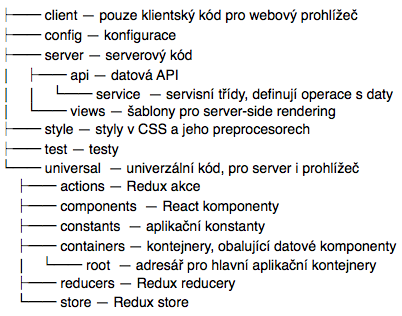
\includegraphics[scale=0.6]{obrazky/struktura}
\par\end{centering}
\caption{Adresářová struktura ukázkové webové aplikace \label{fig:structure}}
\end{figure}
\FloatBarrier
          
\subsection{Vstupní body aplikace}              
Ukázková aplikace obsahuje dva vstupní body, tedy soubory ze kterých je spuštěna inicializace webové aplikace. Každý z nich je určený pro odlišné prostředí, jeden pro server a druhý po prohlížeč. Oba dva v podstatě spouští totožnou aplikaci, ale při použití isomorfního přístupu je jejich použití nezbytné. Jedná se o soubory:
\begin{itemize}
\item \textbf{server.js} – nastartuje webový server v node.js, který zpracovává HTTP požadavky na API a spouští serverové vykreslování požadované šablony.
\item \textbf{client/app.js} – spustí se v prohlížeči při prvním načtení webové aplikace, pokud je povolený Javascript. Aplikace si načte prvotní stav předaný serverem a spustí celou klientskou část aplikace, ta je po kompletním načtení plně zodpovědná za další obsluhu.
\end{itemize} 

\subsection{Sdílený kód}
Isomorfní kód, neboli univerzální Javascript je uložen v adresáři \textit{universal}. Ten obsahuje definici routování, všechny React komponenty nebo kompletní definici obsluhy dat dle architektury Flux. Tu v naší ukázkové aplikaci realizuje nástroj Redux, jehož komponenty jsou uloženy ve složkách \textit{actions}, \textit{reducers} a \textit{store}. Komponenty uživatelského rozhraní jsou v aplikaci dvou typů. Tím prvním jsou klasické React komponenty, zobrazující nějaká data, nebo reprezentující společné části HTML layoutu. Ty jsou uloženy v adresáři \textit{components}. Druhý typ jsou takzvané \uv{kontejnerové komponenty}. Ty v kontextu frameworku React většinou tvoří jednak samotnou webovou aplikaci (hlavní komponenta) nebo se používají pro zobrazování kolekcí. Kontejnery používají vlastní složku \textit{containers}. Poslední důležitou části sdíleného kódu jsou routovací pravidla, ty jsou definována pomocí JSX pro nástroj React-router a uložena v souboru \textit{routes.js}. Tento soubor také importuje serverová část aplikace, kvůli nutnosti routování požadavků také na serveru.

\subsection{Serverová část}
Serverová část aplikace využívá framework Express a řeší vedle datového API také vykreslování samotné React aplikace, respektive ve většině případů jenom jejího prvotního stavu. Je definována v souboru server.js v kořenovém adresáři aplikace.
\begin{lstlisting}[language=Javascript, caption={Ukázka serverové části isomorfní webové aplikace}]
// servírování statického obsahu (obrázky, CSS, apod.)
app.use(require('serve-static')(path.join(__dirname, config.get('buildDirectory'))));

// definice API
app.get('/api/0/events', api.getEvents);
app.post('/api/0/events', api.addEvent);
app.post('/api/0/events/:id', api.editEvent);
app.delete('/api/0/events/:id', api.deleteEvent);

// favicon
app.get('/favicon.ico', (req, res) => res.sendFile(path.join(__dirname, 'images', 'favicon.ico')));

// definice metody pro serverove vykreslovani
app.get('*', uni.handleRender);
\end{lstlisting}

Syntaxe je velmi jednoduchá, nad Express objektem app existují funkce \textit{get}, \textit{post} a další, které reprezentují jednotlivé HTTP metody. Ty vždy přijímají dva argumenty, URL na kterém naslouchají a obslužnou funkci, které HTTP požadavek předají. Příklad ilustruje definici API, nastavení servírování statických souborů a hlavně také isomorfní server-side rendering. Ten provádí funkce \textit{handleRender()}. Ta provede na jakékoliv URL, které neodpovídají jiné definice, serverové vykreslení celé isomorfní webové aplikace. Tato funkce vyhodnotí URL a za základě routovacích pravidel získaných ze sdíleného kódu, vykreslí celou javascriptovou aplikaci na serveru a vrátí zpracované HTML, které poté klientská část načte a celou webovou aplikaci spustí v prohlížeči.
\subsection{Klientská část}
Klientskou část tvoří standardní React aplikace v Javascriptu. Její spuštění ilustruje tato ukázka kódu.
\begin{lstlisting}[language=Javascript, caption={Ukázka klientské části isomorfní webové aplikace}]
import routes from '../universal/routes';
import store from '../universal/store';
import * as actions from '../universal/actions/GuestbookActions';

import Root from '../universal/containers/root';

import '../style/pure.css';
import '../style/main.styl';
import '../style/spinner.styl';

const history = syncHistoryWithStore(browserHistory, store);

ReactDOM.render(
  <Root store={store} routing={routes} history={history} />,
  document.getElementById('app')
);
\end{lstlisting}

Využívá se universální kořenová Root komponenta, která přijímá Redux store, a instanci React routeru. Na základě předaných routovacích pravidel a aktuální URL dojde k vykreslení související kontejnerové komponenty. Zajímavosti je definice stylů pomocí příkazu \textit{import}, a to jak samotného CSS tak i stylopisů využívající preprocesor Stylus. O jejich načtení a zkompilování se postará module bundler webpack.

\begin{lstlisting}[language=Javascript, caption={Ukázka implementace kořenové React komponenty}]
export default class Root extends Component {
  render() {
    const { store, routing, history } = this.props;
    return (
      <Provider store={store}>
        <div>
          <Router history={history}>
            {routing}
          </Router>
        </div>
      </Provider>
    );
  }
};
\end{lstlisting}

\subsection{Testy}
Testy jsou v ukázkové aplikaci uloženy v adresáři \textit{test}. Jsou implementovány testy akcí a reducerů nástroje Redux. Při testování akcí ověřujeme, zda volání nějaké metody vytvoří správné Redux akce se správnými atributy. Testování reducerů má zase za úkol ověřit správnost mutace aplikačního stavu, jehož změny mají reducery na starost. Následuje ukázka jednoduchého testu akcí při získávání komentářů z API. Test kontroluje vznik akcí \textit{LOAD\_COMMENTS\_REQUEST} a \textit{LOAD\_COMMENTS\_SUCCESS} s příslušnou strukturou.
\begin{lstlisting}[language=Javascript, caption={Ukázka asynchronního testu získávání datových entit – komentářů}]
  describe('loadComments', () => {
    const mockStore = configureStore([thunk]);
    it('should trigger a LOAD_COMMENTS_REQUEST and LOAD_COMMENTS_SUCCESS action when succesful', () => {
      let requestMock = {
        get: () => ({
          set: () => ({
            end: (x) => x(null, {
              body: [ { name: 'Awesome', author: 'John Doe' } ]
            })
          })
        })
      };
      actions.__Rewire__('request', requestMock);
      let expectedActions = [
        { type: 'LOAD_COMMENTS_REQUEST' },
        { type: 'LOAD_COMMENTS_SUCCESS', events: [ { name: 'Awesome', author: 'John Doe' } ] }
      ];
      
      let initialState = {guestbookApp: { comments: [], userId: 'baseUser'} };
      let store = mockStore(initialState);

      store.dispatch(loadComments());
      const actualActions = store.getActions();
      expect(actualActions).to.eql(expectedActions);
    });
\end{lstlisting}


\chapter{Porovnání s existujícími vývojovými postupy}
Isomorfní přístup k programování webových aplikací je relativně nový princip, který přináší použití Javascriptu pro webový prohlížeč i webový server. Použití jednoho jazyka pro obě prostředí přináší mnoho výhod, je možné vyvíjet veškerý kód v jednom projektu, používat stejné knihovny nebo dokonce sdílet kód mezi jednotlivými prostředími. Nejdůležitější technologií, která isomorfní přístup umožnila, bylo bezesporu node.js. To přineslo možnost zpracovávat Javascript také na serveru. Využití Javascriptu na serveru také řeší většinu problémů jednostránkových aplikací, použití isomorfního přístupu je tedy ideální při vývoji velmi interaktivní aplikace. Je všeobecně známo, že jsou běžné jednostránkové aplikace nevhodné pro vývoj webu, kde je nezbytná dobrá indexovatelnost internetovými vyhledávači. Obecně se proto nedoporučuje programovat jako SPA obsahově založené weby, například magazíny nebo blogy. Použití isomorfního Javascriptu tento problém řeší a umožňuje tak naprogramovat jako SPA jakýkoliv web. Následující dva diagramy dobře ilustrují rozdíly v architektuře klasických a isomorfních jednostránkových webových aplikací.

\vspace{0,3cm}
\begin{figure}[h]
\begin{centering}
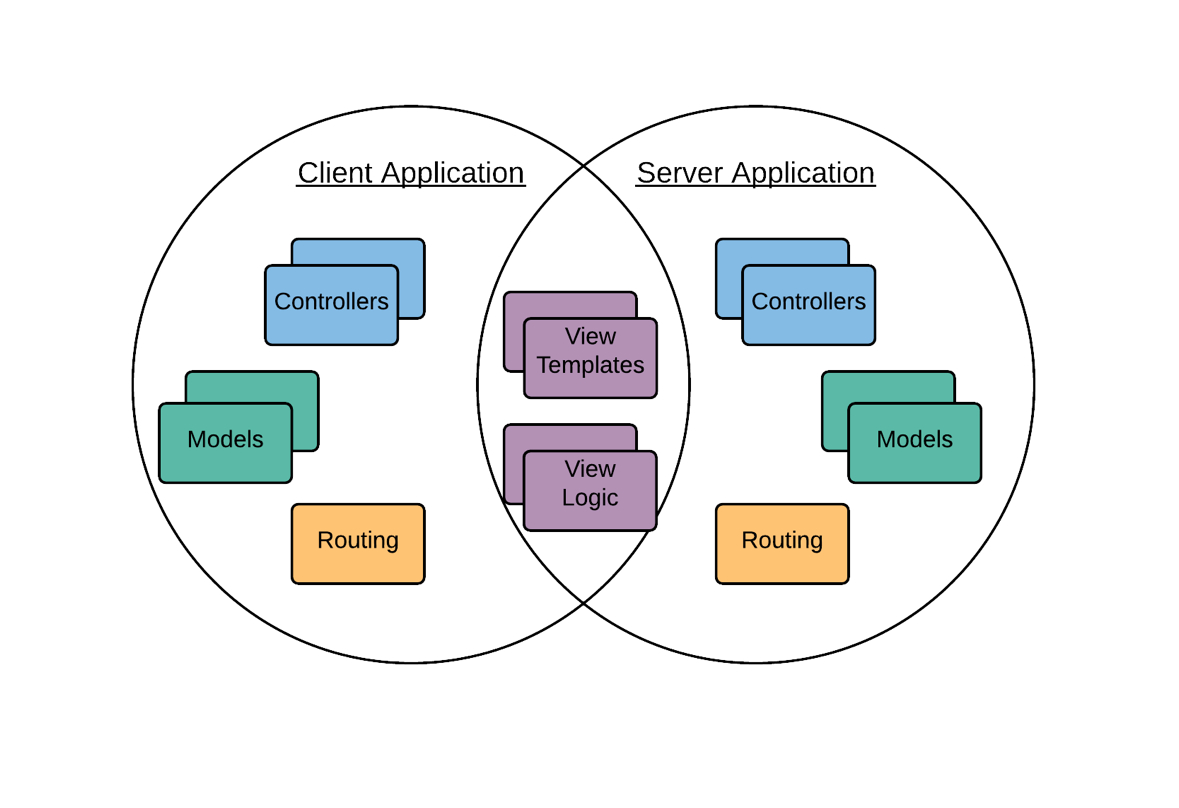
\includegraphics[scale=0.4]{obrazky/sharing_view}
\par\end{centering}
\caption{Diagram archiktuktury běžné jednostránkové aplikace \cite{isomorhic_book} \label{fig:spa_arch}}
\end{figure}

Běžné jednostránkové webové aplikace striktně oddělují serverovou a klientskou část aplikace. V době jejich vzniku to bylo považováno za výhodu, protože takové rozdělení aplikace zjednodušuje vývoj a umožňuje snadno vytvářet další klienty, například mobilní aplikace. Časem se však projevily problémy a nedostatky tohoto řešení. Koncept isomorfních aplikací proto opět spojuje serverovou a klientskou část a díky použití stejného jazyka umožňuje také sdílení kódu.

\begin{figure}[h]
\begin{centering}
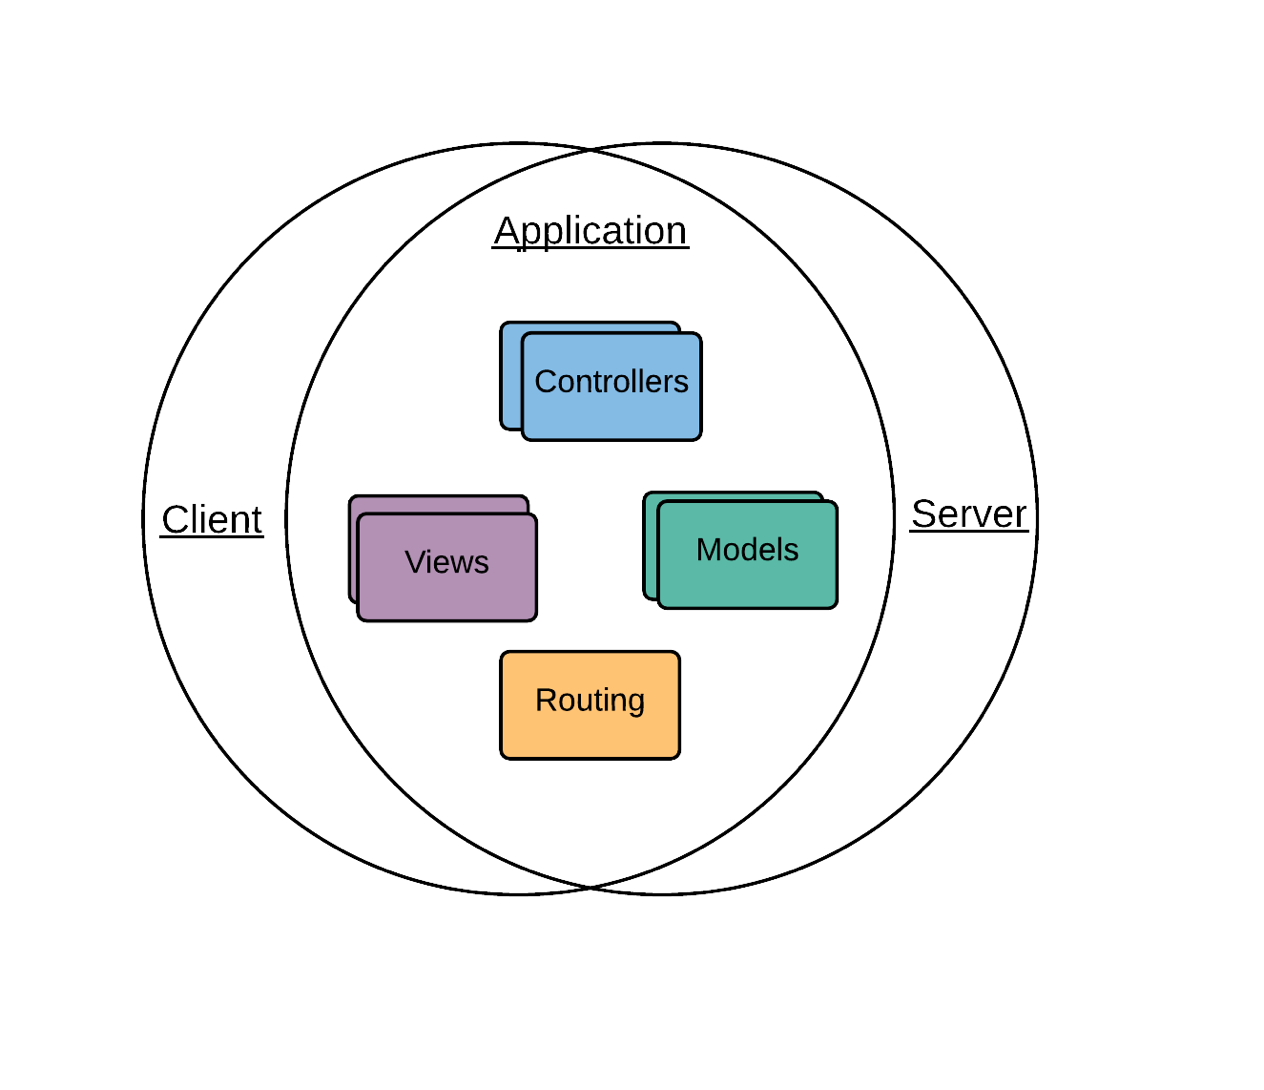
\includegraphics[scale=0.4]{obrazky/sharing_all}
\par\end{centering}
\caption{Diagram architektury isomorfní webové aplikace \label{fig:isomorphic_arch}}
\end{figure}
\FloatBarrier

Isomorfní webové aplikace sdílejí základní programové komponenty mezi serverem a prohlížečem. To je možné jen při použití stejného jazyka pro obě prostředí, kterým dnes může být jen Javascript. Isomorfní přístup konečně přináší plně indexovatelné jednostránkové webové aplikace. Porovnáme-li složitost implementace isomorfní aplikace s běžnou SPA, napsanou například v AngularJS, zjistíme, že se velmi liší. Je to dáno především specifickou syntaxí AngularJS a na druhé straně použitím jiných přístupů a nové syntaxe ES6 v React. Programátor je tak nucen osvojit si některé zcela nové přístupy, jinou syntaxi a některé specifické návrhové vzory. Jejich použití je ale dnes již do značné míry standardizované, můžeme tedy očekávat, že se budou v Javascriptu používat i za několik let. 

Eric Mathiason se ve své práci mimo jiné zaměřil na porovnání knihoven vhodných pro isomorfní přístup s klasickými SPA frameworky. Jeho práce porovnává frameworky React a Ember.js. Ember byl vybrán především proto, že není tolik komplexní jako například Angular, a tak se lépe hodí pro srovnání s React, který řeší především obsluhu uživatelského rozhraní. Následující tabulka shrnuje vlastnosti těchto frameworků \cite{mathiasson-isomorphic}.
\begin{table}[h]
\centering
	\caption{Srovnání javascriptových frameworků React a Ember.js \cite{mathiasson-isomorphic}}
	\begin{tabular}{ |p{6.5cm}|C{1.5cm}|C{1.5cm}| }
	\hline
	& React & Ember.js \\ \hline
	Podpora pro implementaci SPA & ANO & ANO \\ \hline
	Možnost serverového vykreslování & ANO & NE \\ \hline
	Použití vlastního šablonovacího jazyka & ANO & ANO \\ \hline
	Nízký průměrný čas načítání & ANO & NE \\ \hline
	REST komunikace & ANO & ANO \\ \hline
	Jednosměrný tok dat & ANO & NE \\ \hline
    \end{tabular}
	\label{tab:react_vs_ember}
\end{table}
\FloatBarrier

Mathiason se také zaměřil na srovnání rychlosti vykreslování javascriptové aplikace využívájící React a Ember.js. V tomto testu nebylo využito serverové vykreslování, které by dobu načítání React aplikace ještě snížilo \cite{mathiasson-isomorphic}.

\begin{figure}[h]
\begin{centering}
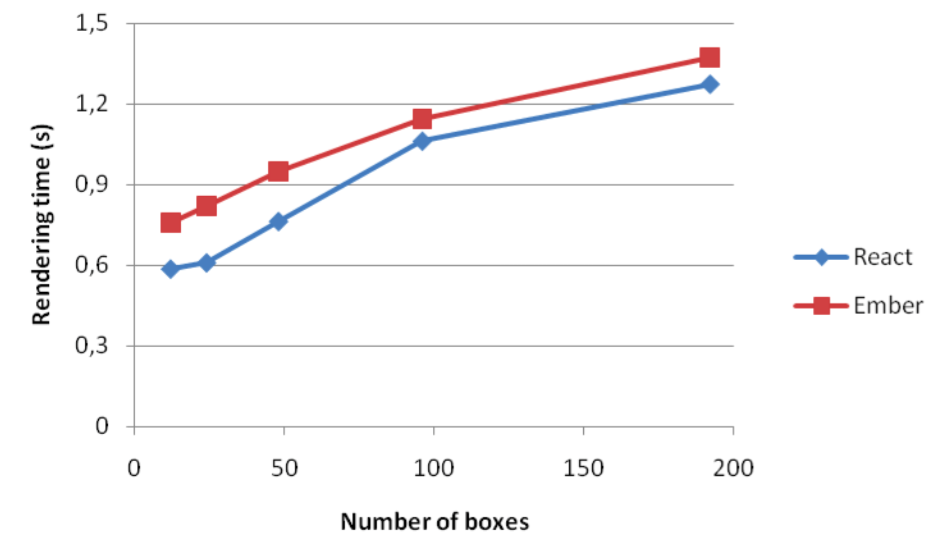
\includegraphics[scale=0.4]{obrazky/comparison_1}
\par\end{centering}
\caption{Porovnání rychlostí vykreslování frameworků React a Ember.js \cite{mathiasson-isomorphic} \label{fig:comparison_2}}
\end{figure}
\FloatBarrier

Porovnat isomorfní aplikace s klasickými serverově orientovanými frameworky, který používají Javascript jen okrajově, je složité. Především proto, že chování čistě serverové aplikace je značně odlišné od chování aplikace založené na Javascriptu. Serverové aplikace například neposkytují takovou interaktivitu jakou obecně jednostránkové aplikace nabízejí. Implementace vysoce dynamických aplikací ale bývá složitější především kvůli některým vlastnostem jazyka Javascript. Určitou zvláštností javascriptového vývoje je také používání velkého množství knihoven a z toho vycházející nutnost jejich konfigurace, která může být často složitá. V tomto prostředí začíná klesat popularita ucelených frameworků, na úkor velmi modulárních řešení, poskládaných z mnoha malých knihoven. Místo výrazu framework se v Javascriptu dnes často používá pojem \textit{devstack}. Jedná se o připravený soubor knihoven, tvořící kompletní vývojové prostředí. Dobře nakonfigurovaný devstack potom zastává funkce velkého monolitického frameworku známého z ostatních programovacích jazyků. Navíc však myslí i na pohodlí vývojáře. Devstacky pro vývoj isomorfních webových aplikací často podporují \textit{hot reloading}, což znamená okamžité doručování aktuální verze zdrojového kódu do webového prohlížeče. Každá změna ve zdrojovém kódu se okamžitě projeví v prohlížeči. Okamžitá propagace změn je velkým specifikem isomorfního přístupu. V jiných jazycích je nutné vyvíjené aplikace často restartovat, Javascript lze díky jeho návrhu modifikovat za běhu, nutnost restartování webové aplikace tedy odpadá a díky nástrojům jako Webpack, nemusí vývojář provádět ani obnovení samotné webové stránky ve webovém prohlížeči \cite{webpack}.

\chapter{Výsledky}
Práce si kladla za cíl především představit isomorfní přístup jako vhodnou techniku pro programování moderních webových aplikací. Tento přístup byl také porovnán s jinými zažitými principy vývoje. Isomorfní webové aplikace jsou v podstatě dalším evolučním stupněm vývoje jednostránkových webových aplikací v jazyce Javascript. Oproti klasickým jednostránkovým webovým aplikacím, které běží kompletně v prohlížeči, je implementace isomorfní aplikace o něco málo náročnější. Při použití vhodných nástrojů, které jsou navrženy pro běh v prohlížeči nebo node.js, je složitost vývoje isomorfních aplikací srovnatelná s běžnými SPA. Implementace klasických serverově orientovaných aplikací je samozřejmě jednodušší, především díky zažitým komplexním frameworkům a mnoha příkladům, které jejich vývoj velmi usnadňují. V poslední době ale popularita čistě serverových aplikací stále klesá. Vysoká interaktivita bývá základním požadavkem čím dál tím více webových aplikací, proto se stává isomorfní přístup stále populárnější. Jeho použití se vyplatí pro většinu typů aplikací, velmi totiž vylepšuje výslednou uživatelskou přívětivost aplikace a díky obnovování jen určitých částí stránky, také její intuitivnost. Určitou komplikací vývoje moderních webových aplikací v Javascriptu je velká dynamičnost vývoje používaných knihoven. Často vycházejí nové verze, přinášející mnoho změn, některé z nich mohou být také \textit{breaking changes}, tedy takové změny, které nejsou kompatibilní se starší verzí dané knihovny. To je dáno především tím, že většina knihoven určených pro isomorfní vývoj je stará pouze několik let a celé jejich rozhraní tak ještě není ustáleno. Řešením je definice přesných verzí knihoven v souboru \textit{package.json} a větší opatrnost při jejich upgradování.

Využití isomorfního přístupu je v podstatě nezbytné, tvoří-li programátor obsahově založenou webovou stránku, například zpravodajský server, diskuzní fórum, nebo jakoukoliv jinou webovou aplikaci, ke které se přistupuje převážně z internetového vyhledávače. Alespoň některý její obsah tedy má být veřejný. Jako klasické SPA se často vyvíjejí uzavřené informační systémy, kde se jejich nevýhody prakticky neprojevují. Tyto systémy totiž většinou vyžadují přihlášení a jejich obsah nemá být veřejně dostupný. I pro ně je ale isomorfní přístup vhodný a vzhledem k tomu, že celý přístup je fakticky evolucí vývoje v Javascriptu, lze očekávat že se jeho pomocí budou vytvářet všechny webové aplikace v Javascriptu. V současnosti jsou nejpoužívanější vývojové nástroje od společnosti Facebook, které z nich se ale nakonec stanou standardem, ukáže až čas.

Praktickým výsledkem této diplomové práce je ukázková isomorfní webová aplikace, na které jsou demonstrovány popisované přístupy. Vytvořená aplikace funguje ve většině internetových prohlížečů na běžném počítači, mobilním telefonu nebo tabletu. Aplikace je přínosná tím, že ukazuje moderní postupy při tvorbě interaktivních webových aplikací. Přínosem práce je také to, že se jedná o první akademickou práci zabývající se vývojem isomorfních webových aplikací vydanou v České republice.

\chapter{Závěr}
Javascript je v současné době bezpochyby jedním z nejpoužívanějších jazyků vůbec. Tvoří důležitou část kódu v nepřeberném množství různých druhů moderních webových aplikací a stále nachází nové možnosti nejen na straně klienta, ale i na straně serveru. Vývojových prostředí a nástrojů pro ladění použitelných pro práci s Javascriptem je velké množství. Liší se od druhu zvolené implementace a většina je jich navržena pro použití Javascriptu na webu, ale začínají se objevovat také serverově nebo mobilně zaměřené nástroje. Velkým pokrokem byl také příchod konceptu jednostránkových webových aplikací (SPA), který přinesl kompletní implementaci aplikační logiky webové aplikace v prohlížeči pomocí Javascriptu.

V práci jsou představeny Single Page Aplikace, jejich princip a technické řešení spolu se souvisejícími technologiemi, které umožnily vývoj webových aplikací na této architektuře. Takové aplikace jsou potom naprosto závislé na podpoře Javascriptu, což přináší několik zásadních nevýhod. Největší z nich je špatná indexovatelnost SPA, protože roboti internetových vyhledávačů nepodporují Javascript. Tím pádem nevidí na stránce žádný text. Koncept isomorfních aplikací přenáší část zodpovědnosti z webového prohlížeče na webový server. Ten je zodpovědný především za vykreslování HTML, vyhledávací robot díky tomu získá již částečně zpracovanou stránku, která již obsahuje textový obsah. 

Vývoj isomorfních aplikací vyžaduje komplexnější architekturu a složitější vývojové prostředí než u klasických SPA. Jednostránkové webové aplikace často používají jeden monolitický framework, například Angular.js, zatímco ty isomorfní často využívají dokonce desítky menších knihoven, které vždy řeší jenom jednu oblast vývoje. Největší problém isomorfních aplikací je řešení přenosu prvotního aplikačního stavu vygenerovaného serverem do klientské části, běžící ve webovém prohlížeči. Tento princip se nazývá \textit{redyhratace} a často se řeší pomocí serializace vygenerováno stavu do javascriptové proměnné, kterou načte webový prohlížeč a následně celou aplikaci spustí. Toto řešení je použité také v ukázkové aplikaci, která je součástí této práce. Zjednodušeně tím dosáhneme toho, že načítání aplikace v prohlížeči začne přesně od bodu, kde skončilo serverové vykreslování. Druhým problémem je distribuce dat v aplikaci, není totiž možné používat automatický obousměrný data binding, tolik známý z frameworku Angular.js. To vyřešila společnost Facebook pomocí návrhového vzoru Flux, který řeší efektivní správu, aktualizaci dat a propagaci jejich změn. Isomorfní aplikace tedy představují evoluci jednostránkových aplikací, která řeší jejich hlavní problémy a zachovává vysoký stupeň interaktivity. Implementační rozdíly jsou však značné, především kvůli použití nového standardu Javascriptu zvaného ES6. Syntaktických změn je mnoho, jsou ale dobře popsány a jejich osvojení je pro schopného programátora otázka několika dní. Cílem práce bylo především popsat isomorfní přístup k programování webových aplikací v Javascriptu. Práce také demonstrovala využití těchto principů pomocí vytvořené ukázkové aplikace.

Existují však také názory, že isomorfní aplikace jsou přesně proti proudu doby. Je všeobecně známo, že každý programovací jazyk je vhodný pro trochu jiný typ aplikace. Z toho vyplývá, že by bylo vhodné využívat více programovacích jazyků pro různé oblasti vývoje. Například Jiří Knesl říká: \uv{Vázat se na jeden jazyk je hloupé. Správné řešení je použít tolik jazyků, kolik se vyplatí, ale zároveň nezbytné minimum} \cite{knesl}. Isomorfní přístup ale souvisí pouze s webovými aplikacemi, kde je dle mého názoru využití jednoho jazyka pro prohlížeč i server více než vhodné.

\section{Další směry výzkumu v oblasti}
Princip vývoje isomorfních webových aplikací je starý pouze několik let a stále se dynamicky vyvíjí. Mnoho přístupů není ještě plně standardizovaných. V této práci bylo cílem popsat pouze celkem ustálené a často používané principy. Tedy ty problémy, které byli ve světě isomorfních aplikací takřka vyřešeny. Další problémy se aktuálně řeší, komunita kolem isomorfních aplikací mimojiné přemýšlí například o nejvhodnějším způsobu definice CSS stylů. Vývojáři používající framework React doporučují deklarovat styly Javascriptem každému elementu zvlášť pomocí atributu \textit{style} (inline styly) \cite{react_css}, zatímco jiní vývojáři od tohoto přístupu odrazují \cite{inline_styles_hate}. 

Lze také očekávat větší zapojení Javascriptu do vývoje na mobilních zařízeních, především díky frameworkům jako React Native, které umožňují vyvíjet React aplikace pro mobilní telefony. Ty ale pro svůj běh nevyužívají mobilní internetový prohlížeč, jako je dnes u mobilních aplikací v Javascriptu běžné. Místo toho používají systémové UI komponenty dané mobilní platformy a ve výsledku se tak tváří jako nativní mobilní aplikace. React Native aplikace se programují v Javascriptu stejně jako běžné webové aplikace, ale místo HTML značek se zde využívají komponenty nativního uživatelského rozhraní. Programátor pak místo \textit{<div>} elementu použije element \textit{<View>}, který React Native přeloží do nativního kódu vzhledem k použité platformě (\textit{UIView} na iOS, nebo \textit{android.view} na Androidu). Všechny výhody React, především princip virtuálního DOM, jsou nyní dostupné i pro mobilní vývoj \cite{react_native}.

\pagebreak
Následující obrázek ilustruje fungování architektury React Native.
\vspace{0,3cm}
\begin{figure}[h]
\begin{centering}
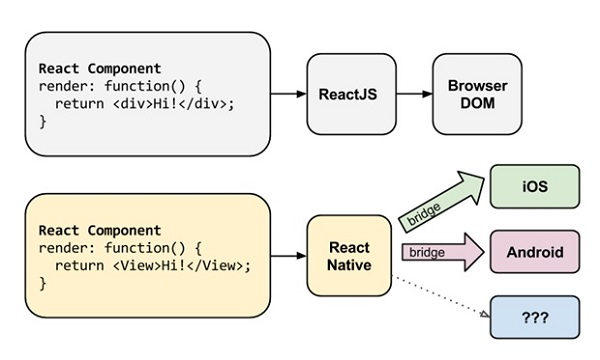
\includegraphics[scale=0.7]{obrazky/react_native}
\par\end{centering}
\caption{Diagram fungování frameworku React Native \cite{react_native_intro} \label{fig:react_native_intro}}
\end{figure}
\FloatBarrier

\addcontentsline{toc}{chapter}{Literatura} 

\begin{thebibliography}{10}

\bibitem{simon_spa} \textit{MAREŠ, Šimon}. Využití JavaScriptu pro single-page aplikaci vytvářející dokumenty. Bakalářská práce. 2015. Mendelova univerzita v Brně. Provozně ekonomická fakulta. Brno

\bibitem{mathiasson-isomorphic} \textit{MATHIASSON, Eric}. Isomorphic web applications: Depends on how you react. Sundsvall, Švédsko, 2015. Mid Sweden University. Vedoucí práce Stefan Forsstrom.

\bibitem{zakas_js} \textit{ZAKAS, Nicholas C}. JavaScript pro webové vývojáře. Brno: Computer Press, 2009, 832 s. ISBN 978-80-251-2509-0.

\bibitem{flanagan_javascript} \textit{FLANAGAN, D}. JavaScript: The Definitive Guide. 6th ed. Sebastopol, CA: O’Reilly, 2011, xvi, 1078 p. ISBN 05-968-0552-7.

\bibitem{statcounter} \textit{STATCOUNTER} StatCounter Global Stats. Top 5 Desktop, Tablet \& Console Browsers from July 2015 to July 2016. [online] [cit. 2016-08-05] Dostupné z WWW: \url{http://gs.statcounter.com/#browser-ww-monthly-201507-201607-bar}

\bibitem{hronek_javascript} \textit{HRONEK, Jakub}. Využití jazyka JavaScript v moderních aplikacích. Bakalářská práce. Mendelova univerzita v Brně. Provozně ekonomická fakulta. 2013 Brno

\bibitem{skriptovaci_jazyky} \textit{VORÁČEK, Jan}. Skriptovací jazyky pro tvorbu webových aplikací. Diplomová práce. 2013. Univerzita Pardubice. Fakulta elektrotechniky a informatiky. Pardubice

\bibitem{githut} \textit{ZAPPONI, Carlo}. Githut - a small place to discover languages in Github [online] 2016 [cit. 2016-07-17] Dostupné z WWW: \url{https://githut.info}

\bibitem{ecmascript} \textit{ECMA} ECMAScript Documentation. Ecmascript.org [online]. 2016 [cit. 2016-06-21]. Dostupné z: \url{http://www.ecmascript.org/docs.php}

\bibitem{exploring_es6} \textit{RAUSCHMAYER, Axel}. Exploring ES6. [online] [cit. 2016-07-12] Dostupné z WWW: \url{http://exploringjs.com/es6/}

\bibitem{tc39ecma} \textit{ECMA} The TC39 process for ECMAScript features. ECMAScript [online] [cit. 2016-06-21] Dostupné z WWW: \url{https://tc39.github.io/process-document/}

\bibitem{es6} \textit{ENGELSCHALL Ralf. S}. ECMAScript 6 - New features: Overview \& Comparison. [online] [cit. 2016-07-10] Dostupné z WWW: \url{http://es6-features.org/}

\bibitem{learning_es6} \textit{PRUSTY, Narayan}. Learning ECMAScript 6. Packt Publishing Ltd, 2015.

\bibitem{es6_book} \textit{SIMPSON, Kyle, et al}. You Don't Know JS: ES6 \& Beyond. " O'Reilly Media, Inc.", 2015.

\bibitem{transpilers} \textit{GUTHRIE, G}. Your transpiler to JavaScript toolbox.
[online] [cit. 2016-06-15] Dostupné z WWW: \url{http://luvv.ie/2014/01/21/your-transpilerto-javascript-toolbox}

\bibitem{babel} \textit{BABELJS}. BabelJS, compiler for writing next generation JavaScript. [online] [cit. 2016-06-15] Dostupné z WWW: \url{https://babeljs.io/}

\bibitem{coffeescript_founder} \textit{ASHKENAS, Jeremy}. Coffeescript. 2012.

\bibitem{coffeescript} \textit{COFFEESCRIPT}. CoffeeScript Documentation [online]. [cit. 2016-07-10]. Dostupné z WWW: \url{http://coffeescript.org/}

\bibitem{babel_what} \textit{VELCHEVSI, M}.  What exactly is BabelJs?: Why does it understand JSX/React components? In: Quora [online]. Mountain View, CA , U.S.: Quora, Inc., 2015 [cit. 2016-08-01]. Dostupné z WWW: \url{https://www.quora.com/What-exactly-is- BabelJs-Why-does-it-understand-JSX-React-components}

\bibitem{nodejs} \textit{NODEJS}. Node.js Documentation 2016 [cit. 2016-07-11] Dostupné z WWW: \url{https://nodejs.org/api/}

\bibitem{glover_nodejs} \textit{GLOVER, Andrew.} Node.js for Java developers. In: IBM developerWorks [online]. 2011 [cit. 2016-12-7]. Dostupné z WWW: \url{http://www.ibm.com/developerworks/java/library/j-nodejs/index.html}.

\bibitem{tilkov_nodejs} \textit{TILKOV, Stefan. VINOSKI Steve}. Node. js: Using JavaScript to build high‐performance network programs. 2010. IEEE Internet Computing. roč. 14, č. 6, s. 0080–83.

\bibitem{elektron} \textit{ELECTRON}. Electron Documentation [online] [cit. 2016-08-07] Dostupné z WWW \url{http://electron.atom.io/}

\bibitem{nodejs_numbers} \textit{NODESOURCE} Node by numbers. [Online] 2015 [cit. 2016-07-11] Dostupné z WWW: \url{https://nodesource.com/assets/blog/node-by-numbers/node-by-numbers.pdf}

\bibitem{npm} \textit{NPM.JS} Npm.js - Package manager. Installs, publishes and manages node programs. [online] [cit. 2016-07-28] Dostupné z WWW: \url{https://www.npmjs.com/}

\bibitem{task_runners} \textit{ODELL, Den}. Build Tools and Automation. In: Pro JavaScript Development. Apress, 2014. p. 391-422.

\bibitem{linter} \textit{WALSH David}. ESLint [online] [cit. 2016-06-30] Dostupné z WWW: \url{https://davidwalsh.name/eslint}

\bibitem{grunt} \textit{LI, Daniel}. Mastering Grunt. Packt Publishing Ltd, 2014. ISBN: 9781783980925

\bibitem{gulp} \textit{RENAUX, Julien}. Intruduction to Gulp.js with practical examples [online] [cit. 2016-07-20] Dostupné z WWW: \url{http://julienrenaux.fr/2014/05/25/introduction-to-gulp-js-with-practical-examples/}

\bibitem{gulp_web} \textit{GULP.JS} Gulp.js. Documentation [online] [cit. 2016-07-20] Dostupné z WWW: \url{http://gulpjs.com/}

\bibitem{jquery} \textit{JQUERY} jQuery API Documentation [online] [cit. 2016-07-25] Dostupné z WWW: \url{http://api.jquery.com/}

\bibitem{jquery_book} \textit{CHAFFER, Jonathan}. Learning JQuery 1.3: Better Interaction and Web Development with Simple JavaScript Techniques. Packt Publishing Ltd, 2009. ISBN: 9781847192509

\bibitem{jquery_ui} \textit{JQUERY} jQuery UI web components [online] [cit. 2016-07-25] Dostupné z WWW: \url{https://jqueryui.com/}

\bibitem{angular} \textit{GOOGLE Inc.} AngularJS API Docs [online]. 2014 [cit. 2016-07-20]. Dostupné z WWW: \url{https://docs.angularjs.org}

\bibitem{spa_horyna} \textit{HORYNA, Marek}. Single Page Aplikace S využitím MVVM frameworků AngularJS a React. Bakalářská práce. Univerzita Hradec Králové, Fakulta informatiky a managementu. 2015. Hradec Králové

\bibitem{react} \textit{FACEBOOK Inc.} React JS Documentation. [online] [cit. 2016-07-20] Dostupné z WWW: \url{http://facebook.github.io/react}.

\bibitem{react_book} \textit{BAGNARDI, Frankie. BEEBE, Jonathan, FELDMAN, Richard, HALLETT, Tom,  HOJBERG, Simon. MIKKELSEN, Karl.} Developing a React Edge. The JavaScript Library for User Interfaces. 2014 Bleeding Edge Press ISBN: 9781939902122

\bibitem{react_intro} \textit{GACKENHEIMER, C.}  Introduction to React. 1st ed. New York, NY, U.S.: Apress Media, 2015. ISBN: 978-1484212462.

\bibitem{spa} \textit{Single-page application} Wikipedia [Online] Dostupné z WWW: \url{https://en.wikipedia.org/wiki/Single-page_application}

\bibitem{mocha} \textit{MOCHAJS.ORG} MochaJS -  the fun, simple, flexible JavaScript test framework [online] [cit. 2016-08-08] Dostupné z WWW: \url{https://mochajs.org/}

\bibitem{zdrojak_jstesting} \textit{MROZEK, Jakub}. JavaScript na serveru: Testování a kontinuální integrace [online] 2012 [cit. 2016-08-08] Dostupné z WWW: \url{https://www.zdrojak.cz/clanky/javascript-na-serveru-testovani-a-kontinualni-integrace/}

\bibitem{jstesting} \textit{JOHANSEN, Christian}. Test-Driven JavaScript Development (Developer's Library) 1st Edition. Amazon. ISBN: 978-0321683915

\bibitem{should_js}\textit{SHOULD.JS}. Should.js API Documentation [online] [cit. 2016-08-08] Dostupné z WWW: \url{https://shouldjs.github.io/}

\bibitem{supertest}\textit{SUPERTEST}. Supertest API Documentation [online] [cit. 2016-08-08] Dostupné z WWW: \url{https://github.com/visionmedia/supertest}

\bibitem{selenium}\textit{SELENIUM}. Selenium Documentation [online] [cit. 2016-08-08] Dostupné z WWW: \url{http://www.seleniumhq.org/}

\bibitem{karma} \textit{KARMA}. Karma - Spectacular Test Runner for Javascript [online] [cit. 2016-08-08] Dostupné z WWW: \url{https://karma-runner.github.io/1.0/index.html}

\bibitem{enzyme} \textit{AIRBNB}. Enzyme Documentation [online] [cit. 2016-08-08] Dostupné z WWW: \url{http://airbnb.io/enzyme/}

\bibitem{testing_react} \textit{MENGER, David}. Testujeme React komponenty s Karmou a Enzyme. [online] 2016 [cit. 2016-08-08] Dostupné z WWW: \url{http://nodejsfan.com/testovani-karma-react-mocha/}

\bibitem{osmani_spa} \textit{OSMANI, Addy}. Developing Backbone.js Applications [online]. 2013 [cit. 2016-07-10]. Dostupné z WWW: \url{http://addyosmani.github.io/backbone-fundamentals/}

\bibitem{spa_book} \textit{SCOTT, Emmit}. SPA Design and Architecture: Understanding Single Page Web Applications. Manning Publications Co., 2015.

\bibitem{spa_web} \textit{TAKADA, Mikito}. Single page applications book. [Online] [cit. 2016-07-10] Dostupné z WWW: \url{http://singlepageappbook.com/}

\bibitem{spa_diagram} \textit{WASSON, Mike.} ASP.NET - Single-Page Applications: Build Modern, Responsive Web Apps with ASP.NET [online] [cit. 2016-07-06] 

\bibitem{crawler_spa} \textit{ SPHINX, Q}. Make Single Page Applications Crawlable [online] [cit. 2016-07-11] Dostupné z WWW: \url{http://best-web-creation.com/articles/view/id/crawlable-spa?lang=en}

\bibitem{xhr} \textit{W3C CONSORTIUM}. XMLHttpRequest Level 2, W3C Working Draft 17 January 2012. [online] [cit. 2016-07-11] Dostupné z WWW:\url{http://www.w3.org/TR/XMLHttpRequest2/}.

\bibitem{ria} \textit{KAY, Russell}. Rich Internet applications. In: Computerworld [online]. 2009-07-06 [cit. 2016-07-20]. Dostupné z WWW: \url{http://www.computerworld.com/s/article/ 335519/Rich_Internet_Applications}

\bibitem{janovsky_html5} \textit{JANOVSKÝ, Dušan}. HTML 5.  2015 Jakpsatweb.cz [online]. [cit. 2016-07-17]. Dostupné z WWW: \url{http://www.jakpsatweb.cz/html/html-5.html}

\bibitem{css3} \textit{W3C CONSORTIUM}. CSS3 Documentation [online] [cit. 2016-07-17]. Dostupné z WWW: \url{http://www.w3schools.com/css/css3_intro.asp}

\bibitem{html5_css3_book} \textit{FRAIN, Ben}. Responsive web design with HTML5 and CSS3. Packt Publishing Ltd, 2012. ISBN: 9781784398934

\bibitem{mobile_popularity} \textit{KEMP, Simon}. 2016. Digital in 2016. Wearesocial.com Dostupné z WWW: \url{http://wearesocial.com/uk/special-reports/digital-in-2016}

\bibitem{responsive_design} \textit{GARDNER, Brett S}. Responsive web design: Enriching the user experience. Sigma Journal: Inside the Digital Ecosystem, 2011, 11.1: 13-19.

\bibitem{modernizr} \textit{MODERNIZR}. Modernizr - Respond to your user’s browser features. [online] [cit. 2016-08-07] Dostupné z WWW: \url{https://modernizr.com/}

\bibitem{todomvc} \textit{TODOMVC}. TodoMVC - Helping you select an MV* framework [online] [cit. 2016-08-07] Dostupné z WWW: \url{http://todomvc.com/}

\bibitem{google_crawler} \textit{GOOGLE Inc}. Making AJAX applications crawlable [online] [cit. 2016-08-08] Dostupné z WWW: \url{https://developers.google.com/webmasters/ajax-crawling/docs/learn-more}

\bibitem{prerender} \textit{PRERENDER.IO}. Prerender.io - Allows your Javascript website to be crawled perfectly by search engines. [online] [cit. 2016-08-08] Dostupné z WWW: \url{https://www.prerender.io}

\bibitem{universal_js}\textit{JACKSON, Michael}. Universal JavaScript [cit. 2016-06-21] Dostupné z WWW: \url{https://medium.com/@mjackson/universal-javascript-4761051b7ae9}

\bibitem{isomorphic_founder} \textit{ROBBINS, Charlie}. Scaling isomorphic Javascript code [online] 2011 [cit. 2016-08-01] Dostupné z WWW: \url{https://blog.nodejitsu.com/scaling-isomorphic-javascript-code/}

\bibitem{isomorphic_airbnb2} \textit{BREHM, Spike}. Isomorphic javascript, future of web apps. [online] 2013 [cit. 2016-07-22] Dostupné z WWW: \url{http://nerds.airbnb.com/isomorphic-javascript-future-web-apps/}

\bibitem{netflix} \textit{BAXTER, Kris}. Making Netflix.com faster [online] [cit. 2016-07-22] Dostupné z WWW: \url{http://techblog.netflix.com/2015/08/making-netflixcom-faster.html}

\bibitem{isomorhic_book} \textit{STRIMPEL Jason, MAXIME Najim}. Building Isomorphic JavaScript Apps From Concept to Implementation to Real-World Solutions. 2015 O'Reilly Media

\bibitem{bower} {BOWER}. Bower - A package manager for the web - Documentation [online] [cit. 2016-07-22] Dostupné z WWW: \url{https://bower.io}

\bibitem{spa_perf} \textit{BENDER, John. PARKER, Todd, JEHL, Scott}. Research: Performance Impact of Popular JavaScript MVC Frameworks [online] [cit. 2016-07-20] Dostupné z WWW: \url{https://www.filamentgroup.com/lab/mv-initial-load-times.html}

\bibitem{isomorphic_airbnb} \textit{BREHM, Spike}. Master Class: Isomorphic Javascript [online] 2013 [cit. 2016-07-22] Dostupné z WWW: \url{http://www.slideshare.net/spikebrehm/a-28174727}

\bibitem{codepicnic_universaljs} \textit{LEON, Gustavo}. Universal JavaScript and the future of the Single Page Apps, [Online] [cit. 2016-07-10] Dostupné z WWW: \url{http://singlepageappbook.com/}

\bibitem{isomorphic_def} \textit{WOLFRAM RESEARCH}. Wolfram MathWorld - Isomorphism definition [online] [cit. 2016-08-08] Dostupné z WWW: \url{http://mathworld.wolfram.com/Isomorphism.html}

\bibitem{flux} \textit{FACEBOOK Inc.} Flux, "Application Architecture for Building User Interfaces" [online] [cit. 2016-07-27] Dostupné z WWW: \url{https://facebook.github.io/flux/docs/overview.html}

\bibitem{cordova} \textit{THE APACHE SOFTWARE FOUNDATION}. Apache Cordova Documentation [online] [cit. 2016-07-28] Dostupné z WWW: \url{https://cordova.apache.org/docs/en/latest/}

\bibitem{mobile_apps} \textit{HEITKÖTTER, Henning; HANSCHKE, Sebastian; MAJCHRZAK, Tim A}. Evaluating cross-platform development approaches for mobile applications. In: International Conference on Web Information Systems and Technologies. Springer Berlin Heidelberg, 2012. p. 120-138.

\bibitem{ionic} \textit{DRIFTY CO} Ionic framework Documentation [online] [cit. 2016-07-28] Dostupné z WWW: \url{http://ionicframework.com/}
 
\bibitem{virtualdom} \textit{FREED, Tony}. What is Virtual DOM. Tony Freed Blog [online]. [cit. 2016-07- 20]. Dostupné z WWW: \url{http://tonyfreed.com/blog/what_is_virtual_dom}

\bibitem{express} \textit{STRONGLOOP, IBM}. Express JS Documentation [online] [cit. 2016-08-08] Dostupné z WWW: \url{https://expressjs.com/}

\bibitem{immutablejs} \textit{FACEBOOK Inc.} Immutable.JS [online] [cit. 2016-08-04] Dostupné z WWW: \url{https://facebook.github.io/immutable-js/}

\bibitem{immutablejs_learn} \textit{NAGY, Zsolt}. Introduction to immutable.js [online] 2015 [cit. 2016-08-04] Dostupné z WWW: \url{http://www.zsoltnagy.eu/introduction-to-immutable-js}

\bibitem{immutability} \textit{JOHANSEN, Christian}. Immutability in JavaScript [online] [cit. 2016-08-04] Dostupné z WWW: \url{https://www.sitepoint.com/immutability-javascript/}

\bibitem{immutability_graph} \textit{PEYROTT, Sebastián}. Introduction to Immutable.js and Functional Programming Concepts. Auth0 [online] [cit. 2016-08-04] Dostupné z WWW: \url{https://auth0.com/blog/intro-to-immutable-js/}

\bibitem{immutable_json} \textit{MÁRQUEZ, Javier}. A JSON editor with React and Immutable data [online] [cit. 2016-08-04] Dostupné z WWW: \url{http://arqex.com/991/json-editor-react-immutable-data}

\bibitem{react_components} \textit{FACEBOOK Inc.} Multiple Components. In: React [online]. [cit. 2016-07-20]. Dostupné z WWW: \url{http://facebook.github.io/react/docs/multiple-components.html}.

\bibitem{react_thinking} \textit{FACEBOOK Inc.} Thinking in React. In: React [online]. [cit. 2016-07-20]. Dostupné z WWW: \url{http://facebook.github.io/react/docs/thinking-in-react.html}

\bibitem{react_inter} \textit{FACEBOOK Inc.} Interactivity and Dynamic UIs. In: React [online]. [cit. 2016-07-20]. Dostupné z WWW: \url{http://facebook.github.io/react/docs/interactivity-and-dynamic-uis.html}

\bibitem{react_why} \textit{FACEBOOK Inc.} React, "Why did we build React?" [online] [cit. 2016-07-20]
Dostupné z WWW: \url{https://facebook.github.io/react/blog/2013/06/05/why-react.html}

\bibitem{react_router} \textit{FACEBOOK Inc.} React-router [online] [cit. 2016-07-20] Dostupné z WWW: \url{https://github.com/reactjs/react-router}

\bibitem{flux_comparison} \textit{VETTER, Ricky}. We Compared 13 Top Flux Implementations. You Won’t Believe Who Came Out On Top! Med[online] [cit. 2016-07-27] Dostupné z WWW: \url{https://medium.com/social-tables-tech/we-compared-13-top-flux-implementations-you-won-t-believe-who-came-out-on-top-1063db32fe73}

\bibitem{redux} \textit{REDUX} Redux Documentation [online] [cit. 2016-08-07] Dostupné z WWW: \url{https://github.com/reactjs/redux}

\bibitem{zdrojak_gulp} \textit{OŽANA, Roman}. Gulp vs. Grunt: souboj bez vítěze a poraženého [online] 2014 [cit. 2016-07-20] Dostupné z WWW: \url{https://www.zdrojak.cz/clanky/gulp-vs-grunt-souboj-bez-viteze-a-porazeneho}

\bibitem{grunt_intro} \textit{ALMAN, Ben}. Introducing Grunt [online] 2012 [cit. 2016-07-20] Dostupné z WWW: \url{http://benalman.com/news/2012/03/introducing-grunt}

\bibitem{webpack} \textit{KOPPERS, Tobias}. Webpack Documentation. [online] [cit. 2016-08-08] Dostupné z WWW: \url{https://github.com/webpack/webpack}

\bibitem{webpack_book} \textit{VEPSALAINEN, Juho. KOPPERS, Tobias. RODRÍGUEZ Rodríguez Jesús}. SurviveJS - Webpack. From apprentice to master. 2016 Leanpub

\bibitem{json} \textit{JSON}. [Online] Dostupné z WWW: \url{http://www.json.org/}.

\bibitem{ja} \textit{JOSEF, Jakub}. NoSQL databáze. Bakalářská práce. 2014 Univerzita Hradec Králové. Fakulta informatiky a managementu. Hradec Králové

\bibitem{rethinkdb} \textit{RETHINKDB} RethinkDB Documentation [online] [cit. 2016-08-09] Dostupné z WWW: \url{http://rethinkdb.com/docs/}

\bibitem{este}\textit{STEIGERWALD, Daniel}. steida/este. In: GitHub [online]. [cit. 2016-04-14]. Dostupné z WWW: \url{https://github.com/steida/este}

\bibitem{isomorphic_pimentel} \textit{PIMENTEL, Rodrigo}. How To Build Amazing Apps Using Isomorphic Applications [online] 2015 [cit. 2016-07-22] Dostupné z WWW: \url{http://blog.belatrixsf.com/how-to-build-amazing-apps-using-isomorphic-applications/}

\bibitem{ima}\textit{SEZNAM.CZ} IMA.js Documentation. [online] [cit. 2016-08-08] Dostupné z WWW: \url{https://imajs.io/}

\bibitem{meteor} \textit{HLAVÁČEK, Josef Bc.} Vývoj aplikací na platformě Meteor. Diplomová práce. 2014. Vysoká škola ekonomická v Praze. Fakulta	informatiky a statistiky. Katedra informačních	technologií. Praha

\bibitem{meteor_web} \textit{METEOR DEVELOPMENT GROUP Inc.} Meteor documentation. [online] [cit. 2016-08-08] Dostupné z WWW: \url{https://docs.meteor.com}

\bibitem{derbyjs} \textit{DERBYJS} DerbyJS Documentation. [online] [cit. 2016-08-08] Dostupné z WWW: \url{http://derbyjs.com/docs/}

\bibitem{rendrjs} \textit{RENDRJS} RendrJS Documentation. [online] [cit. 2016-08-08] Dostupné z WWW: \url{http://rendrjs.github.io/}

\bibitem{react_best_practices}\textit{EARLY, Alex}. REACT TIPS AND BEST PRACTICES. aeflash.com [online] [cit. 2016-08-10] Dostupné z WWW: \url{http://aeflash.com/2015-02/react-tips-and-best-practices.html}

\bibitem{stylus} \textit{STYLUS} Stylus Documentation. [online] [cit. 2016-08-11]. Dostupné z WWW: \url{http://stylus-lang.com/}

\bibitem{websocket} \textit{MOZILLA DEVELOPER NETWORK} WebSockets. Mozilla Developer Network [online] [cit. 2016-08-11] Dostupné z WWW: \url{https://developer.mozilla.org/en-US/docs/Web/API/WebSockets_API}

\bibitem{socketio} \textit{SOCKET.IO} Socket.io Documentation [online] [cit. 2016-08-11] Dostupné z WWW: \url{http://socket.io/docs/}

\bibitem{knesl} \textit{KNESL, Jiří.} Isomorfní aplikace nejsou budoucnost [online] [cit. 2016-08-14] Dostupné z WWW: \url{http://www.knesl.com/izomorfni-aplikace-nejsou-budoucnost}

\bibitem{react_css}\textit{FACEBOOK Inc.} React tips: Inline styles [online] [cit. 2016-08-18]  Dostupné z WWW: \url{https://facebook.github.io/react/tips/inline-styles.html}

\bibitem{inline_styles_hate} \textit{COYIER, Chris}. The debate around: "Do we neww CSS anymore?" [online] CSS-Tricks [cit. 2016-08-18] Dostupné z WWW: \url{https://css-tricks.com/the-debate-around-do-we-even-need-css-anymore/}

\bibitem{react_native} \textit{FACEBOOK Inc.} React Native Documentation [online] [cit. 2016-08-18] Dostupné z WWW: \url{https://facebook.github.io/react-native/}

\bibitem{react_native_intro} \textit{EISENMAN, Bonnie}. Writing Cross-Platform Apps with React Native [online] [cit. 2016-08-18] Dostupné z WWW: \url{https://www.infoq.com/articles/react-native-introduction}

\end{thebibliography}

\cleardoublepage{}

\appendix
\pagenumbering{Roman}\addcontentsline{toc}{part}{Přílohy}\thispagestyle{empty}  \renewcommand{\appendixname}{P\v{r}iloha}%%přílohy, číslování římskými


\part*{Přílohy}


\chapter[\noindent Manuál k ukázkové webové aplikaci]{\noindent Manuál k ukázkové webové aplikaci}

Ukázková webová aplikace běží v operačních systémech Windows, Mac OS X a Linux. Jedinou závislostí je node.js. Jelikož jsou použity nové vlastnosti moderního Javascriptu, je vyžadována minimálně verze 6.0.0. Jako databáze je použita RethinkDB, které je zdarma dostupná na webu projektu. Veškeré příkazy se volají prostřednictvím příkazového řádku.

\section*{Požadavky na systém}
\begin{itemize}
\item Node.js - minimálně verze 6
\item NPM - minimálně verze 3.10
\item RethinkDB - minimálně verze  2.3
\end{itemize}


\section*{Instalace a spuštění aplikace} 

\noindent\textbf{1. Nainstalování veškerých závislostí}

\begin{lstlisting}[language=Javascript]
npm intall
\end{lstlisting}

\noindent\textbf{2. Naplnění databáze testovacími daty}
\begin{lstlisting}[language=Javascript]
npm run db-setup
\end{lstlisting}

\noindent\textbf{3. Spuštění vývojového serveru}

\vspace{3mm}
Linux / Mac OS X:
\begin{lstlisting}[language=Javascript]
npm start
\end{lstlisting}

Windows:
\begin{lstlisting}[language=Javascript]
npm run start:win
\end{lstlisting}

Pokud vše proběhlo bez chyb, je ukázková isomorfní webová aplikace dostupná na adrese \textit{http://localhost:3001}.

\section*{Dostupné tasky v NPM}
Tasky se spouští pomocí příkazu \textit{npm run NAZEV\_TASKU}.

\begin{itemize}
\item \textbf{build:prod} – vytvoří balíček aplikace pro nasazení na server,
\item \textbf{db-setup} – připraví databázi pro vývoj,
\item \textbf{lint} – lintování kódu,
\item \textbf{start} – spuštění aplikace ve vývojovém módu,
\item \textbf{start:win} – spuštění aplikace ve vývojovém módu na platformě Windows,
\item \textbf{start:prod} – spuštění aplikace v produkčním módu,
\item \textbf{test} – spuštění testů.
\end{itemize}



\appendix
\pagenumbering{Roman}


\chapter*{Seznam zkratek}
\begin{itemize}
\item AJAX - Asynchronous JavaScript and XML
\item API - Application Programming Interface
\item CPU Central Processing Unit
\item CSS - Cascading Style Sheet
\item DOM - Document Object Model
\item GPU - Graphical Processing Unit
\item HTML - Hypertext Markup Language HTML5 HTML version 5
\item HTTP - Hypertext Transfer Protocol
\item JSON - JavaScript Object Notaion
\item MVC - Model-View-Controller
\item OOP -  Object-oriented Programming
\item PNG - Portable Network Graphics
\item RIA - Rich Internet Application
\item REST - Representational State Transfer
\item SPA - Single Page Application
\item SVG - Scalable Vector Graphics
\item UI - User Interface
\item URL - Uniform Resource Location
\item VDOM Virtual Document Objekt Model
\item XML - Extensible Markup Language
\end{itemize}
\listoffigures
\listoftables
\lstlistoflistings

%zadani
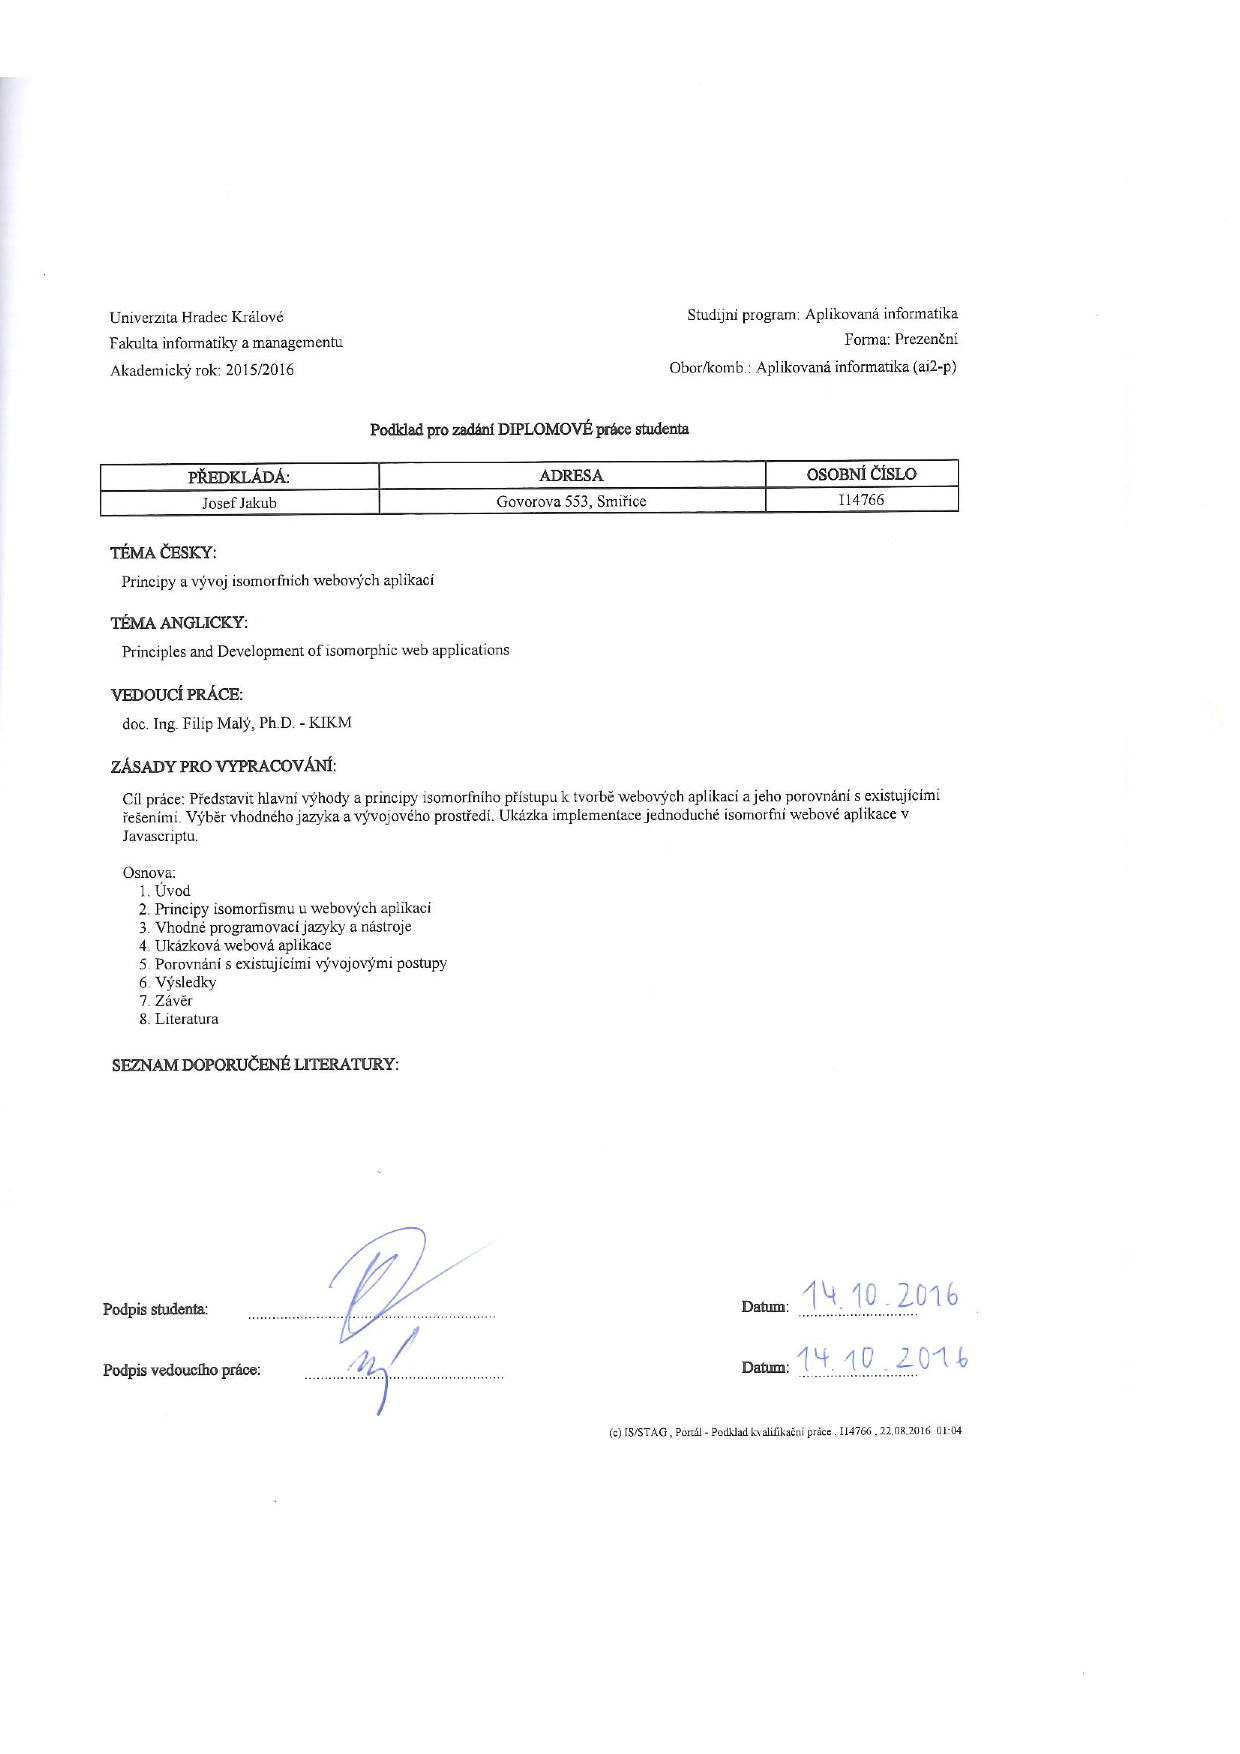
\includepdf[pages={1},scale=0.8]{zadani2}

\clearpage{}
\end{document}